%% ----------------------------------------------------------------
%% tesis.tex -- MAIN FILE (the one that you compile with LaTeX)
%% ----------------------------------------------------------------

\documentclass[a4paper, 12pt, oneside]{JMtesis}

% Location of the graphics files (set up for graphics to be in PDF format)
%\graphicspath{images/}
\graphicspath{/home/jm95/Documents/TESIS/tesis_latex/JM_tesis/images}

% Include any extra LaTeX packages required
\usepackage[square, numbers, comma, sort&compress]{natbib}
\usepackage{verbatim}  %
\usepackage{caption}
\usepackage{amsmath}
\usepackage{esvect}
%\usepackage{subfig}
%\usepackage{subcaption}

\hypersetup{urlcolor=blue, colorlinks=true}
\usepackage{multirow}
\newcommand{\grad}{$^{\circ}$}
% For Spanish
\usepackage[utf8]{inputenc}
\newcommand{\x}{\mathbf x}
\newcommand{\X}{\mathnormal x}
\newcommand{\y}{\mathnormal y}
\newcommand{\z}{\mathnormal z}
\newcommand{\q}{\mathbf q}
\newcommand{\mayusx}{\mathnormal X}
\newcommand{\mayusy}{\mathnormal Y}
\newcommand{\mayusz}{\mathnormal Z}

%% ============================================================================
\begin{document}

\frontmatter
\department{Ingeniería Electrónica}
\degree{Ingeniero Electrónico}
%\title {DESARROLLO DE UN ALGORITMO AUT\'ONOMO, PARA LA NAVEGACI\'ON DE UN ROBOT M\'OVIL, APLICADO A LA INSPECCI\'ON DE SOCAVONES SUBTERR\'ANEOS}
\title {DESARROLLO DE UN SISTEMA DE EXPLORACIÓN Y MAPEO EN TRES DIMENSIONES PARA UN ROBOT MÓVIL}
\author{Jos\'e Mar\'ia Muñoz Huam\'an}
\authorid{201210145}
%\supervisor{Oscar E. Ramos Ponce}
\supervisor{Oscar E. Ramos}
\date{Noviembre 2018}

\maketitle
\setstretch{1.5}

%\input{headers/aprobacion}
%%% ============================================================================
%  Dedicatoria
%% ============================================================================

\dedicatory{
A mi madre Flor de Luz.\\
Por haberme apoyado en todo momento, por sus consejos, sus valores, por la 
motivación constante que me ha permitido ser una persona de bien, pero más 
que nada, por su amor.
}

%%% ============================================================================
%  Página de Agradecimientos
%% ============================================================================

\acknowledgements{

A Oscar Ramos, por su amistad, paciencia y confianza depositada en mí.

A Victor Murray, por su amistad y paciencia, además por haber tomado su 
tiempo en leer este trabajo de tesis.

A mis amigos que me brindaron siempre su apoyo y por todos sus 
consejos. Juan Llanos, Luis Sanchez, Luis Montaño y Franco Lama.

}



\tableofcontents
%\listoftables
\listoffigures
\resumen

Esto es un ejemplo de resumen para próximo escrito.Esto es un ejemplo de resumen para próximo 
escrito.Esto es un ejemplo de resumen para próximo escrito.Esto es un ejemplo de resumen para próximo 
escrito.Esto es un ejemplo de resumen para próximo escrito.Esto es un ejemplo de resumen para próximo 
escrito.Esto es un ejemplo de resumen para próximo escrito.Esto es un ejemplo de resumen para próximo 
escrito.Esto es un ejemplo de resumen para próximo escrito.Esto es un ejemplo de resumen para próximo 
escrito.Esto es un ejemplo de resumen para próximo escrito.Esto es un ejemplo de resumen para próximo 
escrito.Esto es un ejemplo de resumen para próximo escrito.Esto es un ejemplo de resumen para próximo 
escrito.Esto es un ejemplo de resumen para próximo escrito.Esto es un ejemplo de resumen para próximo 
escrito.Esto es un ejemplo de resumen para próximo escrito.Esto es un ejemplo de resumen para próximo 
escrito.Esto es un ejemplo de resumen para próximo escrito.Esto es un ejemplo de resumen para próximo 
escrito.Esto es un ejemplo de resumen para próximo escrito.Esto es un ejemplo de resumen para próximo 
escrito.Esto es un ejemplo de resumen para próximo escrito.Esto es un ejemplo de resumen para próximo 
escrito.Esto es un ejemplo de resumen para próximo escrito.Esto es un ejemplo de resumen para próximo 
escrito.Esto es un ejemplo de resumen para próximo escrito.Esto es un ejemplo de resumen para próximo 
escrito.Esto es un ejemplo de resumen para próximo escrito.Esto es un ejemplo de resumen para próximo 
escrito.Esto es un ejemplo de resumen para próximo escrito.Esto es un ejemplo de resumen para próximo 
escrito.Esto es un ejemplo de resumen para próximo escrito.
\addtocontents{toc}{\vspace{1.5em}}

%% ============================================================================
\mainmatter
\pagestyle{fancy}

%\intro{
Actualmente, diversos métodos de explotación son utilizados en la minería 
subterránea para la extracción de minerales. Los más utilizados en el Perú 
son variaciones del método de corte y relleno ascendente como descendente. La 
presente tesis se enfoca en el método de corte y relleno ascendente, ya que es el 
más utilizado en el Perú \cite{Cruz2012}. 

En el método de corte y relleno ascendente el mineral es arrancado por franjas 
horizontales y/o verticales empezando por la parte inferior de un tajo y avanzando 
verticalmente. Cuando se ha extraído la franja completa, se rellena el volumen 
correspondiente con material estéril (relleno), que sirve de piso de trabajo a 
los obreros y al mismo tiempo permite sostener las paredes y el 
techo \cite{MunozDelPino2012}. Asimismo, se utiliza grandes máquinas que construyen 
socavones subterráneos por donde se va a extraer los minerales. 

La construcción de socavones subterráneos es de gran importancia para la minería 
subterránea, debido a que por medio de esta construcción se extrae los minerales 
de la mena (roca mineralizada). Estas construcciones son de diversos tamaños  en 
las diferentes unidades mineras del Perú, que dependen del tamaño de las máquinas
que van a ingresar para la extracción del mineral. Durante el proceso de construcción
pueden ocurrir diferentes riesgos (desprendimiento de rocas, emisión de gases, etc.) 
que ponen en peligro la vida de los trabajadores. Para evitar los riesgos dentro de 
la minería subterránea, se necesita supervisar la zona de construcción y a la par 
obtener una representación geométrica visual de toda la excavación. En la minería 
subterránea, para la supervisión y la generación del mapa topográfico los 
especialistas encargados son el topógrafo y el geomecánico. Se dará énfasis a 
la función del topógrafo. 

La función del topógrafo es observar la estructura de los socavones, luego medir 
las dimensiones del área y con los datos obtenidos generar el mapa topográfico. Los 
socavones subterráneos son ambientes demasiados oscuros, esto hace que existan 
limitaciones en la visión humana, por ende los topógrafos realizan un mapa del 
ambiente bastante impreciso. Estos especialistas actualmente utilizan teodolitos 
para medir el área del socavón, pero estas herramientas de medición son 
controladas manualmente, por ende las mediciones no son exactas. El tiempo 
que le toma a cada topógrafo en realizar todo su trabajo es aproximadamente entre 
3 a 4 horas, y posterior a esto el tiempo que se demora para la generación del mapa 
topográfico es entre dos a tres días. Debido a la ineficiencia en el proceso de la 
generación del mapa topográfico, hace que se retrase la producción de extracción 
de minerales dentro de la mina subterránea, ya que los ingenieros mineros 
necesitan calcular el volumen de extracción de la beta mineralizada. Las mineras 
pagan por volumen extraído.
}

\section{Justificación}

Debido al problema descrito anteriormente, la propuesta de este trabajo de tesis 
se centra en desarrollar un algoritmo de autonomía para la navegaci\'on de un robot 
m\'ovil dentro del socav\'on subterr\'aneo. Donde se elige un sensor l\'aser el 
cual es añadido al robot para su desplazamiento de manera aut\'onoma y a su vez 
construya el mapa tridimensional del socavón subterr\'aneo.

El robot m\'ovil utilizar\'a t\'ecnicas de SLAM (\textit{Simultaneous Localization 
and Mapping}) para realizar un mapa del interior del socav\'on y a su vez poder 
estimar la posici\'on de este dentro de dicho ambiente. Con respecto al sistema 
de navegaci\'on se implementar\'a un algoritmo basado en campos potenciales el 
cual va a permitir que el robot pueda generar su propia trayectoria, evitando 
colisionar con las paredes o los obst\'aculos del camino por donde se va a 
desplazar. Se tomar\'a la informaci\'on del sensor LIDAR (\textit{Light 
Detection and Ranging}) para generar el mapa topogr\'afico en dos dimensiones.

Se elige el sensor LIDAR, ya que emite impulsos r\'apidos de luz l\'aser, hasta 
4000 impulsos por segundo, sobre una superficie. Este instrumento mide la 
cantidad de tiempo necesario para que cada pulso pueda recuperarse, y a partir 
de esto calcula la distancia entre el objeto y el instrumento con una alta 
precisi\'on. Como utiliza luz l\'aser, el sensor no necesita de iluminaci\'on 
externa para realizar las mediciones, lo cual es perfecto para los socavones 
de miner\'ia subterránea ya que en estas zonas no hay una buena iluminaci\'on. 

Para realizar el mapa en tres dimensiones, se diseñar\'a un sistema mec\'anico 
que permitir\'a que el sensor l\'aser pueda tomar mediciones en diferentes 
alturas, obteniendo los datos en las tres coordenadas del sistema de 
referencia. Posteriormente, estos datos serán procesados utilizando un 
algoritmo de ICP (\textit{Iterative Closest Point}) para as\'i obtener una 
nube de puntos. Finalmente, se utilizar\'a un software para poder visualizar 
el mapa tridimensional del socavón subterr\'aneo.

\section{Alcances y limitaciones}

Para realizar el mapa topogr\'afico se debe considerar que el t\'unel subterr\'aneo 
tiene un terreno bastante accidentado y el robot m\'ovil donde fue implementado el 
algoritmo no tiene el diseño mec\'anico correspondiente para este tipo de ambiente. Por 
tal motivo el presente trabajo ser\'a capaz de moverse por un t\'unel con una superficie 
bastante recta sin cambios bruscos en la pendiente. Otra dificultad a considerar es la 
dimensi\'on de los socavones que var\'ian seg\'un el tama\~no de la beta mineralizada, por 
ende el trabajo de tesis ser\'a capaz de mapear el t\'unel que no exceda los 16 metros de 
ancho debido al rango de alcance que tiene el sensor lidar. 

Finalmente, el algoritmo de autonom\'ia puede usarse para cualquier robot m\'ovil (terrestre 
o a\'ereo) considerando que el modelo din\'amico y cinem\'atico de estos ya se encuentran 
previamente implementados. Para el caso del robot m\'ovil a\'ereo se debe tener en cuenta 
que no debe haber variaciones bruscas en la altura, se debe mantener un vuelo estable.

\section{Organizaci\'on de la tesis}

El documento está organizado en 4 capítulos los cuales serán explicados en esta
sección. En el capítulo 1 se explicará los algoritmos que se usan actualmente para el 
control de movimiento del robot móvil, la generación de trayectoria, la localización y 
mapeo de forma simultánea. En el capítulo 2 se describirá el control de movimiento que 
fue implementado, así también el algoritmo de generación de trayectoria que se utilizo, 
el algoritmo de localización y mapeo. Se explicará el diseño mecánico construido
para hacer el mapa en tres dimensiones. En el capítulo 3 se describirá y explicará con detalle
los resultados obtenidos, ya que se realizó pruebas en simulación y en un ambiente real que 
se asemeja a la estructura de un socavón subterráneo. En el capítulo 4 se expondrán las conclusiones.

%\resumen{

Hola esto es un resumen.Hola esto es un resumen.Hola esto es un resumen.Hola esto es un resumen.Hola esto es un resumen.Hola esto es un resumen.Hola esto es un resumen.Hola esto es un resumen.Hola esto es un resumen.Hola esto es un resumen.Hola esto es un resumen.Hola esto es un resumen.Hola esto es un resumen.Hola esto es un resumen.Hola esto es un resumen.Hola esto es un resumen.Hola esto es un resumen.Hola esto es un resumen.Hola esto es un resumen.Hola esto es un resumen.Hola esto es un resumen.Hola esto es un resumen.Hola esto es un resumen.Hola esto es un resumen.Hola esto es un resumen.Hola esto es un resumen.Hola esto es un resumen.Hola esto es un resumen.Hola esto es un resumen.Hola esto es un resumen.Hola esto es un resumen.Hola esto es un resumen.Hola esto es un resumen.Hola esto es un resumen.Hola esto es un resumen.Hola esto es un resumen.Hola esto es un resumen.Hola esto es un resumen.Hola esto es un resumen.Hola esto es un resumen.Hola esto es un resumen.Hola esto es un resumen.Hola esto es un resumen.Hola esto es un resumen.Hola esto es un resumen.Hola esto es un resumen.Hola esto es un resumen.Hola esto es un resumen.Hola esto es un resumen.Hola esto es un resumen.Hola esto es un resumen.Hola esto es un resumen.Hola esto es un resumen.Hola esto es un resumen.Hola esto es un resumen.Hola esto es un resumen.Hola esto es un resumen.Hola esto es un resumen.Hola esto es un resumen.Hola esto es un resumen.Hola esto es un resumen.Hola esto es un resumen.Hola esto es un resumen.Hola esto es un resumen.Hola esto es un resumen.Hola esto es un resumen.
Hola esto es un resumen.Hola esto es un resumen.Hola esto es un resumen.Hola esto es un resumen.Hola esto es un resumen.
Hola esto es un resumen.Hola esto es un resumen.Hola esto es un resumen.Hola esto es un resumen.Hola esto es un resumen.
Hola esto es un resumen.Hola esto es un resumen.Hola esto es un resumen.Hola esto es un resumen.Hola esto es un resumen.}
\chapter{INTRODUCCIÓN}

\section{Problemática}

Actualmente, diversos métodos de explotación son utilizados en minería para la extracción de minerales. Los más utilizados en minería subterránea en el Perú son variaciones del método de Corte y Relleno Ascendente como Descendente \cite{Cruz2012}. La presente tesis se enfoca en el método de Corte y Relleno Ascendente, ya que es el más utilizado en el Perú. 

En el método de Corte y Relleno Ascendente el mineral es arrancado por franjas horizontales y/o verticales empezando por la parte inferior de un tajo y avanzando verticalmente. Cuando se ha extraído la franja completa, se rellena el volumen correspondiente con material estéril (relleno), que sirve de piso de trabajo a los obreros y al mismo tiempo permite sostener las paredes y el techo \cite{MunozDelPino2012}. Asimismo, se utiliza grandes máquinas que construyen socavones subterráneos por donde se va a extraer los minerales. 

La construcción de socavones subterráneos es de gran importancia para la minería subterránea, debido a que por medio de esta construcción se extrae los minerales de la mena (roca mineralizada). Estas construcciones son de diversos tamaños  en las diferentes unidades mineras del Perú, que dependen del tamaño de las máquinas que van a ingresar para la extracción del mineral. Durante el proceso de construcción pueden ocurrir diferentes riesgos (desprendimiento de rocas, emisión de gases, etc.) que ponen en peligro la vida de los trabajadores. Para evitar los riesgos dentro de la minería subterránea, se necesita supervisar la zona de construcción y a la par obtener una representación geométrica visual de toda la excavación. En la minería subterránea, para la supervisión y la generación del mapa topográfico los especialistas encargados son el topógrafo y el geomecánico. Se dará énfasis a la función del topógrafo. 

La función del topógrafo es observar la estructura de los socavones, luego medir las dimensiones del área y con los datos obtenidos generar el mapa topográfico. Los socavones subterráneos son ambientes demasiados oscuros, esto hace que existan  limitaciones en la visión humana, por ende los topógrafos realizan un mapa del ambiente bastante impreciso. Estos especialistas actualmente utilizan teodolitos para medir el área del socavón, pero estas herramientas de medición son controladas manualmente, por ende las mediciones no son exactas. El tiempo que le toma a cada topógrafo en realizar todo su trabajo es aproximadamente entre 3 a 4 horas, y posterior a esto el tiempo que se demora para la generación del mapa topográfico es entre dos a tres días. Debido a la ineficiencia en el proceso de la generación del mapa topográfico, hace que se retrase la producción de extracción de minerales dentro de la mina subterráneo, ya que los ingenieros mineros necesitan calcular el volumen de extracción de la beta mineralizada.



\section{Justificación}


%La propuesta de este trabajo de tesis se centra en desarrollar un robot aéreo autónomo \cite{Lopez2016} para inspeccionar los socavones subterráneos en la mina. Donde se elige un sensor láser para añadirlo al robot aéreo y así poder realizar el vuelo autónomo y el mapa tridimensional del socavón subterráneo.

%Para la inspección de socavones se elige un robot aéreo debido a que brinda muchas ventajas como:
%\begin{itemize}
%\item[•]\textit{Reducción de costos}: Un robot aéreo no necesita de carriles especiales o caminos previamente adaptados para poder ingresar al área que se desea generar el mapa topográfico.
%\item[•]\textit{Reducción de tiempos}: No se necesita ir a una pista de aterrizaje para poner en funcionamiento al robot aéreo, ya que puede funcionar en cualquier parte.
%\item[•]\textit{Zonas de difícil acceso}: Debido a sus dimensiones, maniobrabilidad y a su naturaleza, un robot aéreo puede adentrarse con facilidad en zonas accidentadas, como por ejemplo: grutas, túneles o chimeneas.
%\item[•]\textit{Adaptabilidad de aplicaciones}: Un robot aéreo tiene la posibilidad de adaptarse a diferentes aplicaciones como servicios de vigilancia, mapeos de terreno a tajo abierto, control de incendios, control de infraestructuras eólicas, etc. 
%\item[•]\textit{Reducción de riesgos laborales}: Un robot aéreo autónomo no necesita ser tripulado, por lo tanto puede adentrarse en zonas peligrosas o potencialmente peligrosas evitando el acceso riesgoso de personas. 
%\end{itemize}

%Este robot aéreo utilizará técnicas de SLAM (\textit{Simultaneous Localization And Mapping}) para realizar un mapa del interior del socavón y generar su propia trayectoria dentro del socavón, evitando colisionar con las paredes o los obstáculos del camino de manera autónoma. Se tomará la información del sensor LIDAR (\textit{Light Detection and Ranging}) para generar el mapa topográfico.

%Se elige el sensor LIDAR, ya que emite impulsos rápidos de luz láser, hasta 150.000 impulsos por segundo, sobre una superficie. Este instrumento mide la cantidad de tiempo necesario para que cada pulso pueda recuperarse, y a partir de esto calcula la distancia entre el objeto y el instrumento con una alta precisión. Como utiliza luz láser, el sensor no necesita de iluminación externa para realizar las mediciones, lo cual es perfecto para los socavones de minería subterránea ya que en estas zonas no hay una buena iluminación.

La propuesta de este trabajo de tesis se centra en desarrollar un algoritmo de autonomía para la navegación de un robot móvil, para que este se pueda desplazar de forma autónoma dentro del socavón subterráneo. Donde se elige un sensor láser el cual se añade al robot móvil para la navegación y a su vez el mapa tridimensional del socavón subterráneo.

El robot móvil utilizará técnicas de SLAM (\textit{Simultaneous Localization and Mapping}) para realizar un mapa del interior del socavón y también para poder estimar la posición de este dentro de dicho ambiente. Con respecto al sistema de navegación se implementará un algoritmo basado en Campos Potenciales para que el robot pueda generar su propia trayectoria dentro del socavón, evitando colisionar con las paredes o los obstáculos del camino por donde va de manera autónoma. Se tomará la información del sensor LIDAR (\textit{Light Detection and Ranging}) para generar el mapa topográfico en dos dimensiones (2D).

Se elige el sensor LIDAR, ya que emite impulsos rápidos de luz láser, hasta 4000 impulsos por segundo, sobre una superficie. Este instrumento mide la cantidad de tiempo necesario para que cada pulso pueda recuperarse, y a partir de esto calcula la distancia entre el objeto y el instrumento con una alta precisión. Como utiliza luz láser, el sensor no necesita de iluminación externa para realizar las mediciones, lo cual es perfecto para los socavones de minería subterránea ya que en estas zonas no hay una buena iluminación. 

Para realizar el mapa en tres dimensiones (3D), se diseñará un sistema mecánico el cual permitirá mover el sensor láser en el eje $Z$, obteniendo los datos en las tres coordenadas del sistema de referencia del láser. Posteriormente, estos datos serán procesados utilizando un algoritmo de ICP (\textit{Iterative Closest Point}) para así obtener una nube de puntos. Luego de este proceso, se utilizará un software para poder visualizar los datos y así obtener el mapa tridimensional del socavón subterráneo.
 
\section{Objetivos}

\subsection{General}
Desarrollar un algoritmo para la navegación autónoma de un robot móvil para inspeccionar los socavones subterráneos en la mina basado en un sistema de sensado láser. 
\\
\subsection{Específicos}
\begin{itemize}
\item[•]Diseñar e implementar el algoritmo de campos potenciales para un robot móvil.
\item[•]Diseñar e implementar un controlador para la posición y orientación del robot móvil.
\item[•]Implementar el método SLAM con el sensor LIDAR.
\item[•]Configurar la interface del usuario en el sistema operativo ROS (\textit{Robot Operating System}) para la visualización del entorno donde se desplaza el robot móvil.
\end{itemize}


\chapter{ESTADO DEL ARTE}

\section{Robótica en Minería}
La minería actual ha llevado a que las compañías mineras busquen la eficiencia incorporando la robótica a sus procesos, generando, adicionalmente, una fuente fructífera de innovación local. Actualmente el país sudamericano con mayor inversión en minería es el país de Chile, este país ha iniciado la robótica en su país hace unos 15 años. “Por el año 2000 comenzaron los primeros esfuerzos en introducir mecanismos robóticos en la minería”, señalo Carlos Carmona, gerente general de MIRS (\textit{Mining Industry Robotic Solutions})\cite{Carmona2014}.

Los beneficios potenciales de los robots en la minería subterránea son abundantes. Debido a que estas zonas son entornos de trabajo extenuante y potencialmente peligroso para los seres humanos. Por tal motivo, dándole un mayor grado de autonomía a los robots, estos se convierten en buenos ayudantes para los mineros o incluso pueden sustituir el personal que se despliega en los socavones \cite{Carmona2014}. Hace 20 años se empezó a realizar investigaciones sobre autonomía en la minería subterránea utilizando una máquina de carga con sensores láser y de ultrasonido que transportaba los minerales por las minas subterráneas (1999) \cite{Scheding1999}. 

Este trabajo  de investigación  se enfoca en la inspección de socavones subterráneos, por ende en el año 2003 “\textit{Groundhog}” fue el primer robot que exploró la mina de Florencia (\textit{New Eagle}) \cite{Thrun2004}, empleando sensores láser y una cámara de video. Asimismo en Alemania se creó un robot móvil llamado “\textit{Alexander}” el cual exploró la mina de oro \textit{Reiche Zeche} en Freiberg (2014) \cite{Grehl2015}.

Para la generación de los modelos geométricos visuales en 3D como primer trabajo en el año 2014 se utilizó una camioneta equipada de sensores láser y un microprocesador, los cuales ayudaron a realización de un modelo en 3D de la mina \cite{Zlot2014}. Como trabajo a futuro de esta investigación, es pasar el software, para obtener el modelo visual 3D, a un robot móvil.
 
El robot utilizará la técnica SLAM para su desplazamiento. Anteriores trabajos respaldan en que este método es la más adecuada para la autonomía del robot, así como es en el caso del robot móvil minero “\textit{QHUBOT}” , que utiliza la técnica FastSLAM para poder desplazarse sobre los socavones subterráneos \cite{Mauricio2015}, así también en \cite{Thrun2004} utilizan la técnica de SLAM para la exploración de la mina abandona. 

Actualmente, hay trabajos de investigación en los que estudian drones con el algoritmo SLAM  donde unos se orientan a resolver problemas de navegación utilizando algoritmos de seguimiento de líneas basados en la visión \cite{Verschoor2013}. El algoritmo basado en la visión se emplea en las diversas estructuras lineales, que reflejan el entorno construido por los seres humanos, donde se implementa un algoritmo SLAM acompañado de los puntos que detecta una cámara. Así la misma lógica del uso de SLAM se refleja en el paper \cite{Skoda2015} solo que los autores describen el uso de drones en la situación muy especializado como lo son de rescate. El objetivo es enviar el drone para que genere un mapa 3D antes de enviar al personal de emergencias. El mapa es generado por la costura de varias imágenes de una cámara RGBD (\textit{RGB y profundidad de imagen}). Algo similar se puede ver en el paper \cite{Heukels2015} el cual el algoritmo SLAM se utiliza después de realizar procesamiento de imágenes a las imágenes obtenidas de una cámara.

Comercialmente existe drones que cumplen la función buscada (\textit{generar mapas}), como es el caso de la empresa Canadiense llamada \textit{Clickmox Solutions}, que ha desarrollado un drone llamado “\textit{MineFly Drone}”, el cual tiene un escáner láser que genera mapas en las minas subterráneas. El drone está integrado con una luz LED, sensores sonar, una cámara HD y emplea la técnica de SLAM para poder desplazarse por todo el socavón sin la necesidad de utilizar un GPS \cite{Solutions2016}. 

\section{Navegación del Robot Móvil}

Un robot es un sistema autónomo que puede percibir su entorno y actuar para poder alcanzar sus objetivos. Un robot móvil dentro de un entorno no se encuentra en una ubicación específica, ya que este tiene la capacidad de moverse en su entorno. La principal característica que define a un robot autónomo es la capacidad de actuar sobre la base de sus propias decisiones, y no a través del control de un ser humano \cite{mataric2007robotics}.

La navegación se define como el proceso o la actividad de determinar con exactitud la posición de uno mismo, planificar y seguir una ruta. En robótica, la navegación se refiere a la forma en que un robot encuentra su camino en el entorno, es una necesidad y requisito común para casi todos los robots móviles.

La navegación de robots es un campo bastante extenso y se puede dividir en subcategorías para una mejor comprensión de los problemas. Leonard and Durrant-Whyte \cite{leonard1991mobile}, describen brevemente el problema general de la navegación de los robots móviles en tres simples preguntas, cada una refiriendose a una subcategoría:
\begin{itemize}
\item[•] \textbf{``¿Dónde estoy?"}\\
Esta pregunta constituye el problema de localización que se puede expresar como: Un robot se encuentra en una posición desconocida en un entorno para el que tiene un mapa. ``Observa" su posición y, basándose en estas observaciones, debe inferir el lugar o conjunto de lugares en el mapa donde podría ubicarse.
\item[•] \textbf{``¿A dónde voy?"}\\
El problema de mapeo consiste en que un robot se encuentra en un entorno desconocido para el cual no tiene un mapa, y al navegar a través de él se habilita la creación de una representación de mapa. El robot debe identificar las características especiales en los puntos de referencia del entorno para reconocer dónde se encuentran los obstáculos.
\item[•] \textbf{``¿Cómo llego hasta ahí?"}\\
El problema de la planificación de la ruta es una preocupación general por encontrar rutas que conecten diferentes ubicaciones en un entorno con objetivos específicos y limitaciones.
\end{itemize}

La navegación actualmente es un problema difícil y complejo, con muchas soluciones y enfoques diferentes. En \cite{leonard1991mobile} se menciona que el problema no es el proceso de navegación, sino la adquisición de la información y la correlación o correspondencia automática de esa información con algún mapa de navegación, eso hace que el problema de la navegación autónoma sea difícil.
%Un helicóptero es un vehículo volador que utiliza motores de giro rápido para empujar el aire hacia abajo, creando así una fuerza de empuje manteniendo el helicóptero en alto. Los helicóptero convencionales tienen dos rotores. Éstos se pueden disponer como dos rotores coplanares que proporcionan el empuje ascendente, pero que giran en direcciones opuestas (para equilibrar los pares ejercidos sobre el cuerpo del helicóptero)\cite{Gerig2008}.

%Un quadcopter es un helicóptero que tiene cuatro motores con espacios equitativos, por lo general están posicionados en las esquinas de un cuerpo cuadrado. Este tiene 6 grados de libertad (3 de translación y 3 de rotación) y cuatro entradas para la velocidad de los motores.En esta sección de la tesis se explica sobre las ecuaciones matemáticas correspondientes al modelo dinámico del quadcopter. Este modelo esta basado en la teoría de Euler-Lagrange \cite{Bouabdallah2007} y Newton-Euler \cite{Luukkonen2011}, para esta tesis se utilizará la teoría de Newton-Euler.

\subsection{Campos Potenciales}
%La cinemática estudia el movimiento de los objetos sólidos sin considerar las fuerzas que lo originan enfocandose en las velocidades y aceleraciones que van en función del tiempo. Para el quadcopter es importante definir dos sistemas de referencia, estos son: \textit{Body Frame} e \textit{Inertial Frame} \cite{Beard2008} como se ve en la figura \ref{frame}.
%\begin{figure}
%\centering
%\includegraphics[scale=0.4]{body_frame.eps}
%\caption{Sistemas de referencia del Quadcopter.}
%\label{frame}
%\end{figure}
%El Inertial Frame toma como referencia al suelo, con la gravedad apuntando en la dirección negativa del eje Z y el Body Frame esta definida por la orientación del quadcopter, con los ejes del motor apuntando a la dirección positiva del eje Z y los brazos apuntando a las direcciones de X e Y.
%Se define la posición y velocidad del quadcopter en el Inertial Frame como $x = (x,y,z)^{T}$ y $\dot{x} = (\dot{x},\dot{y},\dot{z})^{T}$ respectivamente. Luego definimos los ángulos de rotación de Euler (roll, pitch y yaw) en el Body Frame como $\theta = (\phi,\theta,\psi)^{T}$ y sus velocidades angulares correspondientes iguales a $\dot{\theta} = (\dot{\phi},\dot{\theta},\dot{\psi})^{T}$. Cabe resaltar que el vector de velocidad angular no es igual a la velocidad angular $\omega \neq \dot{\theta}$. La velocidad angular es un vector que apunta a lo largo del eje de rotación, mientras que $\dot{\theta}$ es la derivada de los ángulos de rotación de Euler. 
%Para convertir estas velocidades angulares en un vector de velocidad angular se utiliza la siguiente relación:
%\begin{equation}
%\omega = 
%\begin{bmatrix}
%1 & 0 & -\sin\theta \\
%0 & \cos\phi & \cos\theta\sin\phi \\
%0 & -\sin\phi & \cos\theta\cos\phi \\
%\end{bmatrix}\dot{\theta}
%\end{equation}
%donde $\omega$ es el vector de velocidad angular en el body frame.
%Para relacionar el body con el inertial frame se usa una matriz de rotación ($\textit{R}$) como se puede ver en la figura \ref{f:rotation}. Esta matriz se puede hallar usando los ángulos de Euler $ZYZ$ junto con los ángulos de rotación.
%\begin{figure}
%\centering
%\includegraphics[scale=0.4]{rotation.eps}
%\caption{Representación gráfica de la relación entre los sitemas de referencia.}
%\label{f:rotation}
%\end{figure}
%\begin{equation}
%R =
%\begin{bmatrix}
%C\phi C\psi - C\theta S\phi S\psi & - C\psi S\phi- C\phi C\theta S\psi &  S\theta S\psi \\
%C\theta C\psi S\phi + C\phi S\psi & C\phi C\theta C\psi - S\phi S\psi & - C\psi S\theta \\
%S\phi S\theta & C\phi S\theta & C\theta \\
%\end{bmatrix}
%\end{equation}
%donde $Cx$ es $\cos(x)$ y $Sx$ es $\sin(x)$.Para un vector $\vec{v}$ en el Body Frame, el vector correspondiente es $R\vec{v}$ en el Inertial Frame.

\subsection{Campo Potencial de Atracción}
%Para poder entender adecuadamente la dinámica del quadcopter, se necesita describir las propiedades físicas que lo gobiernan. Se comenzará explicando el comportamiento de los motores y las consideraciones de energía para derivar las fuerzas y empujes que estos motores producen en todo el drone. Todos los motores del quadcopter son idénticos, pero la orientación de las hélices son opuestas entre sí; un par de hélices estan girando en sentido horario y el otro par esta girando en sentido antihorario \cite{habib2014dynamic} (Figura \ref{f:horario}), de modo que el quadcopter puede tener estabilidad al momento en que todas las hélices giren a la misma velocidad (Figura \ref{f:drone}).

%\begin{figure}
%\centering
%\includegraphics[scale=0.3]{horario.eps}
%\caption{Sentido de giro de las hélices.}
%\label{f:horario}
%\end{figure}

%\begin{figure}
%\centering
%\includegraphics[scale=0.6]{drone.png}
%\caption{Representación de un quadcopter con un vuelo estable.}
%\label{f:drone}
%\end{figure}

\subsection{Campo Potencial de Repulsión}

%Los quadcopters utilizan motores brushless. Para estos motores eléctricos \cite{fayderivation} \cite{prouty1995helicopter}, el torque producido es dado por:
%\begin{equation}
%\tau = K_{t}(I - I_{0})
%\end{equation}
%donde $\tau$ es el torque del motor, $I$ es la entrada de la corriente, $I_{0}$ es la corriente cuando no hay carga en el motor y $K_{t}$ es la constante proporcional del torque. El voltaje através del motor es:
%\begin{equation}
%V = IR_{m} + K_{v}\omega
%\end{equation}
%donde $V$ es el voltaje a través del motor, $R_{m}$ es la resistencia del motor, $\omega$ es la velocidad angular del motor y $K_{v}$ es una constante de proporcionalidad que indica la cantidad de voltaje que se genera por RPM. Con esta ecuación se puede calcular la potencia que consume. La potencia es:
%\begin{equation}
%P = IV = \frac{(\tau + K_{t}I_{0})(K_{t}I_{0}R_{m} + \tau R_{m} + K_{t}K_{v}\omega)}{K_{t}^{2}} 
%\end{equation}
%Para el modelo de este drone, se asume que $K_{t}I_{0} \ll \tau$. Esto se considera ya $I_{0}$ es la corriente cuando no hay carga, y por lo tanto es bastante pequeña. Por este motivo, se puede simplificar la ecuación de la potencia, como:
%\begin{equation}
%\label{eqn:potencia}
%P \approx \frac{K_{v}}{K_{t}}\tau\omega
%\end{equation}

\subsection{Control Polar de lazo cerrado}
%Por conservación de la energía,sabemos que la energía que el motor gasta en un período de tiempo es igual a la fuerza generada en la hélice por el desplazamiento en el aire ($Pdt = Fdx$). Esto quiere decir que la potencia es igual a la fuerza de empuje (fuerza en la hélice) por la velocidad en el aire ($P = F\frac{dx}{dt}$). La velocidad del aire es representado por $v_{h}$. La relación entre la fuerza de empuje y la velocidad del aire es:
%\begin{equation}
%v_{h} = \sqrt{\frac{T}{2\rho A}}
%\end{equation}
%donde $\rho$ es la densidad del aire y $A$ es el área barrida por el motor. Usando la ecuación \ref{eqn:potencia} se demuestra que
%\begin{equation}
%P = \frac{K_{v}}{K_{t}}\tau\omega = \frac{K_{v}K_{\tau}}{K_{t}}T \omega = \frac{T^{3/2}}{\sqrt{2 \rho A}} 
%\end{equation}

%En este caso, el torque es proporcional a la fuerza de empuje $T$ por una constante $K_{\tau}$ que es determinada por el modelo de las curvas de las hélices. Al resolver esto se obtiene que la fuerza de empuje es: 
%\begin{equation}
%T = (\frac{K_{v}K_{\tau}\sqrt{2 \rho A}}{K_{t}} \omega)^{2} = k \omega^{2}
%\end{equation}
%donde $k$ es una constante que se tiene que elegir adecuadamente según el motor que se tenga.
%Al sumar todos los motores, se obtiene que la fuerza de empuje total en el Body Frame es:
%\begin{equation}
%T_{B} = \sum_{i=1}^{4}T_{i}=k \begin{bmatrix}
%0 \\
%0 \\
%\sum \omega_{i}^{2} \\
%\end{bmatrix}
%\end{equation}

%\subsubsection{Torques}
%Cada motor genera un torque en el eje Z del Body Frame. Este torque se requiere para mantener la hélice girando y proporcionando empuje; crea la aceleración angular instantánea y supera las fuerzas de fricción. La fuerza de fricción es:
%\begin{equation}
%F_{D} = \frac{1}{2} \rho C_{D} Av^2
%\end{equation}
%donde $\rho$ es la densidad del aire, $A$ es el área de referencia (sección transversal de la hélice), y $C_{D}$ es una constante. La ecuación del torque que se opone al avance es:
%\begin{equation}
%\tau_{D} = \frac{1}{2} R \rho C_{D}Av^{2} = \frac{1}{2}R \rho C_{D} A(\omega R)^{2} = b \omega^{2}
%\end{equation}
%donde $\omega$ es la velocidad angular de la hélice, $R$ es el radio de la hélice, y $b$ es una constante.
%El torque en el eje Z para cualquier motor en el quadcopter es:
%\begin{equation}
%\tau_{z} = b \omega^{2} + I_{M}\dot{\omega}
%\end{equation}
%donde $I_{M}$ es el momento de inercia del eje Z del motor, $\dot{\omega}$ es la aceleración angular del hélice y $b$ es el coeficiente que se opone al avance.
%El torque total del quadcopter (ecuación \ref{eqn:torque-total}) en el eje Z es la suma de todos los torques de cada hélice. Esto se halla considerando que $\dot{\omega} \approx 0$ y los sentidos de giro de cada hélice (horario y antihorario).
%\begin{equation}
%\label{eqn:torque-total}
%\tau_{\psi} = b(\omega_{1}^{2} - \omega_{2}^2 + \omega_{3}^2 - \omega_{4}^{2})
%\end{equation}
%Los torques de roll y pitch se muestran en las ecuaciones \ref{eqn: roll} y \ref{eqn: pitch} correspondiente a ese orden.
%\begin{align}
%\label{eqn: roll}
%\tau_{\phi} &= \sum r \times T = L(k \omega_{1}^{2} - k \omega_{3}^{2}) = Lk(\omega_{1}^{2} - \omega_{3}^{2}) \\
%\label{eqn: pitch}
%\tau_{\theta} & = Lk(\omega_{2}^{2} - \omega_{4}^{2})
%\end{align}
%Para la ecuación del torque de roll (ecuación \ref{eqn: roll}) como ejemplo se toma los motores 1 y 3. Para la ecuación del torque pitch (ecuación \ref{eqn: pitch}) se toman los motores 2 y 4. Donde $L$ es la distancia del centro del quadcopter hacia las hélices.
%Los torques en el Body Frame son:
%\begin{equation}
%\tau_{B} = \begin{bmatrix}
%Lk(\omega_{1}^{2} - \omega_{3}^{2}) \\
%Lk(\omega_{2}^{2} - \omega_{4}^{2}) \\
%b(\omega_{1}^{2} - \omega_{2}^2 + \omega_{3}^2 - \omega_{4}^{2}) \\
%\end{bmatrix}
%\end{equation}

%\subsection{Dinámica}

%La aceleración del quadcopter se debe a la fuerza de empuje, gravedad y fricción lineal como se puede ver en la figura \ref{f:dinamica}. Para hallar la fuerza de empuje en el Inertial Frame se usa la matriz de rotación $R$ que va desde el Body Frame al Inertial Frame. Así, el movimiento lineal es expresado por:
%\begin{equation}
%\label{eqn: mov-lineal}
%m\ddot{x} = \begin{bmatrix}
%0 \\
%0 \\
%-mg \\
%\end{bmatrix} + RT_{B} + F_{D}
%\end{equation}
%\begin{figure}
%\centering
%\includegraphics[scale=0.6]{dinamica.png}
%\caption{Parámetros del quadcopter que influyen en su dinámica.}
%\label{f:dinamica}
%\end{figure}
%donde $\vec{x}$ es la posición del quadcopter, $g$ es la aceleración dado por la gravedad, $F_{D}$ es la fuerza que se opone al avance y $T_{B}$ es la fuerza de empuje en el Body Frame.

%Para hallar las ecuaciones de rotación \cite{michael2010grasp}, se utiliza las ecuaciones de Euler para la dinámica del quadcopter. Estas ecuaciones se expresan como:
%\begin{equation}
%I\dot{\omega} + \omega \times (I\omega) = \tau
%\end{equation}
%donde $\omega$ es el vector de velocidad angular, $I$ es la matriz de inercia y $\tau$ es el vector de los torques externos. Esto se puede reescribir como:
%\begin{equation}
%\label{eqn:matriz-omega}
%\dot{\omega} = \begin{bmatrix}
%\dot{\omega_{x}} \\
%\dot{\omega_{y}} \\
%\dot{\omega_{z}} \\
%\end{bmatrix} = I ^{-1} (\tau - \omega \times (I\omega)).
%\end{equation}

%Se asume que el quadcopter son dos barras delgadas uniformes cruzadas con una masa puntual al final de cada barra (motor). Con esto se define la matriz inercial como:
%\begin{equation}
%\label{eqn:matriz-inercial}
%I = \begin{bmatrix}
%I_{xx} & 0 & \\
%0 & I_{yy} & 0 \\
%0 & 0 & I_{zz} \\
%\end{bmatrix}
%\end{equation}

%La ecuación \ref{eqn:matriz-inercial} se reemplaza en la ecuación \ref{eqn:matriz-omega} y así se obtiene la ecuación de la dinámica rotacional (ecuación \ref{eqn:dina-rotacional}).
%\begin{equation}
%\label{eqn:dina-rotacional}
%\dot{\omega} = \begin{bmatrix}
%\tau_{\phi} I_{xx}^{-1} \\
%\tau_{\theta} I_{yy}^{-1} \\
%\tau_{\psi} I_{zz}^{-1} \\
%\end{bmatrix} - \begin{bmatrix}
%\frac{I_{yy}-I_{zz}}{I_{xx}} \omega_{y}\omega_{z} \\
%\frac{I_{zz}-I_{xx}}{I_{yy}} \omega_{x}\omega_{z} \\
%\frac{I_{xx}-I_{yy}}{I_{zz}} \omega_{x}\omega_{y} \\
%\end{bmatrix}
%\end{equation}

%Para la dinámica de traslación (ecuación \ref{eqn:dina-trasl})\cite{michael2010grasp} se utiliza la segunda ley de Newton, se toma la ecuación \ref{eqn: mov-lineal} donde se tiene la suma de todas las fuerzas de empuje (de cada motor). Esto es :
%\begin{equation}
%m\ddot{x} = mg_{0} + f_{1} + f_{2} + f_{3} + f_{4}
%\end{equation}
%\begin{equation}
%m\ddot{x} = mg_{0} + R (f_{1} + f_{2} + f_{3} + f_{4})
%\end{equation}
%\begin{equation}
%\label{eqn:dina-trasl}
%m\ddot{x} = m\begin{bmatrix}
%0 \\
%0 \\
%-g \\
%\end{bmatrix} + R \begin{bmatrix}
%0 \\
%0 \\
%f_{1} + f_{2} + f_{3} + f_{4} \\
%\end{bmatrix}
%\end{equation}

\section{Robótica Probabilística}

Para el desarrollo de esta tesis se utilizó como herramienta los fundamentos de la  Robótica Probabilística, esta basado en el libro de Sebastian Thrun \cite{Thrun2005}.Para que el robot pueda saber sobre el ambiente donde se encuentra, necesita utilizar sensores.Los sensores tienen una limitación en lo que pueden percibir (por ejemplo, el alcance y la resolución). Estos también están sujetos a ruido, lo que desvía las mediciones de los sensores de maneras impredecibles. Este ruido limita la información que se puede extraer de las mediciones del sensor. Los actuadores del robot (por ejemplo,motores) también están sujetos a ruido, lo que introduce incertidumbre. Otra fuente de incertidumbre es causada por el software del robot, que utiliza modelos aproximados del mundo real. Los errores de modelo son una fuente de incertidumbre que a menudo se ha ignorado en los robots. Los robots son sistemas en tiempo real y esto requiere el uso de aproximaciones algorítmicas, pero aumenta la cantidad de incertidumbre aún más.

Para algunas aplicaciones robóticas (por ejemplo, robots KUKA utilizado en industrias), la incertidumbre es un factor marginal. Dado que los robots están cada vez más desplegados en el mundo abierto, la cuestión de la incertidumbre se ha convertido en un gran desafío para el diseño de robots capaces. La robótica probabilística es un enfoque relativamente nuevo de la robótica que presta atención a la incertidumbre en la percepción y la acción. La incertidumbre se representa explícitamente usando el cálculo de la teoría de la probabilidad. Esto significa que los algoritmos probabilísticos representan la información por distribuciones de probabilidad sobre un espacio. Esto permite representar la ambigüedad y el grado de creencia de una manera matemáticamente correcta. Ahora, los robots pueden tomar decisiones con respecto a la incertidumbre que permanece, o eligieron reducir la incertidumbre si esa es la mejor opción (para esta tesis, exploración).


\subsection{Estimación del estado recursivo}

\textbf{Definición 1.} Los ambientes se caracterizan por el estado, que describe todos los aspectos de un robot y el medio ambiente que pueden afectar el futuro. Un estado puede ser un \textit{estado estático}(no cambiante) o un \textit{estado dinámico} (cambiante) en el que ciertas variables de estado tienden a cambiar con el tiempo. Un estado se denomina $x$. El estado en el tiempo $t$ se denota $x_{t}$.

Las variables del estado son:
\begin{itemize}
\item[•] \textit{La pose del robot}: Es la localización y orientación del robot con respecto a un marco global de coordenadas.
\item[•] \textit{La velocidad del robot}: Es la velocidad para cada pose del robot.
\item[•] \textit{La ubicación y características de los objetos en el entorno}: Los objetos pueden ser estáticos o dinámicos. Los objetos son modelados como puntos de referencia, cada uno con características distintas y estacionarias que permiten un reconocimiento fiable.
\end{itemize}

Una de las ideas de la robótica probabilística es la estimación del estado a partir de los datos del sensor, pero los sensores solo observan una parte de la información total y sus mediciones se ven afectadas por el ruido. Por ende la estimación del estado intenta recuperar las variables de estado a partir de los datos. En lugar de calcular un único estado, este calcula una distribución probabilística sobre los posibles estados en el mundo real.Esta distribución probabilística es llamada \textit{belief} y es descrita en la siguiente página.

\textbf{Definición 2.} La estimación de estados se encargan del problema de estimar las varibales de estado a partir de los datos de los sensores que no son directamente observables, pero se puede inferir. Una distribución probabilística se calcula sobre los posibles estados del mundo real.

Un robot puede interactuar con su entorno influyendo en el estado de su entorno a través de sus actuadores (acciones de control), o puede recopilar información sobre el estado a través de sus sensores (mediciones del sensor en el ambiente).

\textbf{Definición 3.} El conjunto de todas las mediciones adquiridas desde el tiempo $t_{1}$ hasta el tiempo $t_{2}$, para $t_{1} \leqslant t_{2}$ es igual a:
\begin{equation}
z_{t_{1}:t_{2}} = z_{t_{1}}, z_{t_{1} + 1}, z_{t_{1} + 2}, \ldots , z_{t_{2}}
\end{equation}
 
\textbf{Definición 4.} El conjunto de todos los datos de control desde el tiempo $t_{1}$ hasta el tiempo $t_{2}$, para $t_{1} \leqslant t_{2}$ es igual a:
\begin{equation}
u_{t_{1}:t_{2}} = u_{t_{1}},u_{t_{1} + 1}, u_{t_{1} + 2}, \ldots , u_{t_{2}}
\end{equation}

Los datos de control transmiten información relativa al cambio de estado. Por ejemplo, establecer la velocidad de un robot a 1 $m/s$, sugiere que la nueva posición del robot después de 2 segundos está aproximadamente 2 metros por delante de su posición antes de ejecutar el comando.
Generalmente, las mediciones proporcionan información sobre el estado del ambiente, aumentando el conocimiento del robot. El problema de esta información es que el movimiento del robot tiende a inducir una pérdida de conocimiento debido al ruido inherente en el accionamiento del robot.
La evolución del estado y las mediciones se realizan mediante leyes probabilísticas.El estado ~$x_{t}$ es generado estocásticamente desde el estado ~$x_{t-1}$. Cuando se dice que el estado ~$x_{t}$ es completo, implica que se sabe ~$x_{t-1}$.Las mediciones pasadas y los controles no transmiten ninguna información con respecto al estado ~$x_{t}$. Esta suposición se conoce como \textit{Markov Assumption} y se expresa de la siguiente forma:
\begin{equation}
\label{eqn:markov-assumption1}
p(x_{t}\mid x_{0:t-1}, z_{1:t-1}, u_{1:t}) = p(x_{t}\mid x_{t-1}, u_{t})
\end{equation}
donde $p(x_{t}\mid x_{t-1}, u_{t})$ es llamada probabilidad de transición de estado y especifica cómo evoluciona el estado ambiental a lo largo del tiempo en función del control del robot $u_{t}$.  

\textbf{Definición 5.} \textit{Markov Assumption} establece que los datos pasados y futuros son independientes si se conoce el estado actual $x_{t}$. Esto significa que los valores en cualquier estado son influenciados solamente por los valores del estado que lo precedieron directamente.
El proceso por el cual se modelan las mediciones se expresa:
\begin{equation}
\label{eqn:markov-assumption2}
p(z_{t}\mid x_{0:t}, z_{1:t-1}, u_{1:t}) = p (z_{t}\mid x_{t})
\end{equation}
donde $p(z_{t}\mid x_{t})$ is llamado probabilidad de medición y especifica cómo se generan las mediciones a partir del estado del ambiente $x_{t}$.

Otra idea de la robótica probabilística es \textit{belief}, que refleja el conocimiento del robot sobre el estado del mundo real. Las distribuciones de creencias son probabilidades posteriores sobre variables de estado condicionadas a los datos disponibles. \textit{Markov Assumption} implica que la creencia actual es suficiente para representar la historia pasada del robot. El \textit{belief} sobre las variables de estado se expresa como $bel(x_{t})$:
\begin{equation}
bel(x_{t}) = p(x_{t}\mid z_{1:t}, u_{1:t})
\end{equation}

Se puede realizar una predicción del estado en el tiempo $t$ antes de incorporar una medición. Esta predicción es usada en el contexto del filtrado probabilístico y es denotado como:
\begin{equation}
\overline{bel}(x_{t}) = p(x_{t}\mid z_{1:t-1}, u_{1:t})
\end{equation}
esta ecuación predice el estado en el tiempo ~$t$ basado en el estado anterior, antes de incorporar la medida en el tiempo ~$t$.

\textbf{Definición 6.} \textit{Belief} refleja el conocimiento del robot sobre el estado del entorno, a través de distribuciones de probabilidad condicional. \textit{Belief} sobre la variable de estado $x_{t}$ es denotado por $bel(x_{t})$.


\subsection{Algoritmos}

El algoritmo más general para calcular los \textit{belief} es el filtro de Bayes. La entrada del algoritmo es el \textit{belief} $bel$ en el instante $t-1$, el control $u_{t}$ más reciente y la medición $z_{t}$. En primer lugar, se calcula una predicción para la nueva creencia basada en el control $u_{t}$ (la medición es ignorada):
\begin{equation}
\label{eqn:BF-prediction}
\overline{bel}(x_{t}) = \int p(x_{t}\mid u_{t},x_{t-1})bel(x_{t-1})dx_{t-1}.
\end{equation}
El segundo paso de los filtros de bayes es la medición actualizada:
\begin{equation}
\label{eqn:BF-measurement}
bel(x_{t}) = \eta p(z_{t}\mid x_{t})\overline{bel}(x_{t})
\end{equation}
donde $\eta$ es una constante de normalización para asegurar una probabilidad válida. Ahora,$bel(x_{t})$ es el \textit{belief} del robot sobre el estado, después los datos de medición y control se usan para mejorar el conocimiento del robot. Ambos pasos del algoritmo se realizan recursivamente para todas las mediciones y comandos de control.

La familia más popular de los estimadores de estado recursivos son los filtros gaussianos. Los filtros gaussianos representan el \textit{belief} mediante distribuciones normales multivariadas (aproximadas por una función gaussiana). 
\begin{equation}
p(x)= det(2\pi\Sigma)^{-\frac{1}{2}} exp\{-\frac{1}{2}(x-\mu)^{T}\Sigma^{-1}(x-\mu)\}
\end{equation}
La función densidad (probabilidad) sobre el espacio de estado $x$ se caracteriza por dos parámetros: la media $\mu$ y la covarianza $\Sigma$.
Los gaussianos son unimodales y tienen un único máximo. Sin embargo, esto es característico para muchos problemas de seguimiento, donde el posterior se centra alrededor del estado verdadero con un cierto margen de incertidumbre.
Con el fin de implementar los filtros descritos anteriormente, se requiere dos componentes adicionales. En la sección 2.2.3,se describe el modelo de movimiento y en la sección 2.2.4 se describe el modelo de medición.


\subsection{Modelo de Movimiento}

Los modelos de movimiento probabilísticos describen la relación entre la pose anterior con la actual, también lo controles (comandos) emitidos por una distribución de probabilidad. Esto es llamado como la probabilidad de transición de estado. La probabilidad de transición de estado juega un papel esencial en la etapa de predicción del filtro de Bayes.

\textbf{Definición 7.} Un modelo de movimiento probabilístico define la transición de estado entre dos etapas de tiempo consecutivas $t-1$ y $t$ después de que se ha llevado a cabo una acción de control $u_{t}$. Se expresa por la distribución posterior $p(x_{t}\mid x_{t-1}, u_{t})$.

Existe dos modelos de movimiento probabilístico complementarios que son el modelo de movimiento de velocidad y el modelo de movimiento de odometría. El modelo de movimiento de velocidad asume que un robot es controlado a través de dos velocidades: una velocidad de rotación $\omega_{t}$ y la velocidad de traslación $v_{t}$.
\begin{equation}
u_{t} = \begin{pmatrix}
v_{t} \\
\omega_{t}
\end{pmatrix}
\end{equation}

La probabilidad $p(x_{t}\mid x_{t-1}, u_{t})$ se puede calcular con algoritmos que se pueden encontrar en \cite{Thrun2005}. El modelo de movimiento de odometría asume que uno tiene acceso a la información de los encoders de la rueda. En la práctica, los modelos de odometría tienden a ser más precisos, porque la mayoría de los robots no ejecutan el comando de velocidad con el nivel de precisión que se obtiene midiendo la odometría. Técnicamente, las lecturas de odometría no son controles porque se reciben después de ejecutar un comando. Sin embargo, el uso de lecturas de odometría como controles da como resultado una formulación más sencilla del problema de estimación.

Ambos modelos no se pueden aplicar a los drones. Por ejemplo, un quadcopter es controlado a través de sus ángulos de rotación (pitch, roll y yaw). Se requiere una conversión entre ángulos y velocidades para usar el modelo de movimiento de velocidad para un quadcopter. Para los robots de tierra, la odometría puede obtenerse mediante la integración de la lectura de los encoders de cada rueda, pero un quadcopter no tiene contacto con el suelo, por ende no se puede realizar odometría. En su lugar, se utilizan diferentes fuentes de información para obtener información de odometría. Por ejemplo, el quadcopter de esta tesis utilizará un sensor láser para obtener esta información.

\subsection{Modelo de Medición}

Los modelos probabilísticos de medición describen la relación entre los estados del mundo real $x_{t}$ y cómo se realiza un lectura del sensor $z_{t}$ (observación). Basándose en el estado estimado del mundo real $x_{t}$, se genera un \textit{belief} sobre las posibles mediciones. El ruido en las mediciones del sensor se modela explícitamente, inherente a la incertidumbre de los sensores del robot. Para expresar el proceso de generación de mediciones, se requiere una especificación del entorno. Un mapa $m$ del entorno es una lista de objetos y ubicaciones:
\begin{equation}
m =\{m_{1}, m_{2}, \ldots, m_{N}\}
\end{equation}
donde $N$ es el total de números de objetos en el ambiente.Los mapas suelen ser mapas basados en características o mapas basados en la ubicación. Los mapas basados en ubicación son volumétricos y ofrecen una etiqueta para cualquier ubicación. Los mapas basados en funciones sólo describen la forma del entorno en ubicaciones específicas, que son comúnmente objetos. Los mapas basados en características son más populares debido a que la representación hace más fácil ajustar la posición de los objetos.

\textbf{Definición 8.} Un modelo de sensor probabilístico describe la relación entre un estado del mundo real $x_{t}$ y la lectura del sensor $z_{t}$ dado un modelo del ambiente $m$ en forma de una distribución posterior $p(z_{t}\mid x_{t},m)$.

\subsection{Localización}
El problema de la localización de un robot es estimar la posición (estado) del robot en relación con el mapa del entorno. La localización es un componente importante para la navegación de un robot, junto con la percepción, la cognición y el control de movimiento.

Cuando un robot se mueve en un entorno conocido y comienza en una ubicación conocida, puede realizar un seguimiento de su ubicación mediante la integración de estimaciones de posición local (por ejemplo, odometría). Debido a la incertidumbre de estas estimaciones locales, la incertidumbre de la ubicación absoluta del robot aumenta con el tiempo. Con el fin de reducir la incertidumbre, el robot tiene que recuperar su posición absoluta localizándose en relación con un mapa. Para ello, el robot utiliza sus sensores para hacer observaciones de su entorno y relaciona estas observaciones con un mapa del medio ambiente.

Un enfoque probabilístico de la localización utiliza el \textit{belief} para representar la localización global estimada. De nuevo, actualizar la posición del robot implica dos pasos. El primer paso se denomina actualización de predicción. El robot utiliza su estado en el tiempo $t-1$ y los datos del control $u_{t}$ para predecir su estado en el instante $t$. Este paso de predicción aumenta la incertidumbre sobre el estado del robot. El segundo paso se llama actualización de la percepción. En este paso, el robot utiliza la información de sus sensores para corregir la posición estimada durante la fase de predicción, reduciendo la incertidumbre sobre el estado del robot. 
\subsection{Mapeo y Localización simultánea (SLAM)}
Un problema mucho más difícil de la localización es cuando no conoces el mapa del ambiente. En este caso, la información del sensor del robot se utiliza para recuperar la trayectoria del robot y construir un mapa del entorno.
Este problema se llama Mapeo y Localización simultánea (\textit{SLAM}). Una solución a este problema haría  un robot auténticamente autónomo. \textit{SLAM} es un problema difícil porque tanto el camino estimado como el mapa construido son afectados por el ruido. Ambos se vuelven cada vez más inexactos durante el viaje. Sin embargo, cuando se revisa un lugar que ha sido mapeado, se puede reducir la incertidumbre.
Este proceso se denomina cierre de bucle. Además, se puede optimizar el mapa después de que se detecta un evento de cierre de bucle.
\subsubsection{Técnicas de Solución}
En la práctica, no es posible calcular analíticamente el \textit{belief} del robot (probabilidades posteriores). Por lo tanto, existen varias técnicas de aproximación. Esta sección describe las técnicas de solución más populares para los problemas de \textit{SLAM}.

Las técnicas de solución se pueden dividir en dos ramas principales de la representación del \textit{belief}: \textit{single-hypothesis belief} y \textit{multi-hypothesis belief}. \textbf{Single-hypothesis trackers} representan la creencia de un solo estado del mundo real. Esta estimación esta asociada por una medida de certidumbre (o varianza), que permite al rastreador ampliar o estrechar la región estimada en el espacio de estado. La principal ventaja de la representación \textit{single-hypothesis} es la ausencia de la ambigüedad, simplificando la toma de decisiones en el nivel cognitivo del robot (por ejemplo, la planificación de la trayectoria). Debido a la ausencia de ambigüedad, los rastreadores no modelan adecuadamente las ambigüedades.

\textbf{Multi-hypothesis trackers} representa el \textit{belief} no solo como un único estado del mundo real, sino como un conjunto posiblemente infinito de estados. La principal ventaja de la representación \textit{multi-hypothesis} es que el robot puede mantener explícitamente la incertidumbre respecto a sus estado. Esto permite a un robot creer en múltiples poses simultáneamente, permitiendo al robot rastrear y rechazar diferentes hipótesis independientemente. Una de las principales desventajas de una representación \textit{multi-hypothesis} implica la toma de decisiones. Si el robot representa su posición como un conjunto de puntos, se vuelve menos obvio calcular la mejor acción.

Además, las técnicas de solución se pueden dividir en dos ramas de las limitaciones de tiempo: \textit{online computing} y \textit{offline computing}. Las técnicas \textbf{online} resuelven un problema en tiempo real y deben garantizar la respuesta dentro de estrictas restricciones de tiempo. Una ventaja de las técnicas en línea es la capacidad de utilizar la respuesta como entrada para la toma de decisiones (por ejemplo, la navegación), que es esencial para los robots autónomos. Debido a las estrictas restricciones de tiempo, se puede realizar una cantidad limitada de cálculos, lo que limita la complejidad de las técnicas de solución.

Las técnicas \textbf{offline} tienen restricciones de tiempo menos estrictas, lo que permite una mayor complejidad. Por ejemplo, se pueden realizar mejoras adicionales que serían demasiado lentas para las técnicas en línea. Una de las principales desventajas de las técnicas \textit{offline} implica la toma de decisiones. Debido a que una respuesta no está disponible en tiempo real, el robot tiene que esperar o tomar una decisión sin incorporar la respuesta.

\textbf{Filtro de Kalman (KF)}

La técnica más popular para implementar un filtro de Bayes es el Filtro de Kalman (1960) \cite{kalman1960new}, es mayormente utilizado para mejorar la navegación de vehículos. El filtro tiene una representación de \textit{single-hypothesis belief} y se puede realizar en tiempo real. El filtro de Kalman se basa en la suposición de que el sistema es lineal y tanto el modelo de movimiento como el modelo de medición se ven afectados por el ruido gaussiano.El \textit{belief} en el tiempo $t$ está representada por una distribución gaussiana multivariable definida por su media $\mu_{t}$ y la covarianza $\Sigma_{t}$. Esto significa que $x_{t}$ del filtro de Bayes (ecuaciones \ref{eqn:BF-prediction} y \ref{eqn:BF-measurement}) ha sido reemplazado por $\mu_{t}$ y $\Sigma_{t}$.

El filtro de Kalman asume que el sistema es lineal: la transición de estado $A$ (ecuación \ref{eqn:markov-assumption1}), el modelo de movimiento $B$ y el modelo del sensor $C$ (ecuación \ref{eqn:markov-assumption2}) son funciones lineales únicamente dependiendo del estado $x$ o del comando de control $u$, más un modelo de ruido gaussiano $Q$:
\begin{equation}
\label{eqn: Kalman Filter}
\begin{matrix}
\textrm{\textbf{Predicción}}\\
\overline{\mu}_{t} &= &A_{t}\mu_{t-1} + B_{t} u_{t} &\textrm{estimación de la media a-priori}\\
\overline{\Sigma}_{t} &= &A_{t}\Sigma_{t-1} A_{t}^{T} + R_{t} &\textrm{estimación de la covarianza a-priori}\\
\textrm{\textbf{Actualización}}\\
K_{t} &= &\overline{\Sigma}_{t}C_{t}^{T}(C_{t}\overline{\Sigma}_{t}C_{t}^{T} + Q_{t})^{-1} &\textrm{Ganancia de Kalman}\\
\mu_{t} &= &\overline{\mu}_{t} + K_{t}(z_{t} - C_{t}\overline{\mu}_{t}) &\textrm{actualización estimación de estado (a posteriori)}\\
\Sigma_{t} &= &(I - K_{t}C_{t})\overline{\Sigma}_{t} &\textrm{actualización estimación de la covarianza (a posteriori)}\\
\end{matrix}
\end{equation}

El filtro de Kalman representa el \textit{belief} $bel(x_{t})$ en el tiempo $t$ por la media $\mu_{t}$ y la covarianza $\Sigma_{t}$. Cuando se recibe una medición, se predice una nueva creencia $bel(x_{t})$ basada en el \textit{belief} anterior $bel(x_{t-1})$, los datos de control $u_{t}$ y tanto el modelo de transición de estado como el modelo de movimiento. Este \textit{belief} predecida describe el estado más probable $\overline{\mu}_{t}$ en el tiempo $t$ y la covarianza $\overline{\Sigma}_{t}$. La medición todavía no está incluida, porque es un \textit{belief} que se predice. El paso de la actualización cambia el \textit{belief} predecido ($\overline{\mu}_{t},\overline{\Sigma}_{t}$) en el \textit{belief} deseado ($\mu_{t},\Sigma_{t}$), incorporando la medición $z_{t}$. La ganancia de Kalman $K_{t}$ especifica el grado que la medición se incorpora en la nueva estimación del estado. El concepto clave utilizado para filtración de kalman es la innovación, que es la diferencia entre la medición real $z_{t}$ y la medición esperada $C_{t}\overline{\mu}_{t}$, que se deriva del estado predecido. Una medida $z_{t}$ que está lejos de la medida predecida, es menos fiable, por lo tanto es menos probable que se incorpore en la nueva estimación del estado.

El filtro de Kalman estándar requiere un sistema lineal, que no es suficiente para describir muchos problemas de la vida real. Por lo tanto, se han propuesto variaciones del algoritmo original que pueden hacer frente a diferentes niveles de no-linealidad. Estas variaciones se aproximan a los modelos de movimiento y medición de forma que tiendan a ser lineales.

\textbf{Filtro Extendido de Kalman}

El filtro extendido de Kalman es una variante del filtro de Kalman que puede utilizarse para sistemas no lineales. Este intenta aproximar los modelos de movimiento y de medición no lineales a sistemas lineales. La probabilidad de transición de estado y las probabilidades de medición son representadas por las funciones no lineales $g$ y $h$:
\begin{equation}
\begin{matrix}
x_{t} &= & g(u_{t},x_{t-1})\\
z_{t} &= & h(x_{t}) + \delta_{t}
\end{matrix}
\end{equation}
estas funciones reemplazan las matrices de operación A,B y C del filtro de Kalman (ecuación \ref{eqn: Kalman Filter}).

La idea clave de la aproximación de Filtro Extendido de Kalman se llama linealización. Una aproximación lineal de primer orden de Taylor se calcula a la medida de la creencia actual (Gaussiana), resultando una función lineal. Proyectar la creencia gaussiana a través de la aproximación lineal da como resultado una densidad gaussiana.
\begin{equation}
\begin{matrix}
\textrm{\textbf{Predicción}}\\
\overline{\mu}_{t} &= &g(u_{t},\mu_{t-1}) &\textrm{estimación de la media a-priori}\\
\overline{\Sigma}_{t} &= &G_{t}\Sigma_{t-1}G_{t}^T + R_{t} &\textrm{estimación de la covarianza a-priori}\\
\textrm{\textbf{Actualización}}\\
K_{t} &= &\overline{\Sigma}_{t}H_{t}^{T}(H_{t}\overline{\Sigma}_{t}H_{t}^{T} + Q_{t})^{-1} &\textrm{Ganancia de Kalman}\\
\mu_{t} &= &\overline{\mu}_{t} + K_{t}(z_{t} - h(\overline{\mu}_{t})) &\textrm{actualización estimación de estado (a posteriori)}\\
\Sigma_{t} &= &(I - K_{t}H_{t})\overline{\Sigma}_{t} &\textrm{actualización estimación de la covarianza (a posteriori)}.\\
\end{matrix}
\end{equation}


\chapter{Metodolog\'ia}

El capítulo anterior hace referencia a las teorías recientes que son
utilizados para la autonomía de un robot móvil y para la generación de
un mapa bidimensional, dentro de un ambiente aún por conocer. En el presente
trabajo de tesis se ha desarrollado un sistema de movimiento 
autónomo, del robot móvil, basado en campos potenciales, leyes de control 
polar y posiciones aleatorias dentro de un espacio de configuración. Este sistema
permite lograr que el robot pueda explorar un ambiente desconocido de manera
autónoma. Asimismo, también se ha desarrollado un sistema mecánico accionado 
por un motor paso a paso, el cual permite que el robot mientras se va desplazando
dentro de un entorno este pueda tomar mediciones en los tres ejes del plano
cartesiano y así obtener una representación gráfica del lugar en tres 
dimensiones. Estos sitemas pueden ser implementados desde una computadora en 
tiempo real (\textit{online}) o también puede ser implementado por medio de 
un microcontrolador (\textit{onboard}). En este capítulo se explicará, con 
detalles, los métodos que fueron implementados para realizar el presente trabajo.

%En el cap\'itulo anterior se explic\'o sobre las metodolog\'ias recientes que se 
%utilizan para que un robot pueda ser aut\'onomo y genere un mapa 
%del entorno donde se encuentre. En este trabajo de tesis se propone 
%el movimiento aut\'onomo basado en campos potenciales y en leyes de control 
%polar para el movimiento de un robot m\'ovil, de modo que sea capaz de alcanzar 
%un objetivo que vuelva a planificar continuamente su camino sin colisiones. El 
%algoritmo desarrollado puede ser implementado desde una computadora en tiempo 
%real (\textit{online}) o tambi\'en puede ser implementado por medio de un 
%microcontrolador (\textit{onboard}). En este cap\'itulo se explicar\'a, con detalles, 
%los m\'etodos que fueron implementados en este trabajo.

\section{Ejemplo de Aplicación}
En esta sección se explica sobre los componentes que fueron utilizados para construir
el prototipo funcional. Estos componentes se utilizan para la navegación 
autónoma del robot móvil, para construir el mapa en dos dimensiones y para tomar medidas 
en los tres ejes del plano cartesiano. Para la navegación se utilizó un robot móvil 
diferencial terrestre, y un sensor lidar para las mediciones del entorno.
%En esta secci\'on se explica cada uno de los componentes que tuvo que 
%ser utilizados para realizar la autonom\'ia y el mapeo de este trabajo de 
%tesis. Para realizar la autonom\'ia se utiliz\'o un robot m\'ovil diferencial 
%terrestre, y as\'i tambi\'en para mapear el entorno por donde el robot se 
%desplaza se utiliz\'o un sensor lidar.

%\subsection{Descripci\'on del Robot M\'ovil}
% \begin{figure}%[h]
% \centering \footnotesize
% {\includegraphics[width=0.40\linewidth]{images/omnidirecional.jpg}}
% \captionsetup{font=footnotesize}
% \caption{Robot m\'ovil hol\'onomico omnidireccional}
% \label{fig:omnidirectional}
% \end{figure}
% \begin{figure}%[h]
% \centering \footnotesize
% {\includegraphics[width=0.40\linewidth]{images/kobuki.jpg}}
% \captionsetup{font=footnotesize}
% \caption{Robot m\'ovil no-hol\'onomico utilizado para implementar el 
% algoritmo de autonom\'ia}
% \label{fig:kobuki}
% \end{figure}
% Una forma de clasificar a los robots m\'oviles es a trav\'es de la locomoci\'on 
% de sus ruedas, esto se divide en dos: (1) robot holon\'omico y (2) robot 
% no-holon\'omico. El robot holon\'omico no tiene ninguna restricci\'on, con 
% respecto a la velocidad, en la posici\'on y la orientaci\'on. El robot se puede 
% mover instant\'aneamente en cualquier direcci\'on del espacio, sin necesidad de 
% rotar previamente. La mayor\'ia de estos robots m\'oviles son omnidireccionales, 
% como se puede ver en la figura \ref{fig:omnidirectional}. En cambio un robot 
% no-holonomico tiene una restricci\'on en su velocidad, no existe un trayectoria 
% que dependa solamente de la posici\'on y orientaci\'on. Por ende, este robot no 
% se puede mover instant\'aneamente en cada direcci\'on del espacio.

%Para este trabajo se hizo uso del robot m\'ovil no-holon\'omico, Kobuki (figura \ref{fig:kobuki})
%el cual esta configurado para poder trabajar con ROS (\textit{Robot Operating System}) 
%con una velocidad de translaci\'on de 70 $cm/s$, una velocidad de rotaci\'on de 180 
%$grados/s$, una posibilidad de carga de hasta 5 $kg$, un tiempo de operaci\'on de 3 
%horas \cite{aboutKobuki}. 

\subsection{Cinemática de Robot Móvil Diferencial}
\begin{figure}%[h]
\centering \footnotesize
{\includegraphics[width=0.40\linewidth]{images/kinematic_model.png}}
\captionsetup{font=footnotesize}
\caption{Representación gráfica de un robot móvil diferencial. Donde 
$b$ es la distancia de su centro de masa hacia sus ruedas, el radio de cada 
rueda es representado por $r$. Finalmente $\dot{\varphi_{l}}$ y 
$\dot{\varphi_{r}}$ son las velocidades de la rueda derecha y rueda izquierda 
correspondientemente.}
\label{fig:RMkinematic}
\end{figure}
La realización del modelo cinemático, del robot móvil diferencial, debe 
tener ciertas consideraciones con respecto a su comportamiento. Primero, 
se debe asumir que el robot se desplaza dentro de una superficie plana 
idealmente sin ningún tipo de rozamiento, y segundo se debe tomar los ejes
de las ruedas de forma perpendicular al suelo, existiendo un solo punto 
de contacto entre el suelo y la rueda.
%Para realizar el modelo cinemático del robot diferencial se debe tener 
%en cuenta algunas consideraciones sobre el comportamiento de este. Se asume 
%que el robot se desplaza en una superficie plana idealmente sin rozamiento, 
%también se toman los ejes de las ruedas como perpendiculares al suelo
%por donde se desplaza y que solo existe un punto de contacto entre 
%la rueda y el suelo.

%El robot se considera como un cuerpo r\'igido sin partes flexibles, pero se 
%deben tener en cuenta las restricciones no-holon\'omicas. Es decir, el robot 
%puede desplazarse hacia atr\'as o hacia adelante, pero no puede trasladarse 
%hacia los lados. Para poder realizar estos movimientos, se debe realizar un 
%movimiento en partes.

Para realizar las ecuaciones matemáticas del modelo cinemático del robot móvil, se
necesita conocer las dimensiones de este. Las medidas requeridas son el radio de las 
ruedas y la distancia entre cada una de ellas. El radio de las ruedas es representado
con la variable $r$ y la distancia entre ruedas es representada como $2b$. Otro punto 
a considerar es que el robot tiene dos ruedas convencionales fijas y el sistema de
referencia de este se encuentra en medio de las ruedas traseras, como se puede ver en 
la Figura \ref{fig:RMkinematic}.

%El modelo cinemático del robot necesita conocer las dimensiones del robot. Las 
%medidas que se necesitan son la distancia entre las ruedas y el radio de las 
%mismas. La distancia entre las ruedas es representada como $2b$ y el radio de 
%las ruedas como $r$. También se debe considerar que el robot tiene dos ruedas 
%convencionales fijas y el sistema de referencia del robot se encuentra entre 
%ambas ruedas, como se ve en la Figura \ref{fig:RMkinematic}.

Teniendo en consideración las restricciones de las ruedas convencionales se halla la 
cinemática directa del robot móvil. La cinemática directa consiste en:
\begin{align*}
v &= \frac{r}{2}(\dot{\varphi_{r}} + \dot{\varphi_{l}}), \\
\omega &= \frac{r}{2b}(\dot{\varphi_{r}} + \dot{\varphi_{l}}),
\end{align*}
donde $v$ es la velocidad lineal y $\omega$ es la velocidad angular. Estas 
dos variables de velocidad se pueden hallar a través de las velocidades
de cada una de las ruedas y las dimensiones del robot. Por otro lado la cinemática 
inversa, como su mismo nombre lo menciona, es todo lo contrario a la
cinemática directa y consiste en: 
\begin{align*}
\dot{\varphi_{r}} &= \frac{1}{r}(v + b\omega), \\
\dot{\varphi_{l}} &= \frac{1}{r}(v - b\omega),
\end{align*}
donde se halla las velocidades de las ruedas a partir de la velocidad lineal y velocidad
angular del robot móvil.
\begin{figure}%[h]
 \centering \footnotesize
 %{\includegraphics[width=0.35\linewidth]{images/kobuki.jpg}}
 {\includegraphics[width=0.35\linewidth]{images/turtlebot.jpg}}
 \captionsetup{font=footnotesize}
 \caption{Representación gráfica del robot móvil diferencial utilizado para la implementación 
 del sistema de navegación aútonoma.}
 \label{fig:kobuki}
 \end{figure}

Finalmente, para este trabajo de tesis se utilizó un robot móvil no-holonómico llamado Kobuki 
(ver Figura \ref{fig:kobuki}). Este robot trabaja con una velocidad de translación de 70 $cm/s$ y 
una velocidad de rotación de 180 $grados/s$. Tiene una posibilidad de carga de hasta 5 $kg$ y un 
tiempo de operación de 3 horas \cite{aboutKobuki}. En este robot se implementó las ecuaciones 
de la cinemática directa teniendo en consideración sus propias dimensiones y asimismo, haciendo
uso de las librerías que existe dentro de los paquetes de desarrollo del robot Kobuki.
%Para calcular la cinem\'atica del robot m\'ovil se debe usar las restricciones 
%de las ruedas convencionales. Las restricciones de cada rueda fija son:
%\begin{equation*}
%\[-\text{sin}(\alpha + \beta) & \text{cos}(\alpha + \beta) & \text{lcos}(\beta)\] 
%{R}^R_{I} {I}^\dot{\xi} - r\dot{\varphi} &= 0 \\
%\[\text{cos}(\alpha + \beta) & \text{sin}(\alpha + \beta) & \text{lsin}(\beta)\]
%{R}^R_{I} {I}^\dot{\xi} &= 0
%\end{equation}
%donde ${R}^R_{I}$ es la matriz de rotaci\'on que lleva el sistema de coordenadas del 
%robot $(X_{R},Y_{R})$ al sistema inercial $(X_{I},Y_{I})$ y $\dot{\xi}$ 
%es el vector que contiene los valores de las velocidades lineales y angular 
%del robot.


\subsection{Sistema de Percepción Bidimensional}
\begin{figure}%[h]
	\centering \footnotesize
 	{\includegraphics[width=0.60\linewidth]{images/rplidar.JPG}}
 	\captionsetup{font=footnotesize}
 	\caption{Sensor lidar RPLIDAR A2 \cite{sensorLidar}.}
 	\label{f:lidar}
\end{figure}

Para generar un mapa de dos dimensiones dentro de un entorno, se necesita realizar 
mediciones dentro del ambiente. En este trabajo de tesis se utiliza un sensor lidar
llamado RPLidar A2, el cual se basa en el principio de rango de triagulación láser
\cite{amann2001laser}. Este sensor fue desarrollado por la empresa \textit{SLAMTEC}.

%Para generar el mapa de un entorno, se necesita medir distancias del ambiente y así
%generar el mapa. En este trabajo se utiliza un sensor lidar, RPLidar A2, el cual se basa en 
%el principio de rango de triangulación láser \cite{amann2001laser} y ha sido desarrollado 
%por la empresa \textit{SLAMTEC}.

El RPLidar A2 es un sensor que no necesita tener una luz externa para poder obtener las
medidas de las distancias. Este sensor tiene un láser infrarrojo de baja potencia el cual
es controlado por medio de un pulso modulado. Este sensor puede girar en 360\grad ~y tiene
un rango de alcance máximo de 6 metros. Trabaja a una frecuencia de 10Hz teniendo una tasa 
de medición de 4000 muestras por segundo. La transmisión de datos de este sensor es por 
medio de un protocolo UART. El sensor es mostrado en la Figura \ref{f:lidar}.


%Es un sensor l\'aser que se basa en el  principio de rango de triangulaci\'on 
%láser \cite{amann2001laser} y adopta el hardware de adquisici\'on y 
%procesamiento de visi\'on de alta velocidad desarrollado por \textit{SLAMTEC}. El 
%sensor utiliza un l\'aser infrarrojo de baja potencia como su fuente de luz y lo 
%maneja utilizando un pulso modulado. Este sensor gira a 360 \grad ~y llega a 
%una distancia m\'axima de 8 metros. Trabaja a una frecuencia de 10 Hz y 
%tiene una tasa de medici\'on de 4000 muestras por segundo. El hardware del 
%RPLIDAR A2 se puede ver en la figura \ref{f:lidar}, el cual tiene un 
%convertidor de protocolo UART a mini USB.


\begin{table}[htbp]
\begin{center}
\begin{tabular}{|l|c|c|c|c|}
	\hline
	Item & Unidad & M\'inimo & T\'ipico & M\'aximo\\
	\hline \hline
	Rango de distancia & m & 0.15 & - & 6 \\ \hline
	Rango angular & grados & - & 0 - 360 & - \\ \hline
	Resoluci\'on de la distancia & mm & - & menor a 0.5 & - \\ \hline
	Duraci\'on de muestra & ms & - & 0.25 & - \\ \hline
	Resoluci\'on angular & grados & 0.45 & 0.9 & 1.35 \\ \hline
	Fecuencia de muestreo & Hz & 2000 & 4000 & 4100 \\ \hline
	Frecuencia de escaneo & Hz & 5 & 10 & 15 \\ \hline
\end{tabular}
	\caption{Pruebas de Medici\'on del sensor RPLidar A2.}
	\label{tbl:medicion}
\end{center}
\end{table}

En la Tabla \ref{tbl:medicion} se muestra el rendimiento de la medición del 
sensor RPLidar A2 \cite{Slamtec}. En esta tabla se considera varias pruebas 
por cada una de las variables. Las variables más importantes son: (i) 
\textbf{Rango de distancia}, el sensor tiene un rango de medición entre $0.15 
mts$ y $6 mts$, los valores menores a $0.15 mts$ y mayores a $6 mts$ son 
considerados como valores no existentes. (ii) \textbf{Resolución de la 
distancia}, el sensor tiene un error menor a 0.5 $mm$ en sus mediciones, esto 
permite construir un mapa con las dimensiones reales del entorno. (iii) 
\textbf{Resolución angular}, este sensor tiene una resolución de 1\grad~ esto 
quiere decir que por cada grado que gira el sensor lidar este realiza una medición, 
por lo tanto el sensor toma 360 mediciones por cada rotación.
%La Tabla \ref{tbl:medicion} muestra el rendimiento de medición del 
%sensor lidar \cite{Slamtec} considerando varias pruebas por cada variable. Las variables más 
%importantes de esta Tabla son: (i) Rango de distancia, el sensor toma mediciones en el
%rango mostrado, cuando la distancia es menor a 0.15 $mts$ no considera la medición, lo 
%mismo sucede cuando la medición es mayor a 8 $mts$. (ii) Resolución de la distancia, el 
%sensor tiene un error menor a 0.5 $mm$ en sus mediciones, esto permite construir un mapa 
%con las dimensiones reales del entorno.(iii) Resolución angular, este sensor tiene una 
%resolución de 1\grad~ esto quiere decir que por cada grado que gira el lidar esta realizando 
%una medición, por lo tanto el sensor mide 360 veces por cada rotación.

\begin{figure}
	\centering \footnotesize
	\includegraphics[width=0.40\linewidth]{images/frame_laser.png}
	\captionsetup{font=footnotesize}
	\caption{En esta figura el punto verde representa el sistema de referencia 
	del sensor RPLidar A2, donde el eje $\mayusx$ va en el mismo sentido del cable 
	de datos del sensor lidar.}
	%\caption{Sistema de referencia del sensor RPLidar A2.}
	\label{fig:FrameLidar}
\end{figure}

Para envíar los datos, a la computadora o al microcontrolador, el sensor trabaja con un 
protocolo de comunicación UART (\textit{Universal Asynchronous Receiver-Transmitter}). Este 
protocolo se especifíca en la Tabla \ref{tbl:comunicacion}, y a través del protocolo se 
obtiene las mediciones del sensor. Para la construcción del mapa en dos dimensiones se 
debe considerar el sistema de referencia del sensor lidar. En la Figura \ref{fig:FrameLidar} 
se muestra que el cable de comunicación indica la dirección y posición del eje $\mayusx$, al 
lado derecho se muestra la dirección y posición del eje $\mayusy$. Teniendo en cuenta la 
posición del sistema de referencia del sensor lidar, se puede comenzar a tomar los datos de 
las mediciones que va realizando. El sensor lidar envía como datos la distancia de la medición y 
el ángulo donde se tomo la medición. Estos datos obtenidos son tomados como coordenadas polares 
los cuales son convertidos a coordenadas cartesianas, de esta forma estimamos las posiciones de 
los objetos que se encuentran dentro de un ambiente.

%Para construir el mapa en dos dimensiones se tiene que tomar en 
%consideración el sistema de referencia del sensor lidar. En la Figura \ref{fig:FrameLidar} se 
%puede ver que el cable de comunicación indica la dirección del eje $\mayusx$ y al lado derecho 
%se encuentra posicionado el eje $\mayusy$. Teniendo en consideración el sistema de referencia 
%del sensor se puede obtener las distancias del entorno que se esta midiendo y a partir de una 
%conversión de coordenadas polares a coordenadas cartesianas se estima las posiciones de los objetos 
%que se encuentran dentro del entorno de trabajo.

\begin{table}[htbp]
\begin{center}
\begin{tabular}{|c|c|c|c|c|c|}
	\hline
	Color & Nombre de la señal & Tipo & Mínimo & Típico & Máximo \\ 
	\hline \hline
	Rojo & VCC & Potencia & 4.9V & 5V & 5.5V \\ \hline
	Amarillo & Tx & Salida & 0V & 3.3V & 3.5V \\ \hline
	Verde & Rx & Entrada & 0V & 3.3V & 3.5V \\ \hline
	Negro & GND & Potencia & 0V & 0V & 0V \\ \hline
	Azul & MOTOCTL & Entrada & 0V & 3.3V & 5V \\ \hline
\end{tabular}
	\caption{Interfaz de comunicación del sensor RPLidar A2.}
	\label{tbl:comunicacion}
\end{center}
\end{table}


\subsection{Sistema de Percepción Tridimensional}
\label{sec:SistP3D}
\begin{figure}[ht!]
     \begin{center}
        \subfigure[]{\label{fig:lidar3Da}\includegraphics[width=.45\textwidth]{images/lidar_3d.png}}
        \subfigure[]{\label{fig:lidar3Db}\includegraphics[width=.45\textwidth]{images/lidar_wKbki.png}}
        \subfigure[]{\label{fig:lidar3Dc}\includegraphics[width=.70\textwidth]{images/LIDAR_SIST.JPG}}
    \end{center}
  \captionsetup{font=footnotesize}
    \caption{\label{f:lidar3D}Diseño del sistema mecánico, desarrollado en un programa CAD. En (a) se 
    muestra el diseño en CAD del sistema mecánico, en (b) se muestra la forma en que va ser colocado 
    el sistema mecánico en el robot móvil kobuki y en (c) se muestra el diseño mecánico manufacturado 
    en aluminio, junto al sensor lidar y el motor paso a paso.}
\end{figure}
%\begin{figure}%[ht!]
%  	\centering \footnotesize
  %\includegraphics[width=0.40\textwidth]{images/lidar_3D.jpeg}
  %\includegraphics[width=0.35\textwidth]{images/kbki_lidar3D.jpeg}
%  	\includegraphics[width=0.40\textwidth]{images/lidar_3d.png}
%  	\includegraphics[width=0.40\textwidth]{images/lidar_wKbki.png}
%  	\\ $\qquad\qquad$ a. Sistema mecánico  $\qquad\qquad\qquad$  b. Sistema mecánico sobre el Kobuki
%  	\captionsetup{font=footnotesize}
%  	\caption{Sistema mec\'anico para el mapeo en tres dimensiones.}
%  	\label{f:lidar3D}
%\end{figure}

El sensor lidar es un sensor que permite construir mapas de dos dimensiones, como ya 
fue mencionado, este sensor realiza mediciones mientras va rotando en 360 \grad~. Para 
este trabajo de tesis se necesita desarrollar un sistema mecánico para que el robot 
pueda realizar mediciones en los tres ejes del plano cartesiano mientras se va 
desplazando. Por tal motivo, se realizó un diseño mecánico que es accionado por un motor
paso a paso. Este diseño está compuesto por una base que soporta al sensor lidar, asimismo, 
esta base tiene un eje en la parte inferior. Un extremo del eje de la base se encuentra 
acoplado al eje del motor paso a paso, mientras que el otro extremo se encuentra unida 
a un rodamiento que permite que la rotación del motor se realicé con el mínimo rozamiento. Este
sistema mecánico fue diseñado con el software mecánico \textit{Inventor}, como se muestra
en la Figura \ref{f:lidar3D}a.

El sistema mecánico final fue manufacturado, en aluminio, con las características mencionadas
anteriormente agregando un switch de autocalibración. Como se puede ver en la Figura 
\ref{f:lidar3D}c, el switch se encuentra en la parte inferior del eje de la base. La idea 
principal de este sistema de autocalibración es decirle al motor paso a paso en que posición 
debe considerar el ángulo 0\grad~. Una vez que este switch es accionado, el sensor lidar se 
coloca en la posición como se muestra en la Figura \ref{f:FrameSitemaMecanico}, a partir de esta 
posición el sistema mecánico hace que el sensor lidar rote hacia atrás y hacia adelante teniendo 
un ángulo de apertura desde $-88$\grad~ a $+88$\grad. El motor paso a paso tiene una resolución
de 1\grad~. La rotación del motor en el rango de $\pm$ 88\grad~ hace que el sensor lidar pueda 
tomar medidas en los tres ejes del plano cartesiano $(\mayusx,\mayusy,\mayusz)$.

%este va realizando mediciones mientras va rotando 360\grad~
%El sensor lidar permite construir mapas en dos dimensiones ya que este va midiendo 
%distancias mientras va rotando en 360\grad ~, pero para el alcance de este proyecto de 
%tesis se necesita que el robot pueda mapear el entorno en tres dimensiones. Para este
%objetivo se realizó un diseño mecánico, como se muestra en la Figura \ref{f:lidar3D}a. Este
%diseño permite que el sensor lidar pueda tener un ángulo de medición de $\pm$ 15\grad en el 
%eje $Z$. El sistema mecánico consiste en una base donde el sensor lidar se encuentra acoplada, 
%y a su vez este esta unido a un servomotor por medio de un eje. El servomotor esta programado para 
%que se mueva en un rango de $\pm$ 15\grad~ para que el sensor pueda tomar medidas 
%en el eje $Z$. 
\begin{figure}[ht!]
\centering \footnotesize
 %{\includegraphics[width=0.60\linewidth]{images/shortPath_visibilityGraph.png}}
 {\includegraphics[width=0.55\linewidth]{images/lidar_kbki.jpg}}
 \captionsetup{font=footnotesize}
 \caption{Representación gráfica de los sistemas de referencia del sistema 
 mecánico. Donde $M$ y $L$ son los sistemas de referencia del motor paso a 
 paso y del sensor lidar.}
\label{f:FrameSitemaMecanico}
\end{figure}

\begin{figure}[ht!]
     \begin{center}
        \subfigure[]{\label{fig:etiquetaA}\includegraphics[width=.35\textwidth]{images/lidar_rot_tras2.jpg}}
        \subfigure[]{\label{fig:etiquetaB}\includegraphics[width=.35\textwidth]{images/lidar_rot_tras3.jpg}}
        \subfigure[]{\label{fig:etiquetaC}\includegraphics[width=.35\textwidth]{images/lidar_rot_tras.jpg}}
        \subfigure[]{\label{fig:etiquetaD}\includegraphics[width=.35\textwidth]{images/lidar_rot_tras1.jpg}}
    \end{center}
  \captionsetup{font=footnotesize}
    \caption{\label{f:Rot3D}Representación gráfica de los movimientos de rotación del sistema 
    mecánico.En (a) se muestra la posición inicial (0\grad) rotando hacia la izquierda, en (b) se 
    muestra el sensor lidar rotado hacia el ángulo $-88$\grad~ y rotando hacia la derecha. En (c) 
    se muestra que el sensor lidar regreso a su posición original (0\grad) y va rotar hacia la 
    derecha. En (d) se muestra el sensor lidar en el ángulo $88$\grad~ rotando hacia la izquierda.}
\end{figure}

Para generar el mapa en tres dimensiones se debe tener en consideración los sistemas de referencia 
de todos los componentes del sistema mecánico, en este caso el sensor lidar y el motor paso a paso
como se muestra en la Figura \ref{f:FrameSitemaMecanico}. Este sistema genera un movimiento de rotación
y traslación que son considerados dentro de las ecuaciones matemáticas para obtener los valores en los 
tres ejes del plano cartesiano. Una vez que el sistema mecánico es autocalibrado accionado por el 
switch, el sensor lidar es posicionado como muestra la Figura \ref{f:Rot3D}a, en esa posición se 
considera que el ángulo del motor paso a paso es 0\grad. Luego el sensor lidar se comienza a rotar 
hacia el lado derecho hasta que llega al ángulo $-88$\grad~ (ver Figura \ref{f:Rot3D}b). Una vez que
el motor paso a paso llega al ángulo $-88$\grad este comienza a girar hacia la izquierda hasta 
que llega al ángulo $88$\grad, como se muestran en las Figuras \ref{f:Rot3D}c y \ref{f:Rot3D}d. El 
ángulo de apertura que tiene el motor paso a paso hace que el sensor lidar pueda tener un 
panorama más amplio para poder tomar mediciones dentro de un ambiente.

El mapa tridimensional se construye con las mediciones del sensor lidar y los ángulos del motor paso
a paso. Para esto primero se convierte los datos del sensor lidar, es decir hacer una conversión 
de coordenadas polares a coordenadas cartesianas. Las ecuaciones utilizadas son:
\begin{align*}
	x &= rcos(\theta_{L}), \\
	y &= rsen(\theta_{L}),
\end{align*}
donde $r$ es la distancia medida por el sensor y $\theta_{L}$ es el ángulo de rotación del sensor 
lidar por cada medición que realiza.

Los valores del sensor lidar convertidos debe ser llevado al sistema de referencia del motor paso a 
paso, para esto se utiliza una matriz homogénea que contiene los componentes de rotación y traslación
de todo el sistema mecánico. La matriz de transformación homogénea es representada como:
\begin{align*}
	T_{L}^{M} &= R_{y}(\phi_{M}) T_{z}(d), \\
\end{align*}
%\begin{align}
%	\tilde{p}^{M} = T_{L}^{M} \tilde{p}^{L}
%	\label{eqn:MatrizHomogenea}
%\end{align}
donde $\phi_{M}$ representa al ángulo de rotación del motor paso a paso y $d$ a la distancia entre el 
sistema de referencia del sensor lidar y el sistema de referencia del motor paso a paso, como se 
puede ver en la Figura \ref{f:FrameSitemaMecanico}. La matriz  de transformación homogénea
tiene una matriz de rotación, denotado por $R_{y}(\phi_{M})$, originado por la acción del 
motor paso a paso en el eje $\mayusy$ y una matriz de traslación, denotado por $T_{Z}(d)$, en el 
eje $\mayusz$ originado la pequeña distancia que existe entre los sistemas de referencia 
del sistema mecánico. La posición y orientación de los valores en los tres ejes del plano
cartesiano (nube de puntos) es representada como:
\begin{align}
	\tilde{p}^{L} = T_{L}^{M} \tilde{p}^{M}
	\label{eqn:MatrizHomogenea}
\end{align}
donde $\tilde{p}^{L}$ representa la coordenada homogénea con respecto al sistema de referencia del sensor
lidar, $T_{L}^{M}$ es la matriz homogénea descrita anteriormente y $\tilde{p}^{M}$ es la coordenada 
homogénea con respecto al sistema de referencia del motor paso a paso. La multiplicación de estas matrices
ayuda a encontrar las coordenadas en los ejes ($\mayusx,\mayusy,\mayusz$) del ambiente
que se esta mapeando.

\subsection{Prototipo Final}
\begin{figure}%[ht!]
	\centering \footnotesize
	\includegraphics[width=0.65\textwidth]{images/ProtFinal.JPG}
	\captionsetup{font=footnotesize}
	\caption{Esta figura muestra el prototipo final que fue utilizado para realizar las pruebas
	de navegación autónoma y mapeo de un ambiente en tres dimensiones. }
	\label{fig:ProtoFinal}
\end{figure}
El prototipo final del presente trabajo de tesis se muestra en la Figura \ref{fig:ProtoFinal}, 
este robot puede desplazarse de forma autónoma en un ambiente desconocido y a su vez 
puede generar un mapa en tres dimensiones del lugar. El prototipo está compuesto por un robot
móvil diferencial Kobuki, un sensor lidar y un motor paso a paso, estos se encuentran conectados
a un microcontrolador Raspberry Pi 3. Este microcontrolador es usado para poder controlar 
todos los componentes mencionados y poder almacenar la información de la nube de puntos que genera 
el sistema mecánico.

%\section{Movimiento del Robot y Mapeo}

%\subsection{Control de Bajo Nivel}

\section{Generación de Trayectoria basado en Campos Potenciales}
\label{sec:autonomia}

\begin{figure}[ht!]
     \begin{center}
        \subfigure[]{\label{fig:etiquetaB}\includegraphics[width=.49\textwidth]{images/attr_force.png}}%NO CAMBIAR
        \subfigure[]{\label{fig:etiquetaC}\includegraphics[width=.49\textwidth]{images/rep_force.png}}
        \subfigure[]{\label{fig:etiquetaC}\includegraphics[width=.49\textwidth]{images/nav_force.png}}
    \end{center}
  \captionsetup{font=footnotesize}
    \caption{\label{f:APF}En esta figura se muestra las pruebas para el algoritmo de campo potencial 
    artificial. En (a) se muestra la prueba para las fuerzas de atracción, en (b) se muestra la
    prueba de las fuerzas de repulsión de cada uno de los obstáculos y en (c) se muestra la fuerza
    de navegación.}
\end{figure}
%\begin{figure}%[ht!]
%  	\centering \footnotesize
  %\subfloat[Attractive Force]{\includegraphics[width=0.16\textwidth]{images/lidar_3D.jpeg}}
  %~\subfloat[Repulsive Force]{\includegraphics[width=0.16\textwidth]{images/kbki_lidar3D.jpeg}} 
%  	\includegraphics[width=0.40\textwidth]{images/attr_force.png}
%  	\includegraphics[width=0.40\textwidth]{images/rep_force.png}
%  	\\ $\qquad$ a. Fuerzas de atracción  $\qquad\qquad\qquad$  b. Fuerzas de repulsión
%  	\includegraphics[width=0.45\textwidth]{images/nav_force.png}
%  	\\ $\qquad$ c. Fuerzas de navegación
  %\subfloat[Navigation Force]{\includegraphics[width=0.16\textwidth]{images/nav_force.png}}
  % \subfloat[Attractive Force]{\includegraphics[width = 150mm]{attr_force.png}}
%  	\captionsetup{font=footnotesize}
%  	\caption{Pruebas para el algoritmo de campo potencial artificial.}
  %\label{f:lidar3D}
%  	\label{f:APF}
%\end{figure}
Para hacer que el robot se mueva a su objetivo final sin toparse con obstáculos, se 
hace uso de la teoría explicada en la sección \ref{sec:Campos Potenciales}. Primero, un 
objetivo final deseado $q_{g} =(x_{g}, y_{g}, \theta_{g})$ que describe la posición y la 
orientación se específica en términos del marco inercial. Entonces, los datos locales 
actuales del entorno se obtienen por medio de un sensor como un lidar, que fue usado en 
los experimentos, pero se puede usar cualquier otro sensor de profundidad. Estos datos 
proporcionan las posiciones de los obstáculos que se encuentran en el campo de visión del 
robot, y se utilizan como posiciones de obstáculos que definen el campo de repulsión. 

Usando el campo potencial definido por la posición deseada y los datos detectados, se toma un 
paso en la posición actual. Este paso da un pequeño incremento en la dirección y define la 
posición deseada que debe seguir el controlador polar. A medida que el robot se mueve, esta 
posición deseada también cambia según el campo potencial, guiando el movimiento hacia la meta 
y evitando los obstáculos. A medida que el robot se mueve, continúa escaneando y actualizando 
su mapa de obstáculos y, por lo tanto, actualizando todo el campo potencial compuesto por las 
partes atractivas y repulsivas.

Las fuerzas proporcionadas por el campo de potencial artificial se descomponen en 
magnitud y dirección que conducen continuamente al robot. Para mostrar cómo funciona el 
enfoque, se realiza una prueba en la computadora, que utiliza obstáculos 
colocados artificialmente y una posición deseada. La Figura \ref{f:APF}a muestra el campo 
de atracción y las fuerzas que guían hacia la posición deseada. El robot simulado se 
encuentra inicialmente en la esquina superior izquierda $q_{0} = (2,18)$ y se mueve hacia 
la meta $q_{goal} = (10,4)$ guiado por el campo. Los puntos blancos muestran la ruta que debe 
seguir el robot y que luego guiará al controlador. Un campo repulsivo puro se muestra en 
la Figura \ref{f:APF}b, donde se agregaron tres obstáculos en diferentes posiciones del espacio de 
trabajo. Cada obstáculo se proyecta como un círculo rojo debido a su gran magnitud dentro de 
su campo potencial, donde las fuerzas apuntan hacia afuera en cada obstáculo. La fuerza de 
navegación total compuesta por la superposición de las fuerzas de atracción y repulsión se 
muestra en la Figura \ref{f:APF}c.

\section{SLAM basado en Filtros de Part\'iculas}
\label{sec:GMAPPING}
Los filtros de partículas es un método que fue introducido en años recientes como un medio 
eficaz para resolver el problema de la localización y mapeo simultáneo 
\cite{nummiaro2003adaptive}. Para este trabajo de tesis se utilizo un paquete de código 
abierto llamado \textit{gmapping}, este paquete de \textit{ROS} (\textit{Robot Operating System}) 
emplea el algoritmo SLAM basado en filtros de partículas \cite{grisetti2007improved}, la teoría
de este algoritmo fue explicada en la sección \ref{sec:SLAM_FP}.

El SLAM basado en filtros de partículas consiste en que cada partícula lleva la información de 
un mapa del entorno. El cual se enfoca en calcular la probabilidad del mapa no solo utilizando 
la odometría del robot, sino también incluye las mediciones que hace un sensor, en este caso un 
sensor lidar que se encuentra encima del robot. Estas informaciones enviadas al algoritmo hace 
que la incertidumbre sobre la posición y orientación del robot disminuya. 

Uno de los principales problemas de la técnica SLAM basado en filtros de partículas es la cantidad 
de partículas requeridas para construir un mapa preciso. Este efecto es conocido como el 
problema del agotamiento de partículas. Por tal motivo el paquete \textit{gmapping} propone 
dos pasos para solucionar este problema. El primero consiste en calcular la probabilidad 
alrededor de la posición y orientación del robot dependiendo de la cantidad de partículas 
obtenidas mediante los datos del sensor láser. Como fue mencionado anteriormente al tener 
la información del sensor láser y la odometría se puede obtener un mapa corregido y más 
preciso, además el error de estimación de la posición del robot disminuye con el tiempo y 
se requiere menos partículas para representar las futuras posiciones del robot dentro del 
entorno. El segundo paso consiste en un remuestreo adaptativo el cual permite un remuestreo 
cada vez que es necesario, manteniendo una cantidad razonable de partículas. Con este paso 
el paquete \textit{gmapping} reduce el problema del agotamiento de partículas.

Este algoritmo muestra el mapa, en dos dimensiones, del entorno a mapear. El mapa obtenido
tiene colores establecidos que identifican cada zona del lugar que se esta mapeando. Como 
se mencionó en la sección \ref{sec:MapRed}, el mapa originado por el SLAM tiene tres zonas
cada una con color característico. Estas zonas son: (i) Zona desconocida está representado 
por una área de color verde oscuro, esta zona muestra al robot que lugares aún le falta 
explorar. (ii) Zona explorada está representado por una área de color gris, esta zona 
muestra al robot que lugares del entorno ya ha explorado. Finalmente, (iii) zona de 
obstáculos está representado por un área de color negro, esta zona muestra al robot la 
posición de los obstáculos que se encuentran dentro del ambiente que se esta explorando.
%\section{Implementaci\'on del sistema}

%La metodología propuesta fue probada en un robot móvil Kobuki real, que es un robot de 
%accionamiento diferencial, y un \textit{RPlidar} conectado a él. La interfaz entre ambos elementos 
%se realizó utilizando un \textit{Raspberry Pi3}, con \textit{ROS} previamente instalado.
%El algoritmo fue implementado en el lenguaje \textit{Python}, usando la librería 
%\textit{rospy}. Usando este sistema operativo, también es posible transmitir en línea los 
%datos adquiridos a una computadora externa. 

\subsection{Sistema Operativo del Robot (ROS)}
ROS es un framework que se usa ampliamente en robótica. Lo que busca este sistema 
operativo de código abierto es hacer una parte del software que pueda funcionar en 
otros robots con solo pequeños cambios en el código. Lo que se obtiene con esta idea 
es la capacidad de crear funcionalidades que se puedan compartir y usar en otros robots, por 
lo que ya no se necesita volver a reinventar la rueda.

Muchas instituciones de investigación han comenzado a desarrollarse en 
ROS, agregando hardware y compartiendo su código. Los sensores y actuadores 
utilizados en la robótica también se han adaptado para su uso en ROS. Gracias 
a esto, las empresas están creando sensores más baratos y más potentes. Arduino 
es un buen ejemplo de esto, ya que al usar una placa electrónica barata puede 
agregar una gran cantidad de sensores como codificadores, sensores de luz, 
temperatura, y así sucesivamente \cite{rosIntroduction}.

ROS provee paquetes que pueden ser utilizados para construir modelos 3D y comunicarse 
con estos modelos. El formato URDF (\textit{Unified Robot Description Format}) permite 
definir modelos de robots así como los sensores y el ambiente de trabajo. Sin embargo, solo 
aquellos robots que tienen eslabones rígidos conectados mediante articulaciones pueden ser 
descritos mediante modelos URDF.

Un modelo URDF puede representar la descripción cinemática y dinámica de un robot, su 
representación visual, y el modelo de colisión. El URDF esta conformado por lo siguiente: 
(i) \textbf{link}, representa un solo eslabón del robot y permite especificar sus propiedades, 
como tamaño, forma y color. (ii) \textbf{joint}, esta etiqueta representa las articulaciones del 
robot, se puede especificar la cinemática y dinámica de la articulación, así como establecer 
los límites del movimiento articular y de su velocidad. (iii) \textbf{robot}, esta etiqueta 
engloba todo el modelo del robot, dentro de esta etiqueta se define el nombre del robot, los 
eslabones y las articulaciones del robot. (iv) \textbf{gazebo}, en esta etiqueta se incluye 
parámetros de simulación para el simulador \textit{Gazebo}.

%ROS es un framework que se usa ampliamente en rob\'otica. Lo que busca 
%este sistema operativo de código abierto es hacer una pieza de software 
%que pueda funcionar en otros robots con solo pequeños cambios en el 
%c\'odigo. Lo que obtenemos con esta idea es la capacidad de crear 
%funcionalidades que se pueden compartir y usar en otros robots, por 
%lo que no necesitamos volver a reinventar la rueda.

%ROS fue desarrollado originalmente en el 2007 por el laboratorio de 
%Inteligencia Artificial de Stanford (\textit{SAIL}) en apoyo del proyecto 
%Stanford AI Robot \cite{rosHistory}. A partir del 2008, el desarrollo 
%contin\'ua principalmente en Willow Garage, un instituto de Investigaci\'on 
%de Rob\'otica, con m\'as de veinte instituciones colaborando dentro de un 
%modelo de desarrollo federado.

%Muchas instituciones de investigaci\'on han comenzado a desarrollarse en 
%ROS, agregando hardware y compartiendo su c\'odigo. Los sensores y actuadores 
%utilizados en la rob\'otica tambi\'en se han adaptado para su uso en ROS. Gracias 
%a esto, las empresas est\'an creando sensores m\'as baratos y m\'as potentes. Arduino 
%es un buen ejemplo de esto, ya que al usar una placa electr\'onica barata puede 
%agregar una gran cantidad de sensores como codificadores, sensores de luz, 
%temperatura, y as\'i sucesivamente \cite{rosIntroduction}.

%ROS proporciona las instalaciones del sistema operativo est\'andar, como 
%la abstracci\'on de hardware, el control de dispositivos de bajo nivel, la 
%implementaci\'on de funcionalidades de uso com\'un, el paso de mensajes entre 
%procesos y la gesti\'on de paquetes. %Esta tesis es desarollada con librer\'ias 
%de ROS.

\subsection{Estructura del Sistema de Autonomía del Robot Móvil}

\begin{figure}%[ht!]
	\centering \footnotesize
	\includegraphics[width=0.98\textwidth]{images/estructura_autonomia.jpg}
	\captionsetup{font=footnotesize}
	\caption{Estructura del sistema para realizar la exploración del robot móvil diferencial, de forma autónoma.}
	\label{fig:AutoSist}
\end{figure}

\begin{figure}[ht!]
     \begin{center}
        \subfigure[]{\label{fig:etiquetaA}\includegraphics[width=.452\textwidth]{images/exploration1.jpg}}
        \subfigure[]{\label{fig:etiquetaB}\includegraphics[width=.45\textwidth]{images/exploration2.jpg}}
        \subfigure[]{\label{fig:etiquetaC}\includegraphics[width=.49\textwidth]{images/exploration3.jpg}}
        \subfigure[]{\label{fig:etiquetaD}\includegraphics[width=.45\textwidth]{images/exploration4.jpg}}
    \end{center}
  \captionsetup{font=footnotesize}
    \caption{\label{f:SistemaAutonomo} En esta figura se muestra de forma gráfica las etapas del 
    sistema de autonomía del robot móvil. En (a) se muestra la etapa inicial que es el sensado de 
    las distancias, en (b) se muestra la evasión de obstáculos del robot móvil, en (c) se muestra
    las posiciones aleatorias por donde el robot tuvo que generar su trayectoria y en (d) se muestra
    como el robot ya no sabe por donde avanzar y regresa a su posición inicial.}
\end{figure}

La estructura del sistema de navegación autónoma del robot móvil diferencial se muestra en la
Figura \ref{fig:AutoSist}. Para que el robot móvil pueda localizarse dentro de un entorno 
desconocido, se utiliza el primer bloque que es el SLAM. Este algoritmo tiene como entradas 
los datos del sensor lidar y la odometría del robot ($x_{medido}, y_{medido}, \theta_{medido}$). El
algoritmo SLAM, como se menciono anteriormente, trabaja con filtros de partículas que ayudan 
a corregir la posición del robot dentro del ambiente que se va a desplazar. El SLAM tiene 
dos salidas, una es el mapa en dos dimensiones del lugar y la segunda salida es la localización
corregida del robot en el ambiente ($x_{corregido}, y_{corregido}, \theta_{corregido}$). El mapa
generado por el SLAM se da en tiempo real, lo cual permite que el robot pueda saber que lugares se
encuentra explorando.

%Para que el robot se localicé dentro de un ambiente desconocido, se utiliza el bloque del SLAM. 
%Este algoritmo tiene como entradas los datos del sensor lidar y de la odometría del robot 
%($x_{medido},y_{medido},\theta_{medido}$). El SLAM con los datos mencionados utilza filtros de 
%partículas y puede corregir la posición del robot dentro del ambiente desconocido. El 
%bloque de SLAM tiene como salidas el mapa en dos dimensiones del lugar y la localización del robot 
%corregido ($x_{corregido},y_{corregido},\theta_{corregido}$). El mapa en dos dimensiones permite
%visualizar el entorno, en tiempo real, que se esta explorando.

El segundo bloque de la estructura consiste en la etapa de exploración, este algoritmo tiene 
como entradas la localización del robot y el mapa en dos dimensiones dadas por el algoritmo
SLAM. Con la información de la localización del robot y el mapa en dos dimensiones la etapa 
comienza a generar posiciones deseadas de forma aleatoria dentro del ambiente, teniendo en 
consideración los obstáculos que se encuentran dentro de ella. 

El tercer bloque consiste en la navegación del robot móvil, esta navegación es realizada 
junto a los campos potenciales y el control de posición y orientación del robot móvil es 
utilizando el controlador polar. Estas teorías fueron explicadas en la sección 
\ref{sec:Campos Potenciales} y la sección \ref{sec:ControlPolar} respectivamente. Estas 
metodologías son empleadas para que el robot pueda generar su propia trayectoria evitando
los obstáculos y a su vez pueda tener un movimiento suave controlando su posición y 
orientación dentro del plano cartesiano. Este bloque necesita de la posición de los obstáculos
en el ambiente y de la posición deseada aleatoria, para que el robot, junto a los campos
potenciales pueda generar su propia trayectoria gracias a las fuerzas de atracción y de 
repulsión. Asimismo, el controlador polar ayuda a que el robot móvil pueda llegar exactamente
a la posición deseada dada de forma aleatoria. Finalmente, esta etapa tiene como salidas a la 
velocidad lineal y velocidad angular. Estas velocidades ingresan al robot móvil diferencial
haciendo que este se desplace dentro del ambiente donde se está explorando. El robot móvil 
como salida tiene los valores de la odometría, el cual ingresa a la etapa del SLAM haciendo que 
esta estructura se repita de forma iterativa.

La interacción autónoma del robot móvil dentro de un ambiente desconocido se puede ver en la 
Figura \ref{f:SistemaAutonomo}. En la Figura \ref{f:SistemaAutonomo}(a) se muestra la 
etapa inicial de la exploración del robot móvil, donde el robot móvil esta representado por 
el círculo de color negro y la figura geométrica de color rojo, representa las luces láser 
que emite el sensor lidar para realizar las mediciones. En esta etapa el sensor lidar comienza a 
tomar las primeras mediciones del ambiente desconocido, con esta información se comienza a 
construir el mapa en dos dimensiones del lugar. La Figura \ref{f:SistemaAutonomo}(b) se muestra 
el mapa originado por el SLAM, el cual tiene los colores característicos que representa
las zonas mencionadas en la sección \ref{sec:GMAPPING}. En esta figura se puede ver como el robot
móvil se desplaza dentro del ambiente. Cuando el robot recibe la información del mapa en dos 
dimensiones del algoritmo SLAM sabe que debe desplazarse por las zonas de color gris, en ese 
instante comienza a generar posiciones de forma aleatoria desplazándose hacia la izquierda. Este 
desplazamiento es originado por los campos potenciales explicado en la sección 
\ref{sec:Campos Potenciales}. Cuando el robot móvil se encuentra muy próximo a un obstáculo, en 
este caso una pared, los campos potenciales de repulsión evitan que el robot pueda chocarse contra
la pared u objeto. Estas fuerzas de repulsión están representados por flechas de color azul y la 
trayectoria del robot está representado por líneas de color verde, en la Figura 
\ref{f:SistemaAutonomo}(b). En la Figura \ref{f:SistemaAutonomo}(c) se muestra el desplazamiento 
que va realizando el robot móvil mientras va explorando el ambiente. Como se observa el 
desplazamiento del robot es hacia la derecha, luego hacia la izquierda esto se hace forma iterativa
y el cambio sucede cuando el robot se encuentra con un obstáculo. El robot cuando se encuentra 
con un obstáculo este rota en su propio eje y comienza a desplazarse alejándose del obstáculo. El robot 
sigue explorando el ambiente, ya que el mapa SLAM sigue mostrando zonas desconocidas. Finalmente, 
en la Figura \ref{f:SistemaAutonomo}(d) se muestra la situación cuando el robot ya no puede seguir 
explorando debido a que a sus alrededores se encuentran obstáculos que impiden el paso hacia las zonas
que aún falta por explorar, en este caso el robot rota en su propio eje y regresa a la posición 
donde comenzó a explorar ($\mayusx=0,\mayusy=0$).

%El bloque del campo potencial más control polar es la representación del algoritmo utilizado
%para la generación de trayectoria. Este algoritmo tiene como entradas los datos del sensor 
%lidar, la localización corregida del robot y la posición deseada. El algoritmo trabaja de forma 
%iterativa, tomando en consideración los obstáculos y la posición deseada. Para la exlporación del 
%robot dentro del ambiente desconocido, se toma posiciones deseadas de forma aleatoria que son
%entradas del algoritmo y a través de los campos potenciales el robot puede llegar hacia la posición 
%deseada. En el caso de que el robot mientras se va moviendo el sensor lidar detecte un obstáculo, 
%este enviará las posiciones del obstáculo y el algoritmo evitará que el robot se choque y a su vez
%pide una nueva posición deseada para que pueda crear una nueva trayectoria y seguir explorando el 
%ambiente. El controlador polar es utilizado para que el robot pueda moverse de forma suave en las 
%curvas que se forman al generar su propia trayectoria.

%Finalmente, el algoritmo de la generación de trayectoria tiene como salida la velocidad lineal y 
%velocidad angular que debe tener el robot para desplazarse dentro del ambiente que esta explorando. Todo 
%el sistema de navegación autónoma para el robot móvil se hace de forma iterativa hasta que el robot 
%termine de mapear todo el ambiente, una vez culminado el robot regresa hacia su posición inicial. El 
%sistema de navegación se puede ver en la figura \ref{fig:ArqSist}.


\section{Estructura del Sistema de Mapeo en Tres Dimensiones}
%\subsection{Estructura del Sistema de Mapeo en Tres Dimensiones}

\begin{figure}%[ht!]
	\centering \footnotesize
	\includegraphics[width=0.9\textwidth]{images/estructura_3d.png}
	\captionsetup{font=footnotesize}
	\caption{Estructura del sistema para la construcción del mapa en tres dimensiones, mientras el robot móvil
	se va desplazando.}
	\label{fig:Sist3D}
\end{figure}

En esta sección se explica de forma detallada las etapas por la cual esta conformada la estructura
del sistema para generar el mapa en tres dimensiones del ambiente. En la Figura \ref{fig:Sist3D} se 
muestra la estructura que genera los valores dentro de los tres ejes del plano cartesiano, mientras
el robot va explorando un ambiente.

El proceso comienza con la toma de mediciones de parte del sensor lidar, las mediciones que son 
obtenidas en tiempo real se encuentran en el formato de coordenadas polares ($r,\theta$). Estas 
medidas deben ser convertidas a coordenadas cartesianas, para encontrar las posiciones de los
objetos dentro del plano cartesiano bidimensional ($\mayusx_{L}, \mayusy_{L}$) y además conocer
las dimensiones que tiene el ambiente que se esta explorando.


%En esta parte del trabajo de tesis se muestra la estructura del sistema para realizar el
%mapa en tres dimensiones. La estructura se muestra en la figura \ref{fig:Sist3D}. Este 
%proceso comienza con las medidas que genera el sensor lidar, estas mediciones tienen
%que ser convertidas en posiciones dentro de las coordenadas cartesianas en dos dimensiones
%($X_{L}, Y_{L}$). La conversión a coordenadas polares permite conocer las posiciones de los 
%obstáculos dentro de un ambiente y asimismo conocer las dimensiones del entorno que se esta 
%explorando.
La segunda etapa de este proceso es hallar los valores de los ejes del plano cartesiano 
tridimensional, a partir de las transformaciones homogéneas. Para generar estos 
valores se necesita obtener los ángulos de rotación del motor paso a paso. Las matrices
de transformación homogénea y el principio de funcionamiento del sistema mecánico fueron
explicados en la sección \ref{sec:SistP3D}. Este sistema mecánico cuenta con dos sistemas
de referencia, uno es el sistema de referencia del sensor lidar y el segundo es el sistema
de referencia del motor paso a paso. Asimismo, el sistema mecánico genera movimientos de 
rotación y traslación; por ende, se utiliza transformaciones homogéneas ya que esto 
está compuesto por una matriz de rotación en el eje $\mayusy_{M}$ del motor paso a paso y
una matriz de traslación con un desplazamiento en el eje $\mayusz_{M}$ de dicho motor. La potencia
y la resolución angular del motor paso a paso permite que el sensor lidar tenga un ángulo de 
abertura de 176\grad~ el cual permite al sensor tener una amplia proyección en el eje $Z$ para
tomar mediciones. El resultado de las transformaciones homogéneas es una nube de puntos del
entorno explorado ($\mayusx, \mayusy, \mayusz$).

%Para obtener la nube de puntos, se necesita los ángulos de rotación del servomotor. El 
%servomotor hace rotar el sistema mecánico descrito y explicado en la sección 
%\ref{sec:SistP3D}. El sistema mecánico implementado tiene un movimiento de rotación y otro 
%de traslación. El sistema de referencia del sensor lidar se toma como el 
%sistema de referencia del servomotor. Por tal motivo se utiliza una matriz de transformación 
%homogénea, la cual esta compuesta por una matriz de rotación en el eje $Y_{S}$ del servomotor 
%y una matriz de traslación con un desplazamiento en el eje $Z_{S}$ del servomotor. El
%servomotor hace que el sensor lidar tenga un ángulo de abertura de 30\grad~ que permite
%hacer mediciones en el eje $Z$. El resultado de la multiplicación de las posiciones 
%($X_{L}, Y_{L}$) del sensor lidar con la matriz de transformación homogénea es
%una nube de puntos ($X_{M}, Y_{M}, Z_{M}$) del mapa del entorno.

Finalmente, la última etapa del sistema para generar el mapa en tres dimensiones es 
hacer que el mapa tenga correlación con el desplazamiento del robot dentro del 
ambiente. Para encontrar dicha correlación se debe obtener los valores de la odometría
del robot y estos deben ser sumados las posiciones del plano cartesiano tridimensional 
obtenido de las transformaciones homogéneas. La odometría del robot móvil diferencial 
es la estimación de la posición y orientación de este mientras se encuentra explorando 
el ambiente. La odometría del robot esta compuesta por tres valores 
($\mayusx_{R}, \mayusy_{R}, \theta_{R}$), estos valores son sumados a la nube de puntos
($\mayusx, \mayusy, \mayusz$). Cuando el robot realiza rotaciones en su propio eje ($\mayusz_{R}$) 
para el cambio de dirección en su trayectoria, esto debe ser considerado en la generación 
de la nube de puntos. Para este caso se utiliza el valor del ángulo de rotación del
robot móvil, obtenido de la odometría ($\theta_{R}$), dentro de una matriz de rotación del 
eje $\mayusz$. Esta matriz de rotación se multiplica con la nube de puntos obtenida 
anteriormente y el resultado de esto es el mapa en tres dimensiones del ambiente real 
explorado.



%El robot explora el entorno y a su vez va realizando el mapa en tres dimensiones de las zonas
%exploradas. El mapa debe tener correlación con la trayectoria que realiza el movimiento del 
%robot, para esto se debe sumar los valores de la odometría del robot móvil. La odometría del 
%robot es la estimación de la posición y orientación del robot mientras este se encuentra 
%navegando dentro de un ambiente. La odometría esta compuesta por tres valores ($X_{R}, Y_{R}, 
%\theta_{R}$). Para que el mapa pueda tener las posiciones con mayor precisión se suma los 
%valores de ($X_{R}, Y_{R}$) del robot a la nube de puntos del mapa tridimensional. Otra
%consideración en la construcción del mapa es la rotación del robot móvil al momento de 
%realizar giros en su propio eje $Z_{R}$. Para este caso se utiliza el valor del ángulo 
%de rotación ($\theta_{R}$) en una matriz de rotación del eje $Z$. Finalmente la nueva nube 
%de puntos multiplicado con la matriz de rotación en el eje $Z_{R}$ del robot, genera el mapa 
%en tres dimensiones de la zona explorada.

%\chapter{Resultados}
En el presente capítulo se muestra los resultados que fueron obtenidos al realizar
las diferentes pruebas con el sensor RPLidar A2 y el robot móvil Kobuki. Las pruebas
fueron realizadas de manera independiente para cada componente y también se hizo pruebas 
con el sistema en conjunto del robot explorador \textit{muqi}. Estas pruebas fueron 
realizadas utilizando el simulador Gazebo y también dentro de ambientes reales. Este simulador trabaja en conjunto con ROS y permite poder diseñar robots y 
probar algoritmos de forma rápida en diferentes escenarios. Finalmente, se explicará
con detalle cada una de las pruebas y resultados que se realizaron.

%En este capítulo se mostrará los resultados que se fueron obteniendo al realizar las 
%diferentes pruebas con el sensor lidar y el robot móvil diferencial. Estas pruebas 
%fueron realizadas de forma independiente cada componente y también se realizó pruebas
%juntando los componentes como un solo sistema. Asimismo, se explicará de forma detallada
%las pruebas que se realizaron y los resultados que se obtuvieron de cada prueba.

%Para obtener estos resultados se realizó pruebas dentro de ambientes reales, pero también 
%se realizó pruebas dentro de Gazebo. Gazebo es un simulador que trabaja en conjunto con 
%ROS y permite poder probar algoritmos de forma rápida, diseñar robots y entrenar algoritmos 
%de inteligencia artificial en diferentes escenarios.
\section {Resultados del Controlador Polar}
%\begin{figure}[ht!]
%     \begin{center}
%        \subfigure[]{\label{fig:etiquetaA}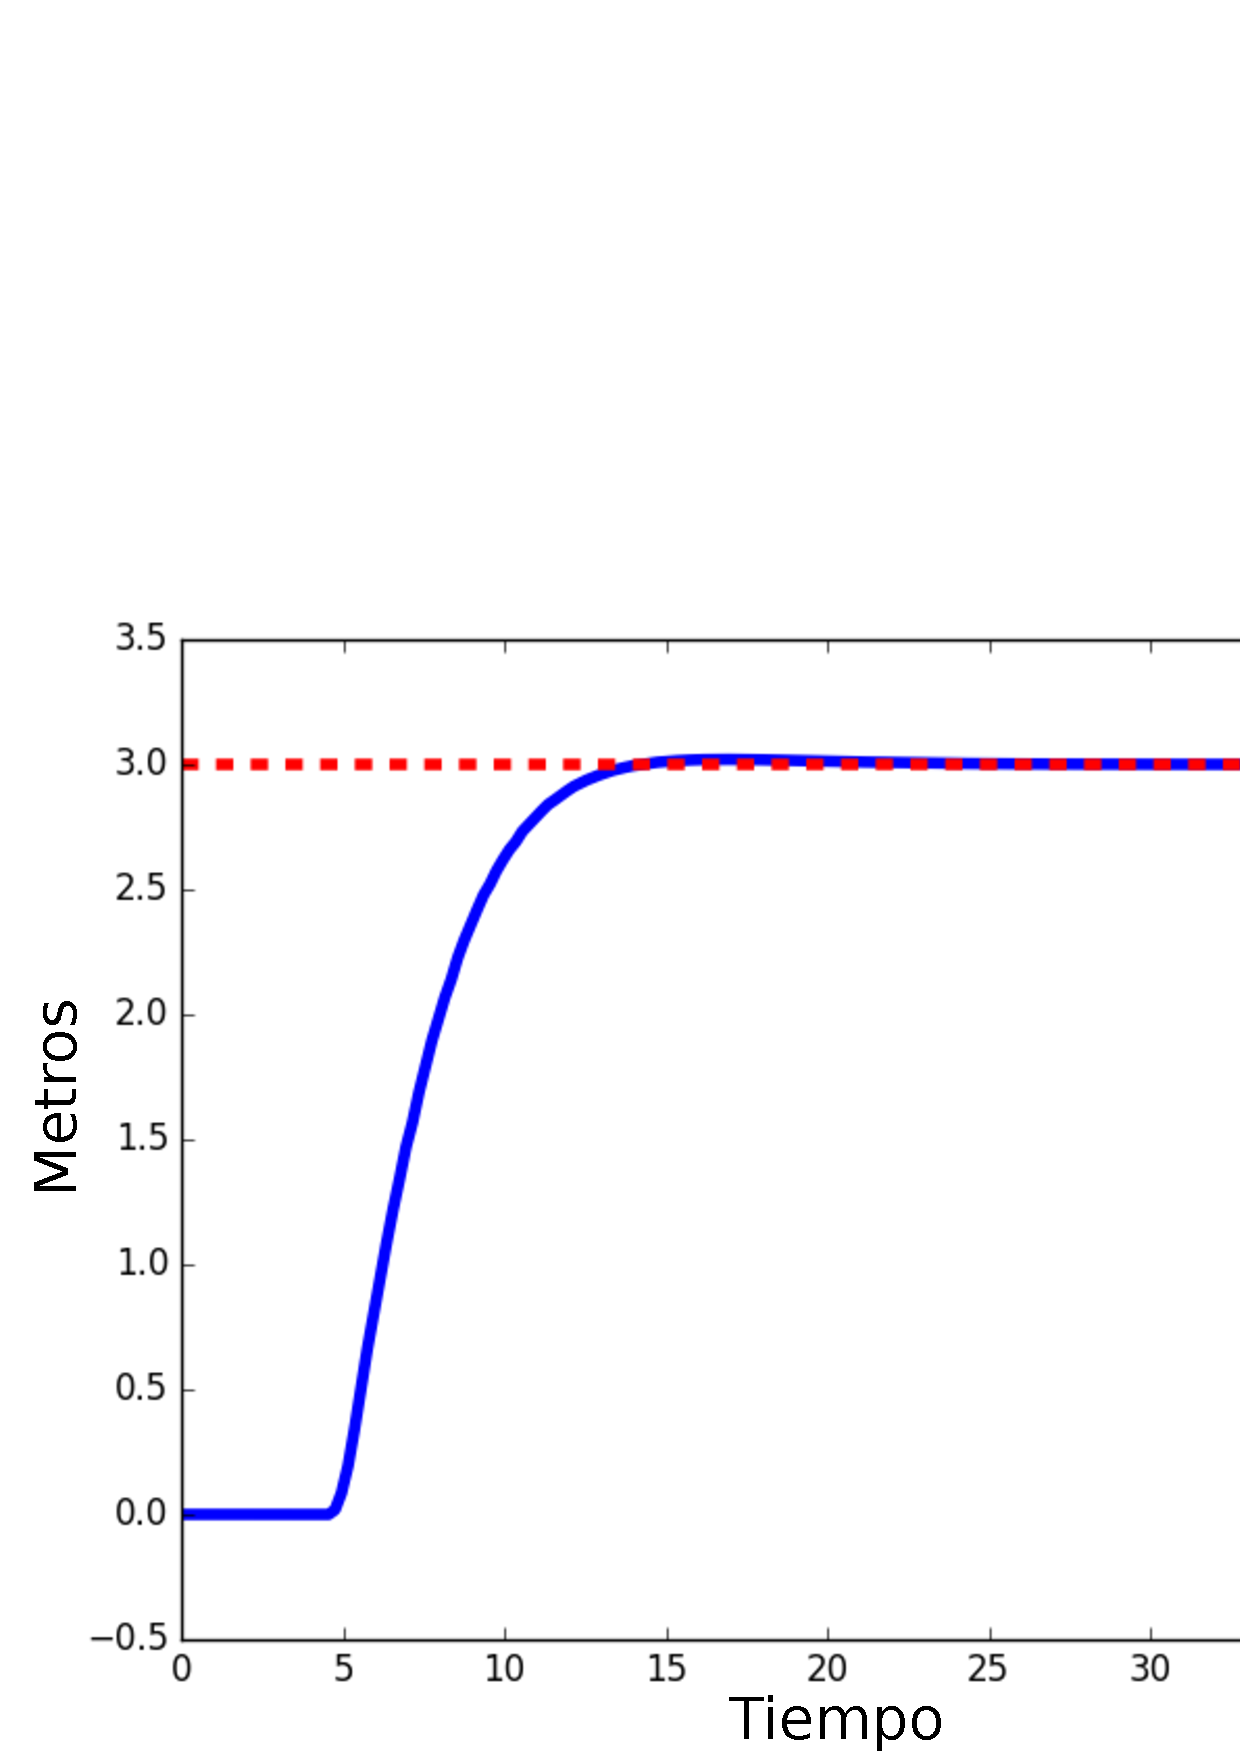
\includegraphics[width=.45\textwidth]{images/tvsxy_tesis.png}}
%        \subfigure[]{\label{fig:etiquetaB}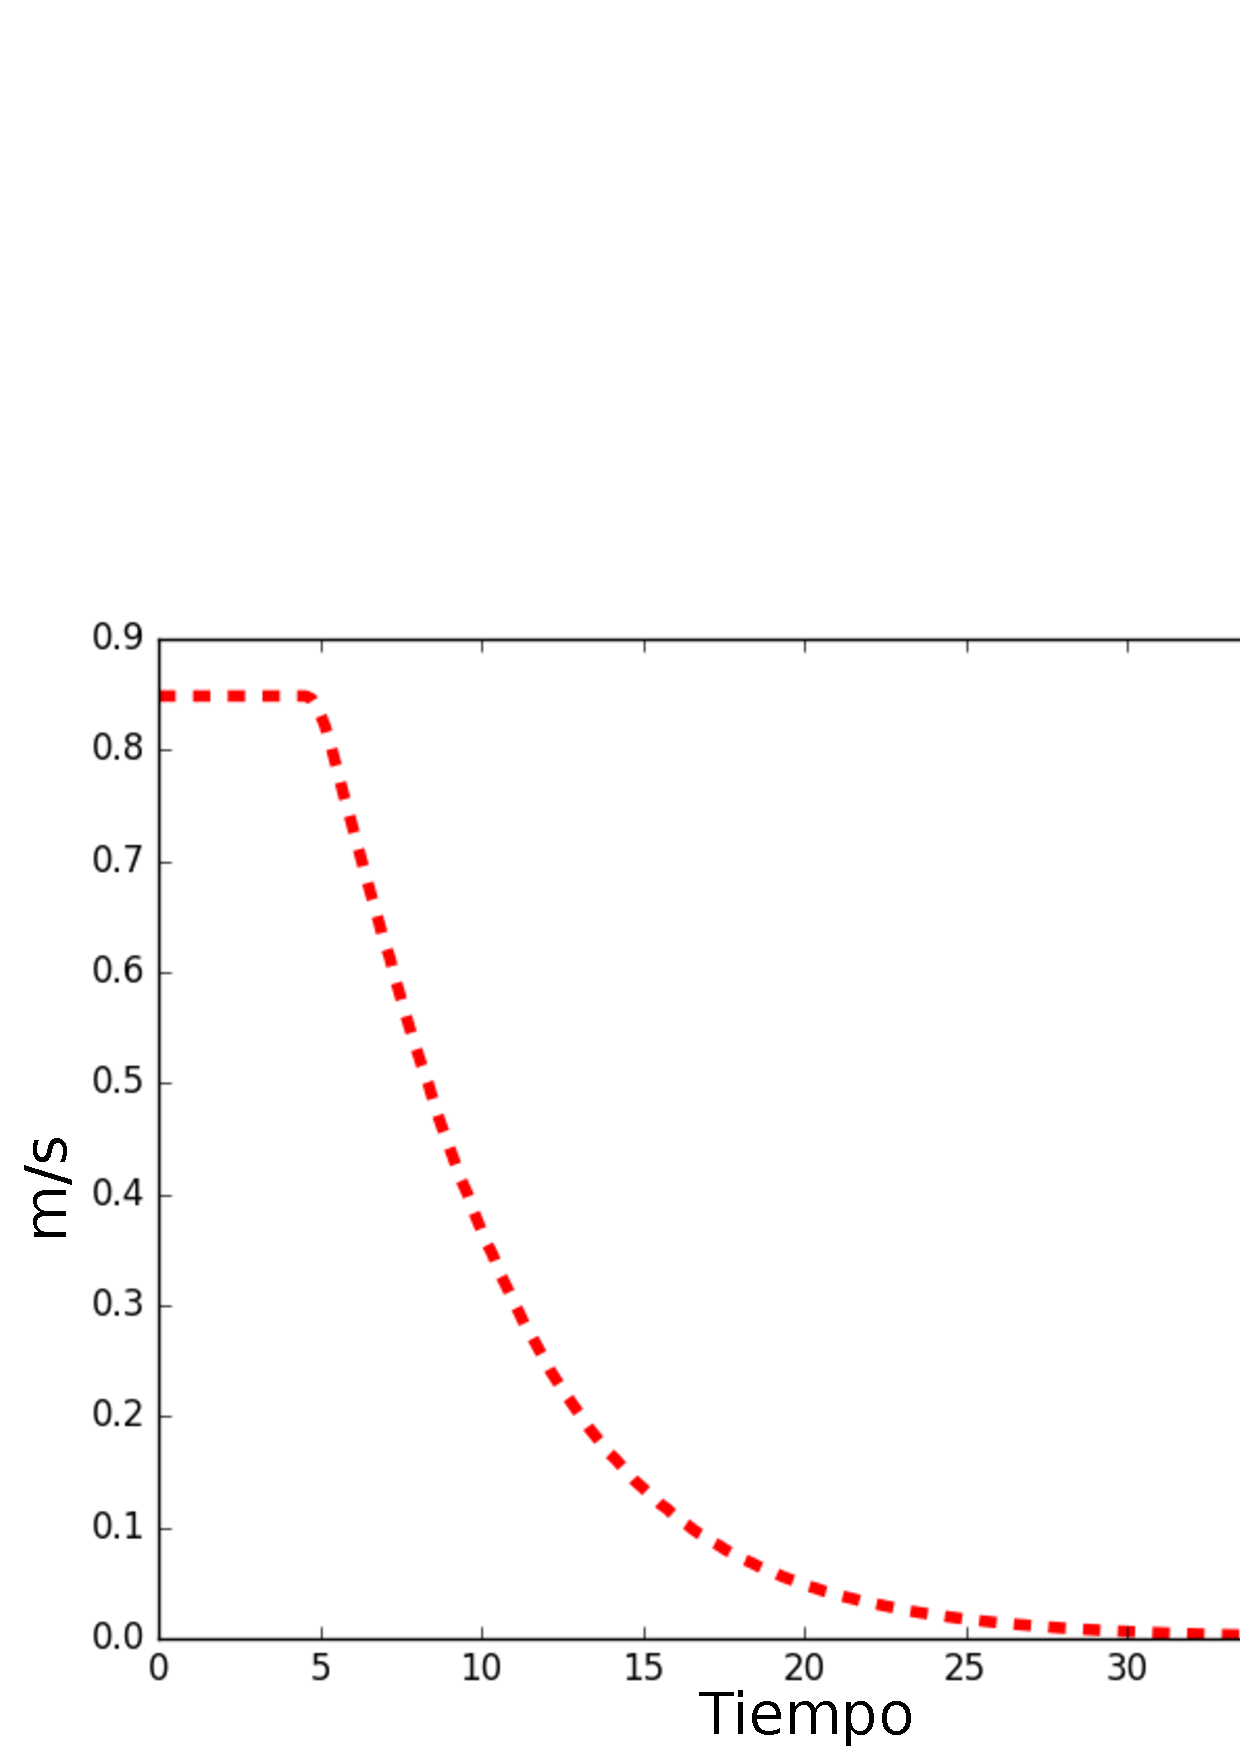
\includegraphics[width=.45\textwidth]{images/tvsv_tesis.png}}
%        \subfigure[]{\label{fig:etiquetaC}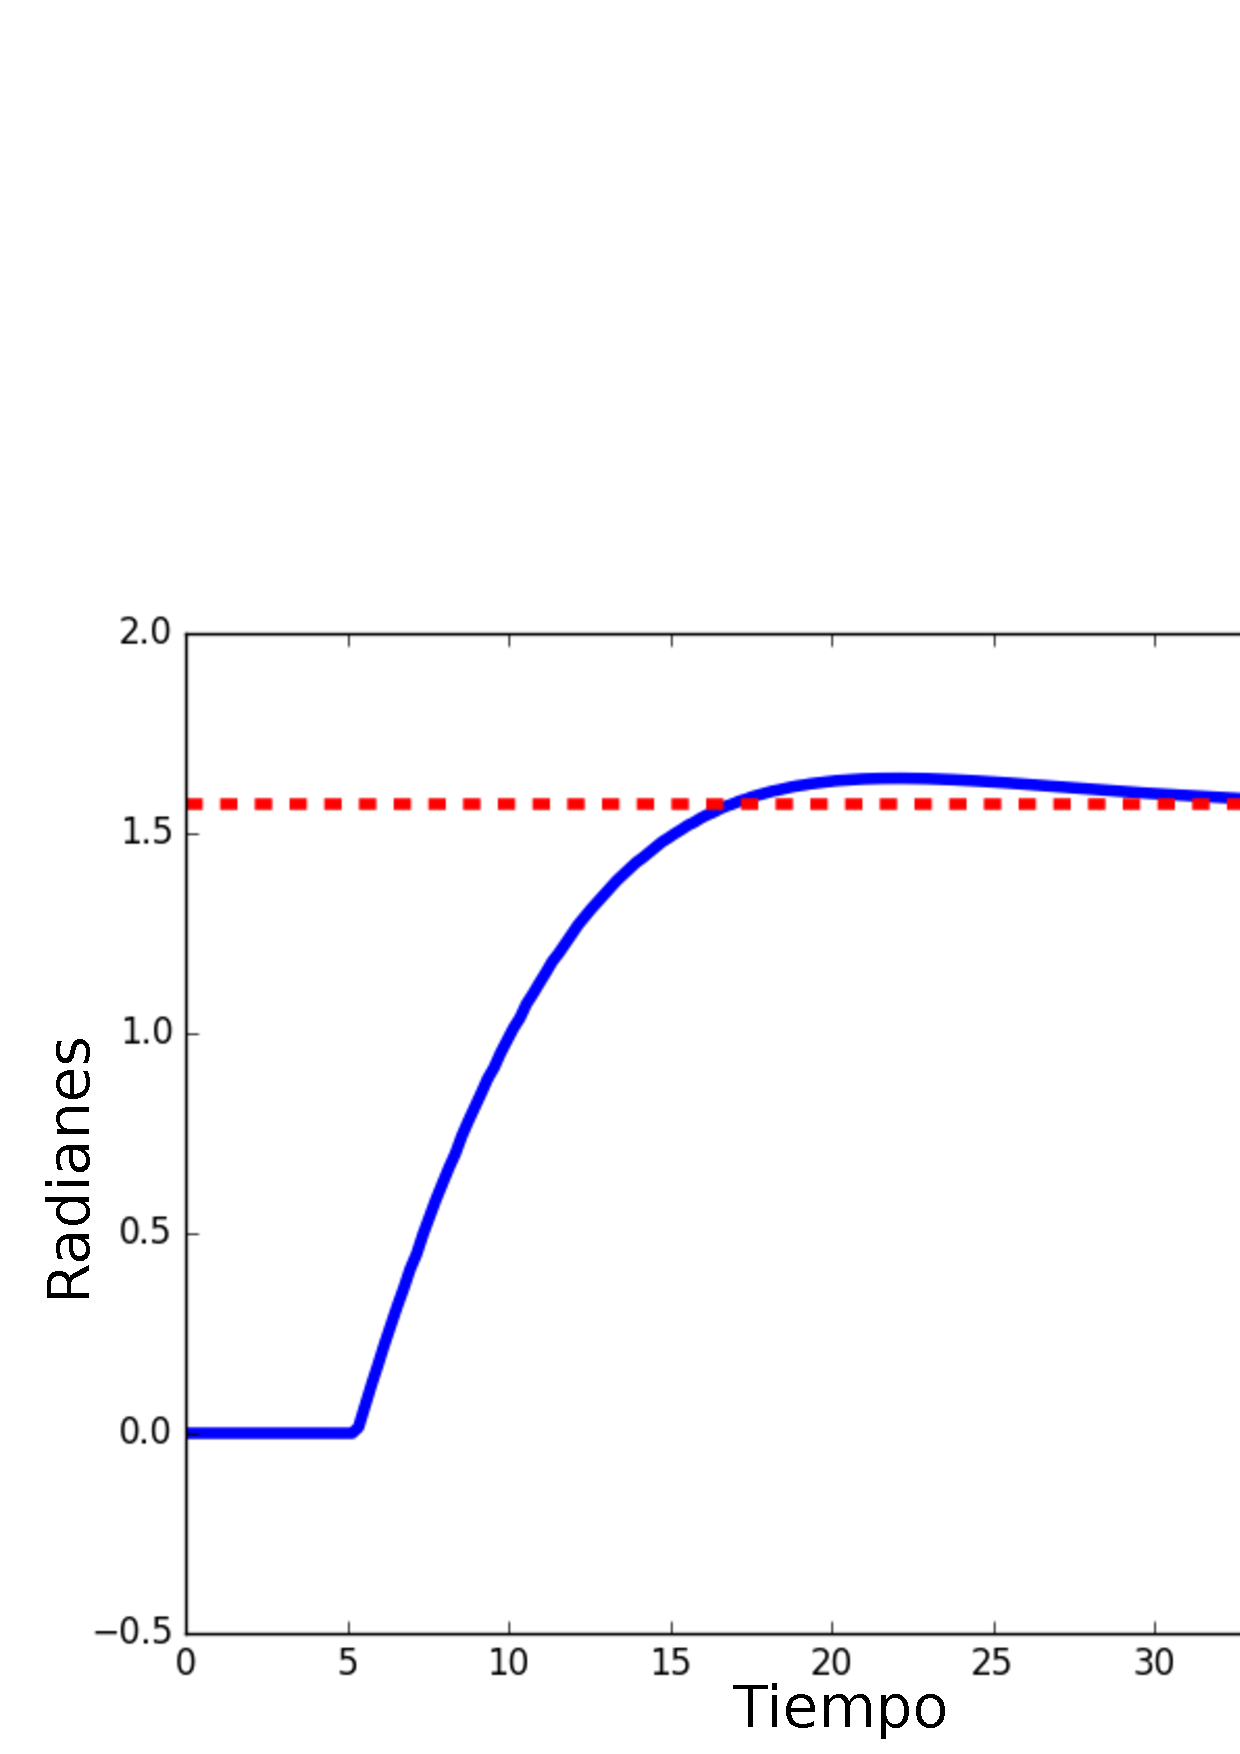
\includegraphics[width=.45\textwidth]{images/tvstheta_tesis.png}}
%        \subfigure[]{\label{fig:etiquetaD}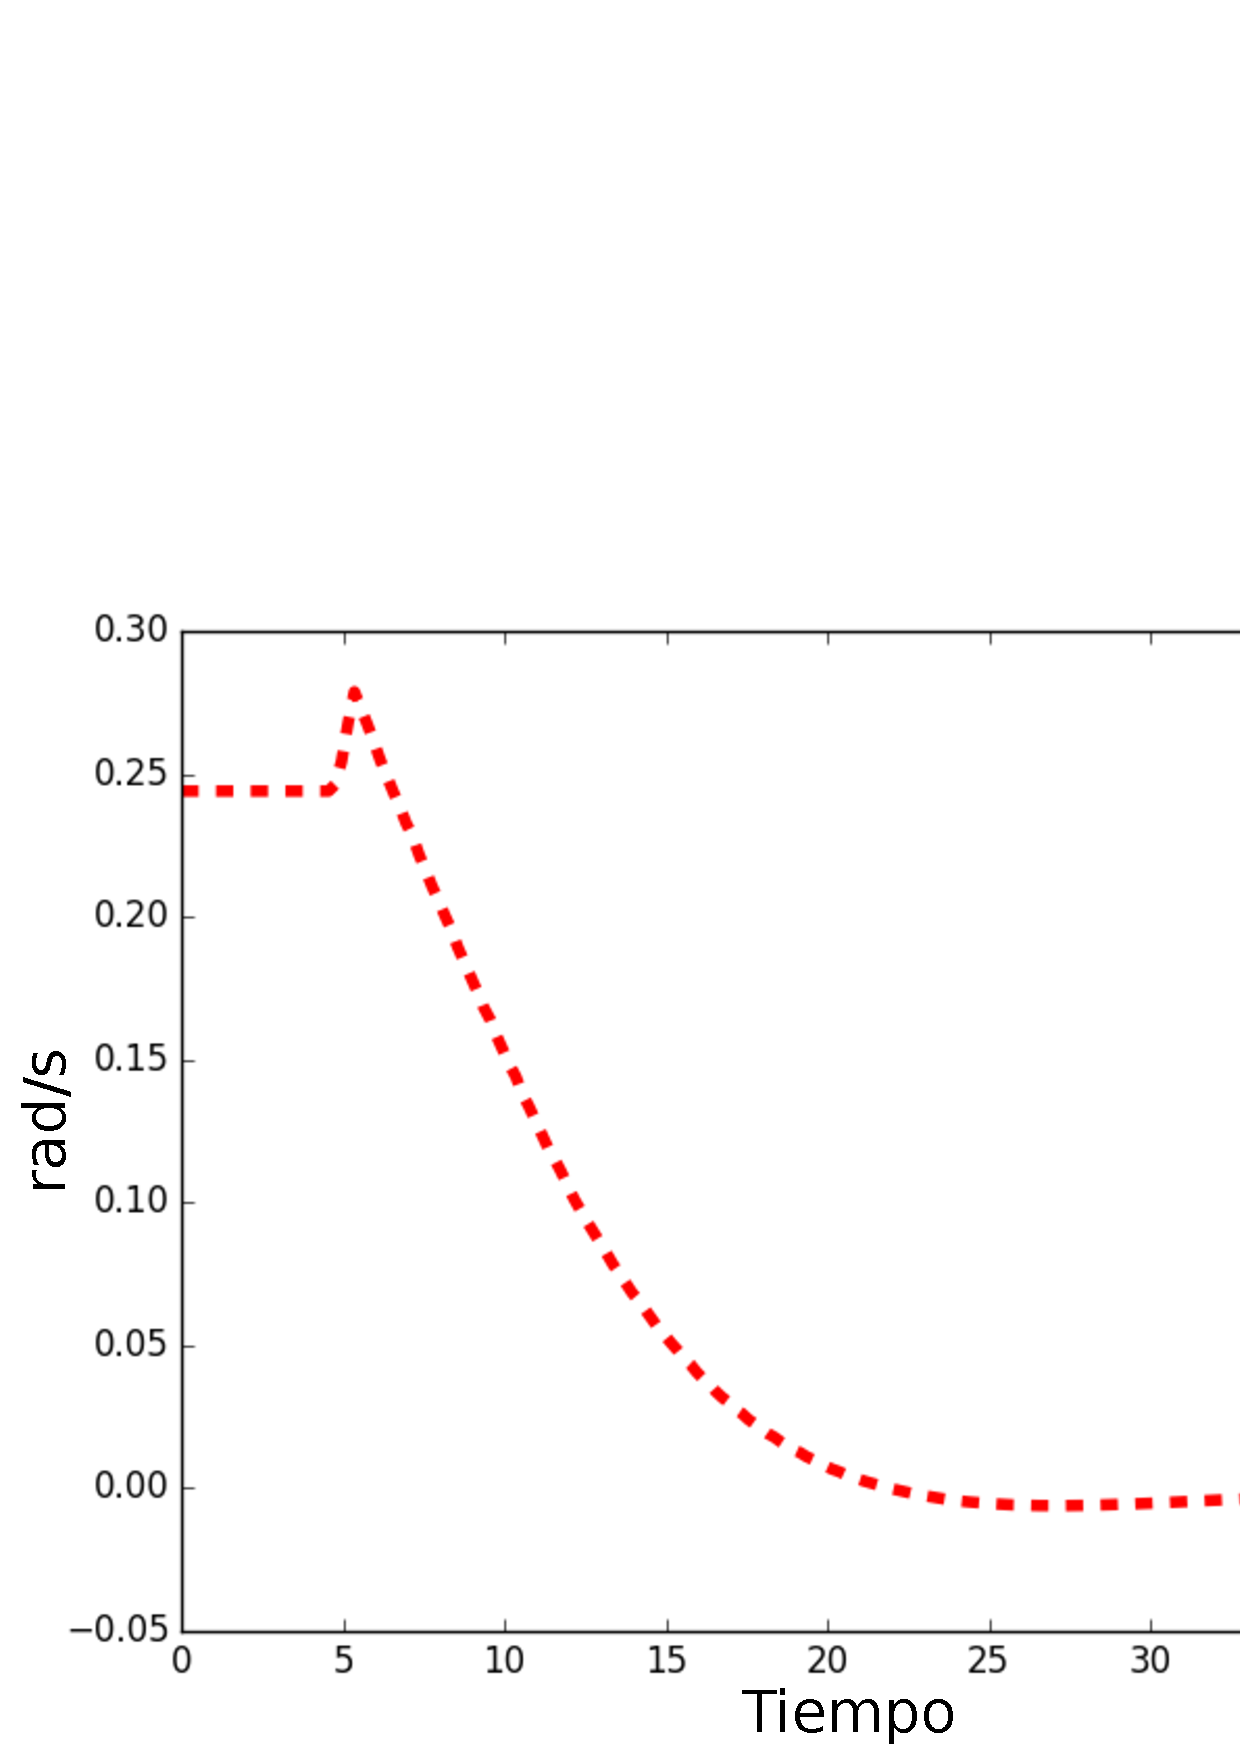
\includegraphics[width=.45\textwidth]{images/tvsomega_tesis.png}}
%    \end{center}
%  \captionsetup{font=footnotesize}
%    \caption{\label{f:PolarControl}Evolución temporal de las variables de estado usando el 
%    controlador polar para lograr una posición deseada dada por $x = 3, y = 3, 
%    \theta = 90$. En (a) se muestra la evolución temporal en la posición del eje x, en (b) 
%    se muestra la evolución de la velocidad lineal, en (c) se muestra la evolución de la
%    orientación y en (d) se muestra la evolución de la velocidad angular.}
%\end{figure}

\begin{figure}[ht!]
  \begin{tabular}{cc}
  %\centering
    %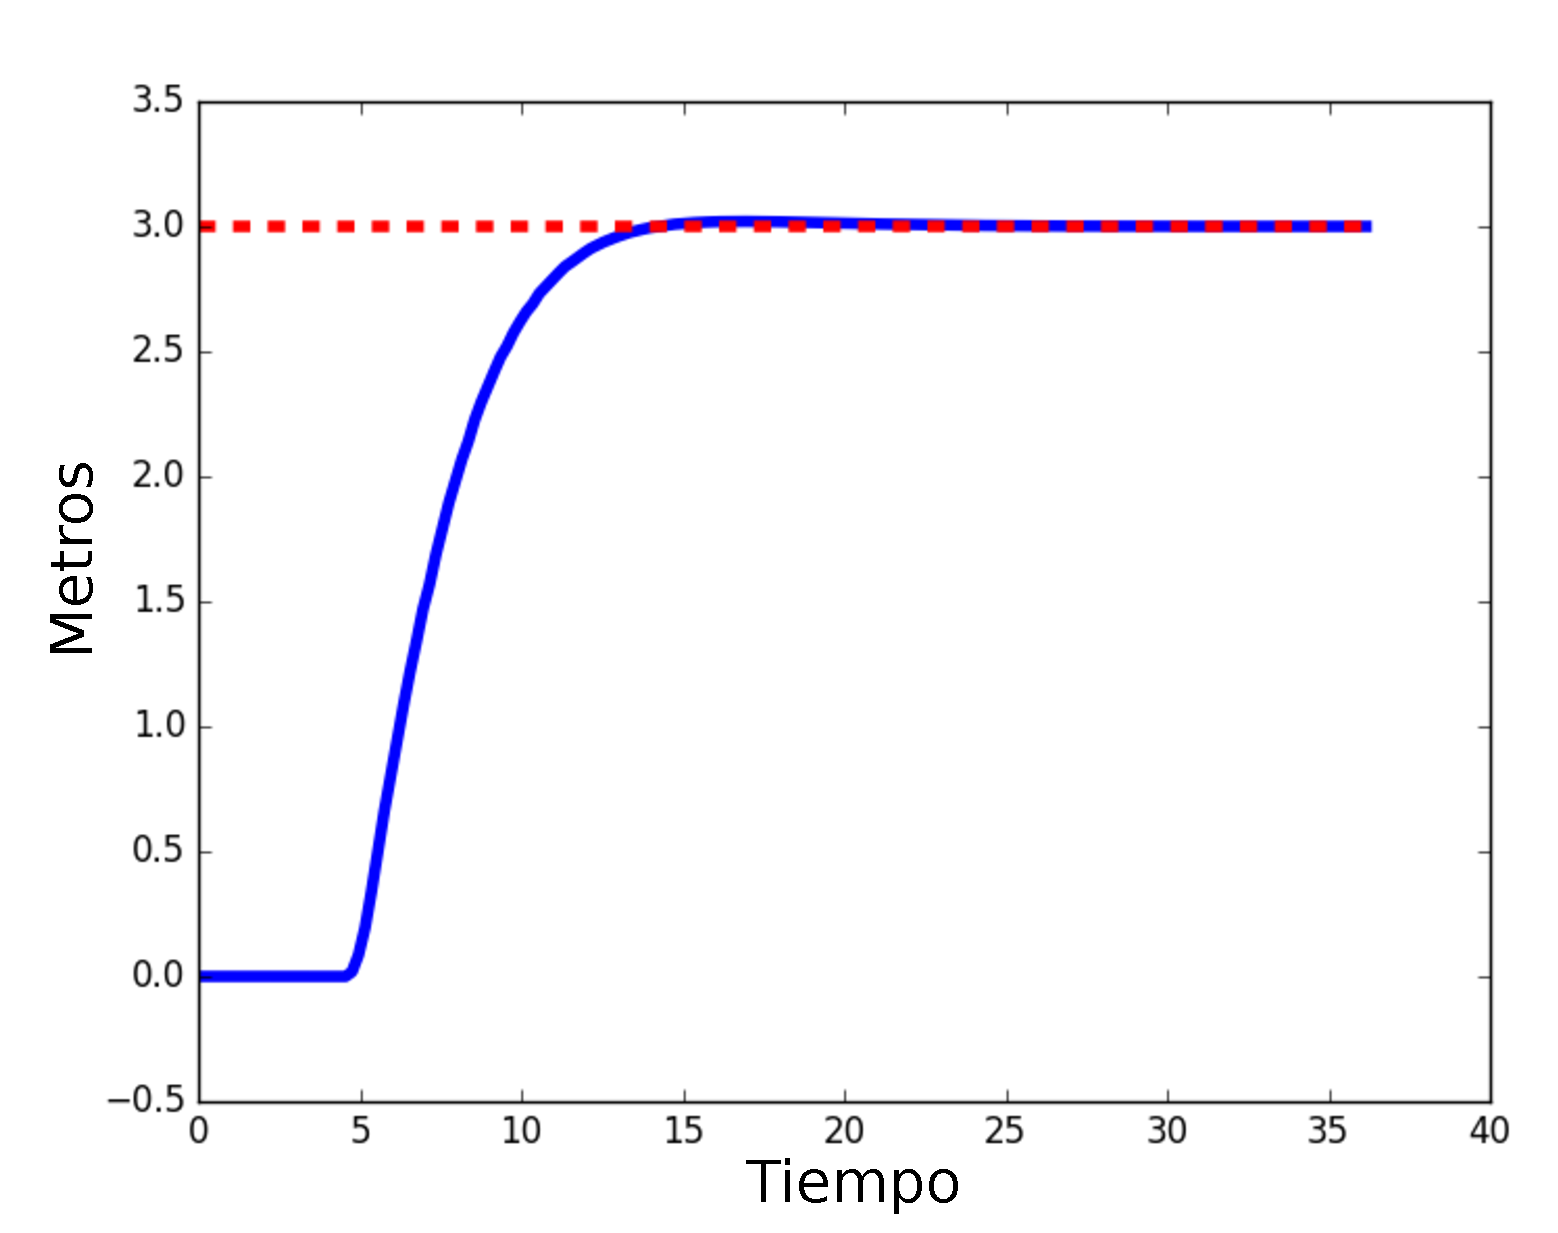
\includegraphics[width=.47\textwidth]{images/tvsxy_tesis.eps}&
    %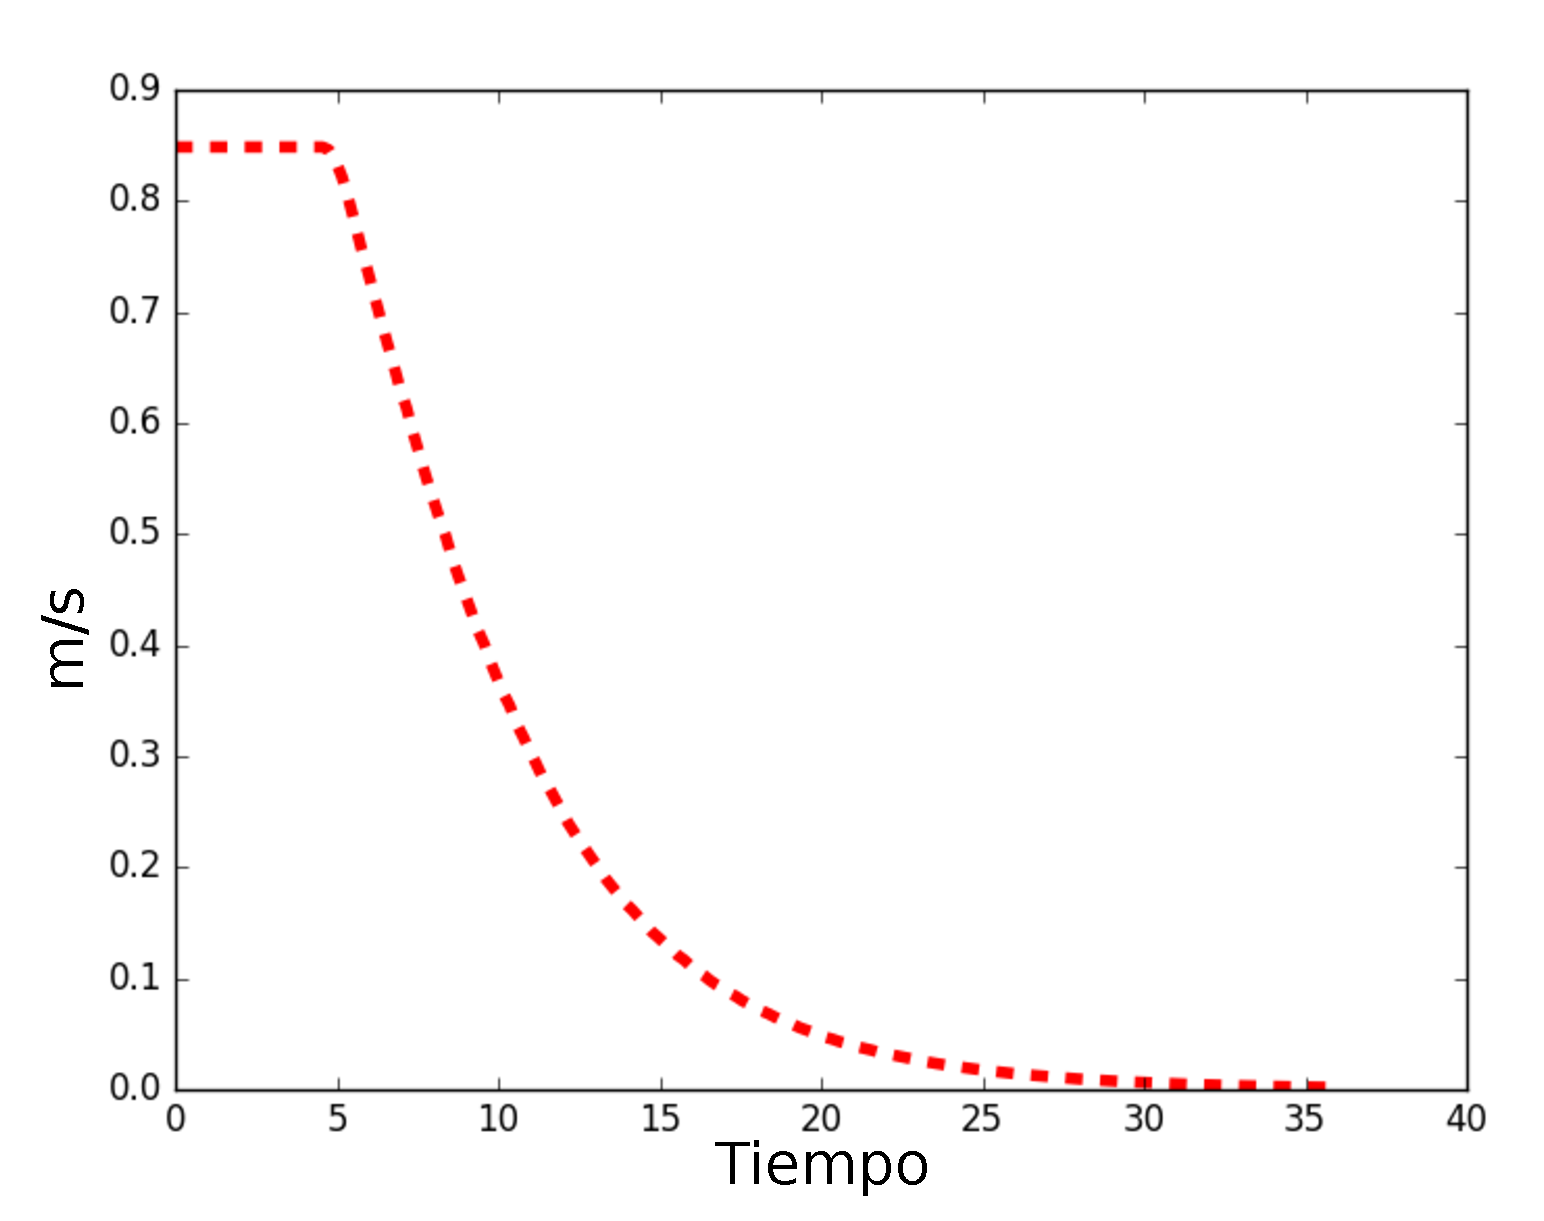
\includegraphics[width=.47\textwidth]{images/tvsv_tesis.eps}\\
    %(a)&(b)\\
    %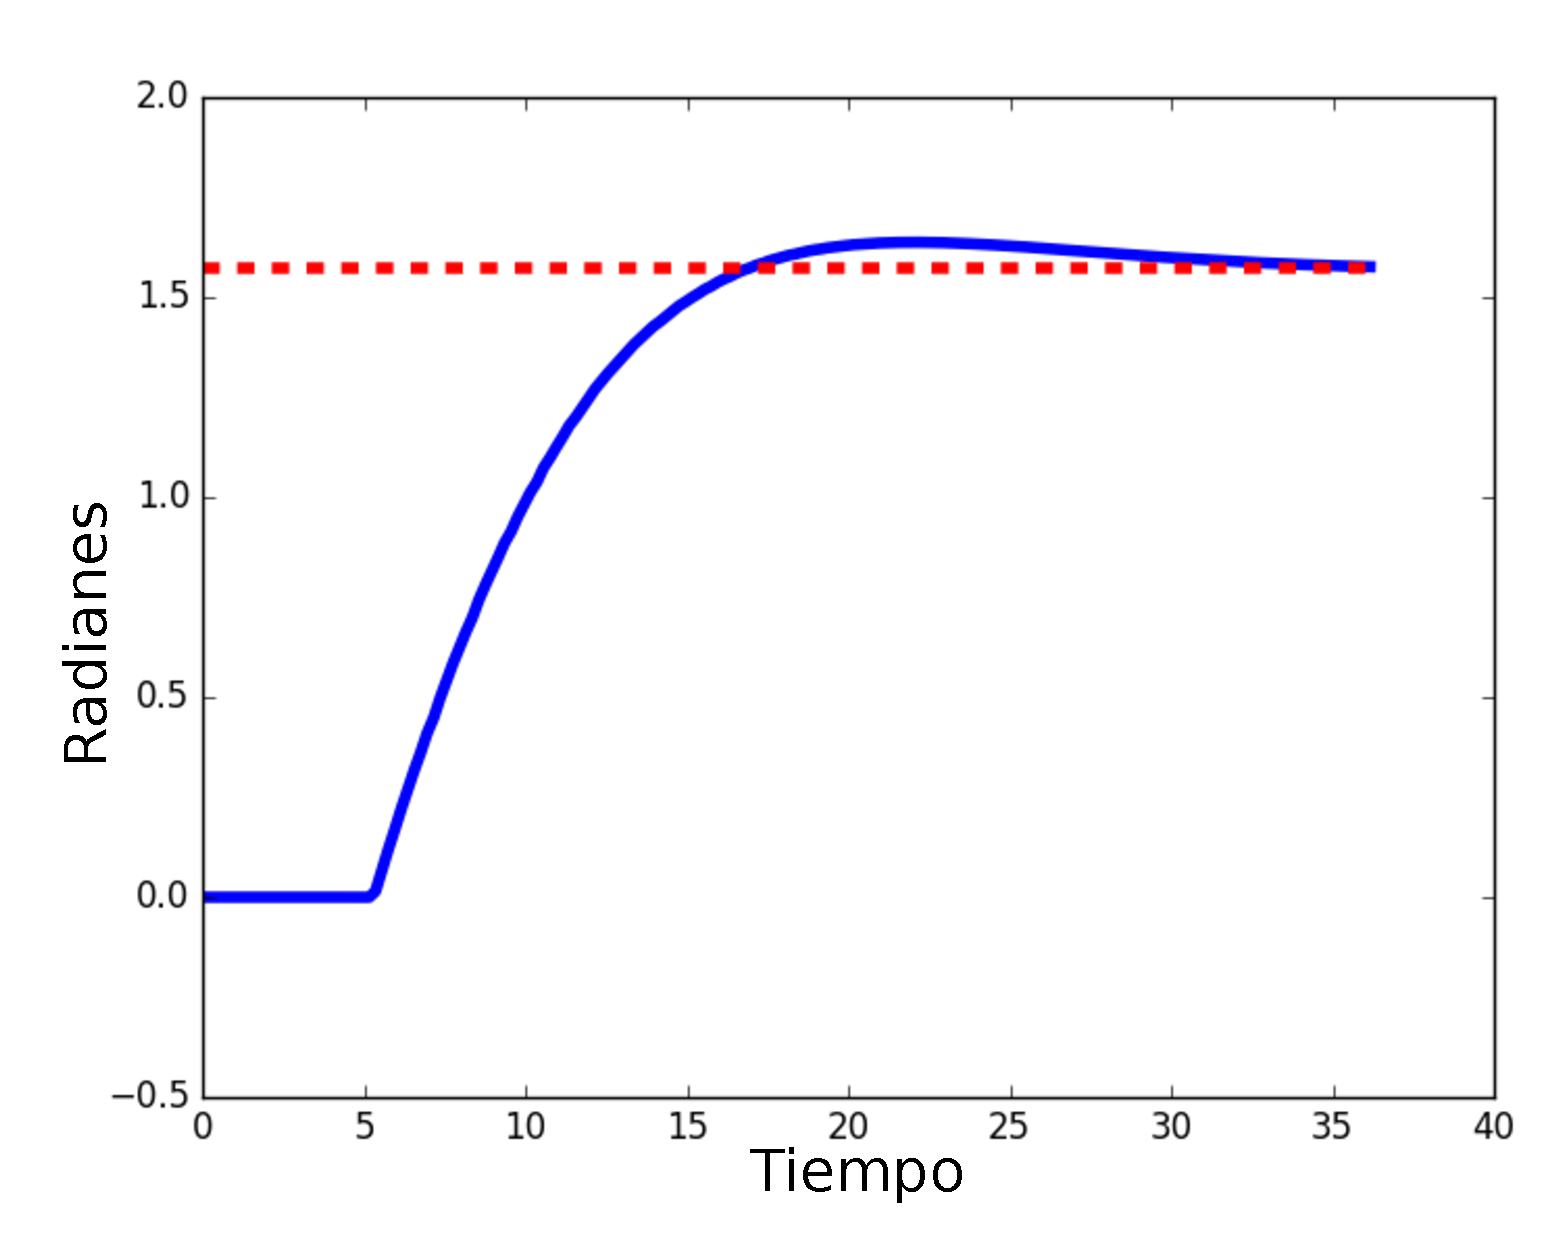
\includegraphics[width=.47\textwidth]{images/tvstheta_tesis.eps}&
    %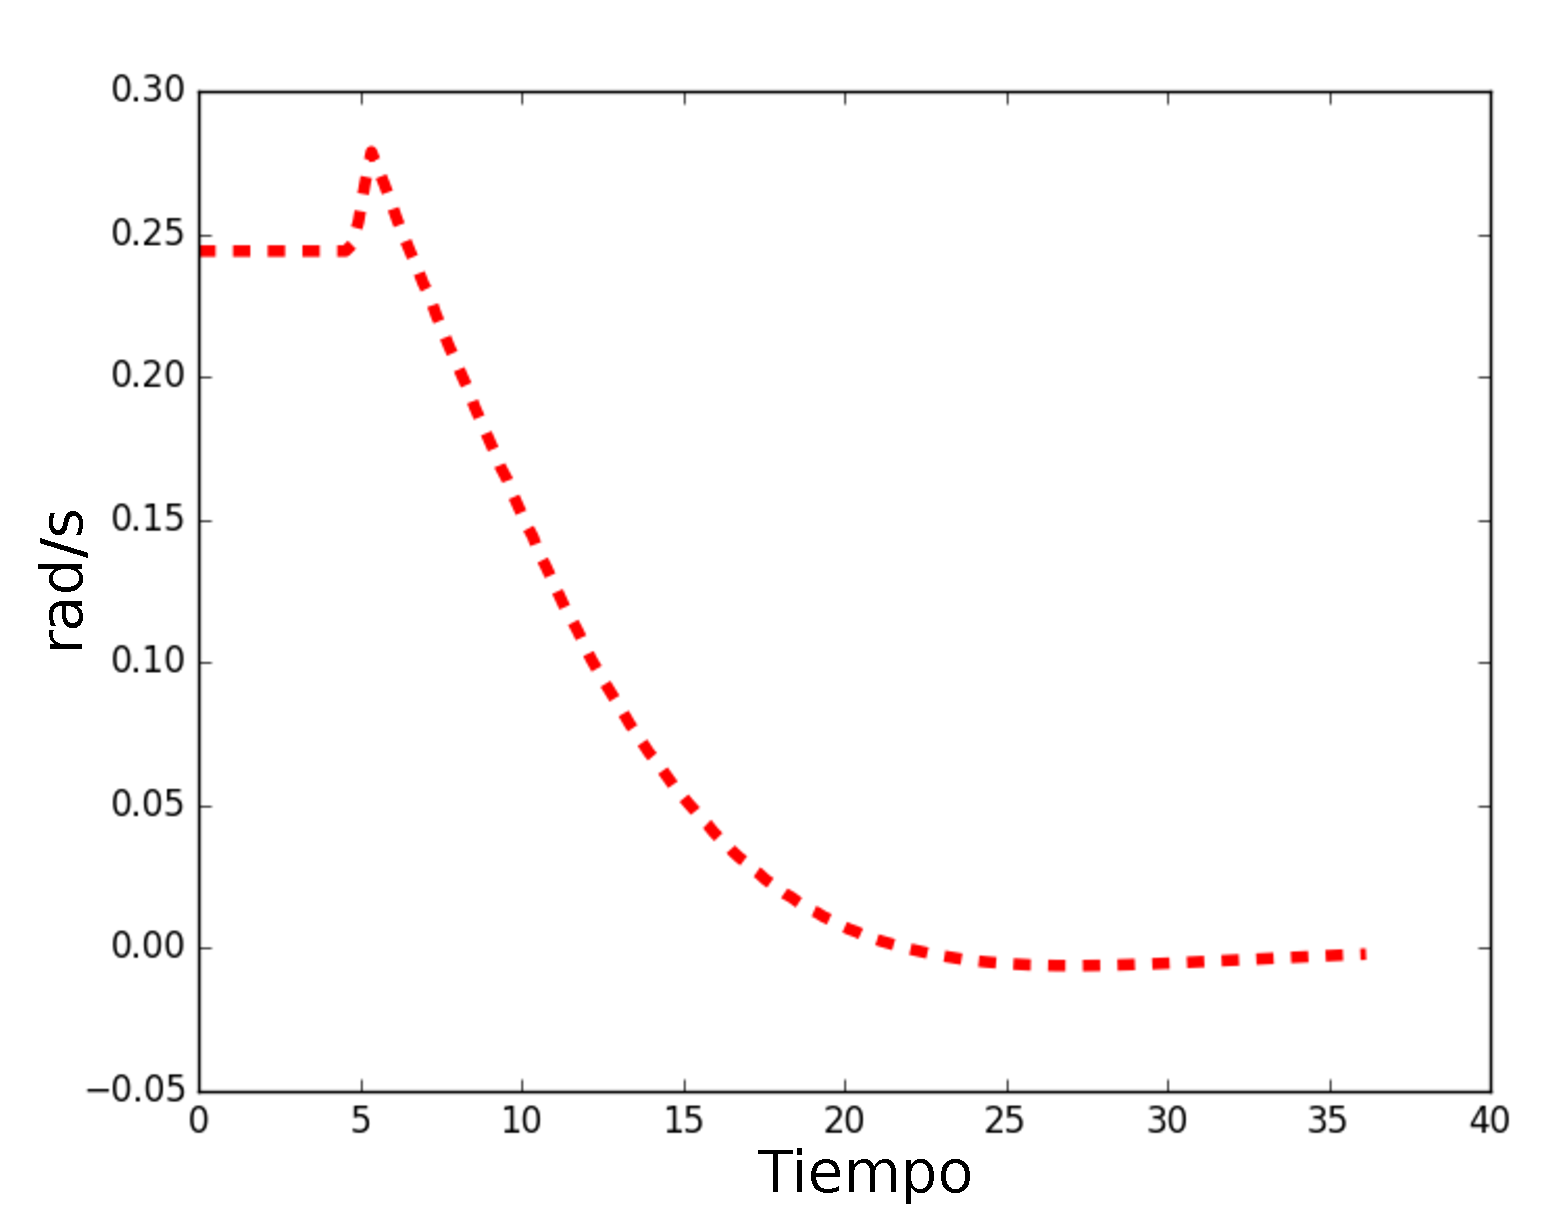
\includegraphics[width=.47\textwidth]{images/tvsomega_tesis.eps}\\
    %(c)&(d)
    \includegraphics[width=.47\textwidth]{images/PosicionEnX_tesis.PNG}&
    \includegraphics[width=.47\textwidth]{images/velocidadEnX_tesis.PNG}\\
    (a)&(b)\\
    \includegraphics[width=.47\textwidth]{images/orientacion_tesis.PNG}&
    \includegraphics[width=.47\textwidth]{images/velocidadAngular_tesis.PNG}\\
    (c)&(d)
  \end{tabular}
  \caption{Evolución temporal de las variables de estado usando el controlador polar para 
  lograr una posición deseada dada por $x = 3 m, y = 3 m, \theta = 90$. En (a) se muestra la 
  evolución temporal en la posición del eje x, en (b) se muestra la evolución de la 
  velocidad lineal, en (c) se muestra la evolución de la orientación y en (d) se muestra 
  la evolución de la velocidad angular.}
  \label{f:PolarControl}
\end{figure}


%\begin{figure}%[ht!]
%  \centering \footnotesize
%  \includegraphics[width=0.49\textwidth]{images/tvsxy_tesis.png}
%  \includegraphics[width=0.49\textwidth]{images/tvsv_tesis.png}
%  \includegraphics[width=0.49\textwidth]{images/tvstheta_tesis.png}
%  \includegraphics[width=0.49\textwidth]{images/tvsomega_tesis.png}
%  \captionsetup{font=footnotesize}
%  \caption{Evolución temporal de las variables de estado usando el controlador polar 
%  para lograr una posición deseada dada por $x = 3, y = 3, \theta = 90$}
%  \label{f:PolarControl}
%\end{figure}
Para probar el controlador polar, se usó una simulación dinámica en Gazebo con el robot 
Kobuki sin obstáculos, y las variables de estado que incluyen velocidad, posición y 
orientación se obtuvieron en línea a partir de la odometría simulada. Usando la información 
de esta odometría, el controlador se aplicó en línea. Para estas pruebas, la posición deseada
es $(x = 3 m, y = 3 m)$ y la orientación deseada $\theta = 90^{\circ}$. La Figura 
\ref{f:PolarControl}a muestra la evolución temporal de la posición ($x$) donde 
se logra una convergencia a la posición deseada en menos de 20 segundos. Esto se debe a 
la distancia hacia el obstáculo. Diferentes distancias conducen a diferentes tiempos de 
convergencia, y la tasa de convergencia también se puede modificar cambiando las 
ganancias en \ref{eqn:w} para la velocidad angular, y en \ref{eqn:v} para la velocidad 
lineal. Las otras subfiguras en la Figura \ref{f:PolarControl} muestran la evolución 
temporal de la velocidad lineal en $x$, la orientación y la velocidad angular. Para la 
orientación, hay un sobreimpulso que se debe a la excesiva dependencia del controlador 
en la posición en lugar de la orientación (ver Figura \ref{f:PolarControl}c).
%\section{An\'alisis del mapa obtenido}
%\section{Resultados en un ambiente real}
\section{Resultados del Sistema de Navegación}
\begin{figure}%[ht!]
  \centering
  \begin{tabular}{cc}
      %\subfigure[Fuerzas de atracción aplicado al robot móvil]{\label{fig:etiquetaA}\includegraphics
      %[width=.49\textwidth]{images/attr_kbki.eps}}
     \includegraphics[width=0.51\linewidth]{images/attr_kbki.eps}&
      %\subfigure[Fuerzas de repulsión aplicado al robot móvil]{\label{fig:etiquetaB}\includegraphics
      %[width=.49\textwidth]{images/rep_kbki.eps}}
     \includegraphics[width=0.51\linewidth]{images/rep_kbki.eps}\\
    (a) & (b)\\
    \multicolumn{2}{c}{\includegraphics[width=0.52\linewidth]{images/nav_kbki.eps}}\\
      %\subfigure[Fuerzas de navegación aplicado al robot móvil]{\label{fig:etiquetaC}\includegraphics
      %[width=.49\textwidth]{images/nav_kbki.eps}}
    \multicolumn{2}{c}{(c)}
  \end{tabular}
 
  \caption{Navegación autónoma implementada en el robot diferencial Kobuki. En (a) se muestra
  las fuerzas de atracción que llevan al Kobuki a la posición deseada, en (b) se muestra las 
  fuerzas de repulsión que evitan que el robot diferencial se choque con los obstáculos y en 
  (c) se muestra las fuerzas de navegación que genera la trayectoria del robot.}
  \label{f:kbki_APF}
 \end{figure}
%\begin{figure}%[ht!]
%  \centering \footnotesize
%  \includegraphics[width=0.61\textwidth]{images/attr_kbki.png}
%  \includegraphics[width=0.60\textwidth]{images/rep_kbki.png}
%  \includegraphics[width=0.60\textwidth]{images/nav_kbki.png}
%  \captionsetup{font=footnotesize}
%  \caption{Navegación autónoma implementada en el robot diferencial Kobuki.}
%  \label{f:kbki_APF}
%\end{figure}
La metodología propuesta se implementó como un algoritmo iterativo en el robot Kobuki. 
Como se describe en la sección \ref{sec:autonomia}, el algoritmo toma iterativamente 
posiciones deseadas  donde a través del campo potencial artificial y el controlador 
polar impulsan al robot a través de las posiciones requeridas. Se expuso al robot 
a diferentes obstáculos cuyas posiciones fueron conocidas a priori. La Figura \ref{f:kbki_APF} muestra un ejemplo de aplicación del sistema de navegación. La Figura 
\ref{f:kbki_APF}a muestra las fuerzas de atracción para cada posición (puntos rojos) en 
las que el algoritmo se itera en el entorno de dos dimensiones dentro del movimiento del 
robot. Para cada posición, el campo de potencial atractivo se puede ver con la dirección 
de las flechas. La Figura \ref{f:kbki_APF}b se compone de las fuerzas de repulsión basadas en 
los obstáculos que se muestran como marcadores verdes. Para cada obstáculo, la magnitud de 
las fuerzas aumenta cuando el robot está más cerca y su dirección señala los obstáculos, permitiendo 
que el robot los evite. La Figura \ref{f:kbki_APF}c muestra la superposición de ambas fuerzas 
con los obstáculos reales. Cada fuerza proporciona una posición deseada intermedia para el 
robot, que constituye la posición deseada continuamente actualizada para el controlador 
polar. Aunque las fuerzas cercanas a los obstáculos tienen un alto índice de cambio, la 
trayectoria es suave. Esto demuestra la efectividad del sistema de navegación a pesar de las 
características no holonómicas del robot.

\section{Resultados de la Navegación Autónoma con el Lídar en dos dimensiones}
\begin{figure}%[ht!]
  \centering \footnotesize
  \includegraphics[width=0.80\textwidth]{images/kobuki_201.jpg}
  \captionsetup{font=footnotesize}
  \caption{Navegación autónoma del robot diferencial Kobuki, montado con un 
  sensor lídar y dos cajas como obstáculos.}
  \label{fig:Kobuki201}
\end{figure}

%\begin{figure}[ht!]
%     \begin{center}
%        \subfigure[Fuerzas de atracción aplicado al robot móvil]{\label{fig:etiquetaA}\includegraphics
%        [width=.69\textwidth]{images/fattr_lidar_s.eps}}
%        \subfigure[Fuerzas de repulsión aplicado al robot móvil]{\label{fig:etiquetaB}\includegraphics
%        [width=.69\textwidth]{images/frep_lidar_s.png}}
%        \subfigure[Fuerzas de navegación aplicado al robot móvil]{\label{fig:etiquetaC}\includegraphics
%        [width=.69\textwidth]{images/fnav_lidar_s.png}}
%    \end{center}
\begin{figure}
  \centering
    \begin{tabular}{c}
      \multicolumn{1}{c}{\includegraphics[width=.75\textwidth]{images/fattr_lidar_s.eps}}\\
      \multicolumn{1}{c}{(a)}\\
      \multicolumn{1}{c}{\includegraphics[width=.75\textwidth]{images/frep_lidar_s.eps}}\\
      \multicolumn{1}{c}{(b)}\\
      \multicolumn{1}{c}{\includegraphics[width=.75\textwidth]{images/fnav_lidar_s.eps}}\\
      \multicolumn{1}{c}{(c)}
    \end{tabular}
  \captionsetup{font=footnotesize}
    \caption{\label{f:kbki_autonomo}Campos atractivos y repulsivos, y la trayectoria que el 
    robot real sigue usando datos en línea provenientes del sensor lídar montado en la parte 
    superior. En (a) se muestra las fuerzas de atracción, en (b) las fuerzas de repulsión y 
    las posiciones de los obsáculos, finalmente en (c) se muestra las fuerzas de navegación 
    generando la trayectoria.}
\end{figure}

%\begin{figure}%[ht!]
%  \centering \footnotesize
%  \includegraphics[width=0.80\textwidth]{images/fattr_lidar_s.png}
%  \includegraphics[width=0.80\textwidth]{images/frep_lidar_s.png}
%  \includegraphics[width=0.80\textwidth]{images/fnav_lidar_s.png}
%  \captionsetup{font=footnotesize}
%  \caption{Campos atractivos y repulsivos, y la trayectoria que el robot real sigue 
%  usando datos en línea provenientes del sensor lidar montado en la parte superior.}
%  \label{f:kbki_autonomo}
%\end{figure}

Para probar la autonomía del robot móvil en un entorno real, se usa un sensor lídar 
(RPLidar A2) que se colocó sobre el robot Kobuki. Se usa el sensor lídar para poder 
hacer una actualización continua de las posiciones de los obstáculos a medida que el 
robot se mueve. El robot usa tópicos creados en ROS para obtener la información del 
sensor, la cual se compone en rango y orientación por cada punto medido, a medida que 
el sensor lídar gira. La información del lídar se tuvo que convertir a coordenadas 
cartesianas para conocer las posiciones de cada obstáculo dentro del 
espacio de trabajo. Estas posiciones van como entrada hacia el algoritmo principal. 
El robot Kobuki puede desplazarse dentro del mapa generado por el lídar, para que esto
ocurra se tuvo que considerar el marco de referencia del robot como el marco de 
referencia del sensor lídar. Entonces, el algoritmo de navegación autónomo usa 
las coordenadas del entorno detectados mediante el sensor lídar y así genera su propia 
trayectoria evitando los obstáculos del entorno. Para una prueba, se colocaron dos 
cajas en el espacio de trabajo, como se ve en la Figura \ref{fig:Kobuki201}. La posición 
del objetivo era ($x = 4 m, y = 0 m$) y la posición donde inició el robot fue 
($x = 0 m, y = 0 m$). La Figura \ref{f:kbki_autonomo}a muestra la trayectoria del robot 
en azul y las flechas indican la fuerza de atracción que llevan al robot hacia la 
posición deseada. La Figura \ref{f:kbki_autonomo}b muestra el mapa completo, donde 
los puntos verdes representan el entorno y los obstáculos del entorno, detectados por 
el lídar, donde se mueve el robot. En este caso los obstáculos del entorno son las 
dos cajas mostradas en la Figura \ref{fig:Kobuki201} y que se muestran muy cercanas 
a la trayectoria formada por el robot en la Figura \ref{f:kbki_autonomo}b. Como se 
observa, estas flechas apuntan hacia afuera del obstáculo, proporcionando autonomía 
al robot mientras intenta alcanzar la posición deseada. Estas flechas representan 
a las fuerzas de repulsión, que evitan la colisión entre el robot y los obstáculos 
del entorno. Finalmente en la Figura \ref{f:kbki_autonomo}c se muestra toda la 
fuerza de navegación que impulsa el movimiento del robot móvil, asimismo esta fuerza 
genera la trayectoria representada por los puntos de color azul. La forma de la trayectoria
es debido a las dos cajas que se encuentran entre la posición inicial y la posición final.

\section{Resultado de la Navegación Autónoma usando SLAM en dos dimensiones}
\begin{figure}%[ht!]
  \centering \footnotesize
  %\includegraphics[width=0.80\textwidth]{images/gazebo_map.png}
  \includegraphics[width=0.80\textwidth]{images/kbki_ambient.png}
  \captionsetup{font=footnotesize}
  \caption{Robot móvil Kobuki en medio de los obstáculos colocados para probar la 
  navegación autónoma utilizando el algoritmo SLAM. Esta prueba se realizó en el
  simulador Gazebo.}
  \label{fig:Gazebo_simu}
\end{figure}
Para probar la navegación autónoma del robot Kobuki usando el algoritmo SLAM, se utilizó
el simulador dinámico Gazebo. En este simulador se creó un escenario donde se colocó al 
robot Kobuki en medio de varios obstáculos. Los obstáculos fueron colocados de tal forma
que pueda representar la entrada de un túnel. En la Figura \ref{fig:Gazebo_simu} se puede
ver el escenario que fue creado. Un conjunto de obstáculos tiene una longitud de 3 metros
y el ancho entre los conjuntos de obstáculos es de 4 metros. El robot tiene que desplazarse
por ese espacio hasta llegar a la posición deseada, estimar la posición de los obstáculos 
y construir el mapa en dos dimensiones.

\begin{figure}%[ht!]
     %\begin{center}
     %   \subfigure[Fuerzas de atracción aplicado al robot móvil en tiempo real]{\label{fig:etiquetaA}\includegraphics
     %   [width=.69\textwidth]{images/fattr_slam.png}}
     %   \subfigure[Fuerzas de repulsión aplicado al robot móvil en tiempo real]{\label{fig:etiquetaB}\includegraphics
     %   [width=.69\textwidth]{images/frep_slam.png}}
     %   \subfigure[Fuerzas de navegación aplicado al robot móvil en tiempo real]{\label{fig:etiquetaC}\includegraphics
     %   [width=.69\textwidth]{images/fnav_slam.png}}
    %\end{center}
    \centering
    \begin{tabular}{c}
      \multicolumn{1}{c}{\includegraphics[width=.77\textwidth]{images/fattr_slam.eps}}\\
      \multicolumn{1}{c}{(a)}\\
      \multicolumn{1}{c}{\includegraphics[width=.77\textwidth]{images/frep_slam.eps}}\\
      \multicolumn{1}{c}{(b)}\\
      \multicolumn{1}{c}{\includegraphics[width=.77\textwidth]{images/fnav_slam.eps}}\\
      \multicolumn{1}{c}{(c)}
    \end{tabular}
  \captionsetup{font=footnotesize}
    \caption{\label{fig:Kbki_slam}Navegación autónoma del Kobuki utilizando
    SLAM. En (a) se muestra las fuerzas de atracción, en (b) se representa 
    las fuerzas de repulsión y en (c) la suma de las fuerzas de atracción y 
    repulsión.}
\end{figure}

%\begin{figure}%[ht!]
%  \centering \footnotesize
%  \includegraphics[width=0.80\textwidth]{images/fattr_slam.png}
%  \includegraphics[width=0.80\textwidth]{images/frep_slam.png}
%  \includegraphics[width=0.80\textwidth]{images/fnav_slam.png}
%  \captionsetup{font=footnotesize}
%  \caption{Campos atractivos y repulsivos, y la trayectoria que el robot real sigue 
%  usando datos en línea provenientes del sensor lidar montado en la parte superior del 
%  Kobuki.}
%  \label{fig:Kbki_slam}
%\end{figure}

Como se mencionó en la sección \ref{sec:GMAPPING}, para realizar esta prueba se utilizó
el paquete de SLAM llamado \textit{gmapping}, dado por ROS. Este paquete permite crear 
un mapa en dos dimensiones a partir de los datos del sensor lídar y la odometría del 
robot móvil. Cuando se ejecuta el paquete de SLAM, empieza a crear tópicos por donde se
envían los datos de la odometría del robot y los datos del lídar. Con la información 
recibida por el nodo del \textit{gmapping}, éste publica las dimensiones del entorno, dentro
de un tópico, hacia el robot Kobuki. Para que el robot móvil se pueda desplazar con respecto
a las dimensiones del mapa recibido por el SLAM, su marco de referencia debe ser remplazado
por el marco de referencia del sensor lídar. La precisión del mapa originado por el SLAM es 
buena, debido a que el algoritmo reduce la cantidad de mediciones que envía el sensor lídar
haciendo que el mapa sea uniforme y los obstáculos se encuentren en la posición correcta
dentro del mapa.

%Al momento de iniciar el paquete \textit{gmapping}, 
%este crea tópicos a los cuales se debe enviar los datos de la odometría del robot y los datos 
%del sensor lidar. Con la información dada el nodo de SLAM publica las dimensiones del mapa 
%dentro de un tópico. Para que el Kobuki se mueva con respecto al mapa generado, el marco de 
%referencia del Kobuki se toma como el marco de referencia del sensor lidar. El nodo de 
%SLAM tiene un alcance máximo de mapeo de 8 metros, tiene un tamaño de mapa en píxeles de 
%512 x 512 y una resolución de mapa de 2.5 centímetros por cada celda del mapa. Además el 
%algoritmo muestrea la cantidad de mediciones que envía el lidar, por tal motivo el mapa 
%obtenido es bastante uniforme y preciso con respecto a las posiciones de los obstáculos 
%dentro del mapa. 
Para el desplazamiento autónomo del robot, dentro del escenario creado, se utilizó las 
etapas de localización y mapeo (SLAM), y campo potencial más controlador polar que fueron 
explicados en la sección \ref{sec:NavegacionAutonoma}. Como primer paso el sensor lídar 
permite localizar las posiciones de todos los obstáculos dentro del ambiente. Estas 
posiciones son enviadas al algoritmo de campos potenciales para así generar la 
trayectoria. Para realizar esta prueba se elige como posición deseada el punto 
$(x = 5 m, y = 5 m)$. En la Figura \ref{fig:Kbki_slam}a se puede denotar los puntos de color 
azul que representan la trayectoria por la cual el robot Kobuki se ha desplazado. La 
trayectoria va desde la posición $(x = 0 m, y = 0 m)$ donde comenzó el robot hasta la posición
deseada que está representada por un triángulo invertido de color rojo. También se puede 
ver que hay flechas de color negro que tienen diferentes tamaños y diferentes direcciones.
El tamaño de la flecha indica la velocidad lineal a la que el robot debe desplazarse y 
la dirección indica la orientación necesaria para que el robot pueda llegar a la 
posición deseada. El tamaño de las flechas depende de la posición de los obstáculos y 
de la posición que se quiere llegar con respecto a la posición del robot que se va desplazando
cada intervalo de tiempo.

%Para  realizar que el robot se pueda desplazar de forma autónoma dentro del ambiente,se 
%obtiene las posiciones del mapa ($X_{M}, Y_{M}$), los cuales son enviados al algoritmo 
%de campos potenciales como obstáculos para que el robot pueda generar su propia 
%trayectoria. Para realizar esta prueba se elige una posición deseado en el mapa. La 
%posición deseada es $(x = 5, y = 5)$. En la Figura \ref{fig:Kbki_slam}a se muestra 
%la trayectoria del robot (puntos azules) que se va desplazando hacia la posición 
%deseada. Además se puede ver que las flechas de color negro tienen una dirección, esto
%indica la orientación necesaria que debe tener el robot para que llegue hacia la meta, 
%asimismo el tamaño de las flechas indican la velocidad a la que debe ir el robot para 
%que llegue al punto deseado. 

En la Figura \ref{fig:Kbki_slam}b los puntos verdes representan a los obstáculos dentro
del escenario; como se puede observar los puntos son uniformes y alineados. El algoritmo
SLAM del paquete de \textit{gmapping} sé encarga de reducir la cantidad de mediciones del
sensor lídar, luego añade los datos de la odometría haciendo que la estimación de las 
posiciones de los objetos dentro del ambiente sea de forma clara y precisa. En esta figura
también se puede observar las flechas del campo de repulsión, donde cada flecha tiene una
dirección hacia afuera en cada obstáculo. El tamaño de las flechas va acorde con la 
trayectoria del robot Kobuki, esto quiere decir que mientras el robot se encuentre más
cerca al obstáculo el tamaño de la flecha será más grande y por ende la fuerza de 
repulsión será mayor. Éstas fuerzas ayudan a que el robot pueda evadir los obstáculos
y evitar las colisiones. 

Finalmente, en la Figura \ref{fig:Kbki_slam}c se muestra las sumas de fuerzas de atracción y
repulsión. La suma de estas fuerzas generan la trayectoria que debe realizar el robot
para llegar a la posición deseada, evitando los obstáculos. En esta figura se puede observar
que en algunas regiones de la trayectoria se nota una concentración de fuerzas de 
navegación. Esto se debe a la interacción de su movimiento autónomo, ya que el robot va 
retrocediendo para evitar el choque originado por el campo de repulsión y a su vez se 
encuentra atraído hacia la posición deseada originado por el campo de atracción.

%En la Figura \ref{fig:Kbki_slam}b se muestra los obstáculos (puntos verdes), se 
%aprecia con mayor claridad y uniformidad las posiciones de los obstáculos. Esto se debe 
%a que el algoritmo muestrea la cantidad de mediciones que hace el sensor lidar y añade 
%la odometría del robot, permitiendo estimar con mayor precisión las posiciones de los 
%obstáculos. También se puede observar las flechas de color negro que tienen una dirección 
%hacia afuera de los obstaćulos. La dirección de las flechas es según la trayectoria 
%(puntos azules) del robot, en este caso el robot se acerca hacia los obstáculos que se 
%encuentran en los valores del eje $Y$ positivo y el algoritmo de campos potenciales 
%genera fuerzas de repulsión para que el robot evite los obstáculos. Se muestra una 
%acumulación de puntos en diferentes partes de la trayectoria, y a su vez se nota una 
%mayor concentración de fuerzas de repulsión en dichas partes, esto se debe a la interacción 
%del movimiento del robot para no chocarse con los obstáculos y generar una nueva trayectoria 
%hacia el punto deseado. Finalmente, en la Figura \ref{fig:Kbki_slam}c se muestra las sumas 
%de las fuerzas de atracción y las fuerzas de repulsión que hacen que el robot pueda ir a la 
%posición deseada y a su vez evite los obstáculos del lugar.

\begin{figure}
  \centering \footnotesize
  \includegraphics[width=0.80\textwidth]{images/map_slam.png}
  \captionsetup{font=footnotesize}
  \caption{Mapa en dos dimensiones obtenido del algoritmo SLAM, el mapa es 
  visualizado en la herramienta Rviz.}
  \label{fig:SLAM_2D}
\end{figure}

La Figura \ref{fig:SLAM_2D} muestra el mapa generado por el paquete \textit{gmapping}. Como 
se puede ver en la imagen, el mapa está compuesto por tres colores diferentes. Estos
colores quieren dar a mostrar el espacio libre por donde el robot puede desplazarse, 
también muestra los obstáculos dentro del entorno y el espacio que falta explorar y 
fueron descritos en la sección \ref{sec:GMAPPING}. Este mapa ayuda al robot
a tener una información precisa del lugar donde se encuentra navegando. El robot pudo
generar su propia trayectoria con la información brindada por el algoritmo SLAM haciendo
que pueda llegar a la posición deseada mientras evitaba los obstáculos en su camino.

%Cada color de la imagen tiene un significado. El color verdoso significa un lugar 
%desconocido, esto quiere decir los lugares por donde el robot móvil no ha explorado o 
%navegado. El color plomo claro, significa un lugar conocido, esto quiere decir el lugar por 
%donde el robot móvil o el sensor lidar ha recorrido. Finalmente, el color negro este color 
%representa a los obstáculos mapeado dentro del entorno explorado. Este mapa ayuda a que el 
%robot pueda reconocer con exactitud los lugares que ha explorado, los obstáculos y los lugares 
%que aún le falta por recorrer.

\section{Resultados del mapeo en tres dimensiones con el sistema mecánico}

En esta sección se muestra las pruebas que fueron realizadas para la construcción
tridimensional de un ambiente real. Se utilizó el sistema mecánico que fue construido 
(ver Figura \ref{f:lidar3D}c) y explicado en la sección \ref{sec:SistP3D}. Las pruebas 
realizadas fueron unicamente con el sistema mecánico de forma estática y no montado al robot 
diferencial. Estas pruebas sirvieron para validar el algoritmo de construcción 
en tres dimensiones.

%En esta sección se explicará las pruebas que se realizaron para poder validar el mapa en 
%tres dimensiones con el sistema mecánico propuesto. Se realizarón pruebas de validación 
%del algoritmo para la construcción del mapa en 3D dentro de una caja cerrada y dentro de 
%un pasadizo cerrado. Las pruebas consistieron en dejar el sistema mecánico de manera 
%estática y empezar a realizar mediciones mientras el lidar giraba en 360\grad~ y el 
%servomotor rotaba en un ángulo de abertura de $\pm$ 15\grad~.

\subsection{Construcción tridimensional de una caja}
\label{sec:MapaCaja}
\begin{figure}
  \centering \footnotesize
  %\includegraphics[width=0.70\textwidth]{images/caja_lidar3D.png}
  %\includegraphics[width=0.70\textwidth]{images/cajalidar3d.eps}
  \includegraphics[width=0.70\textwidth]{images/3DLidar.eps}
  \captionsetup{font=footnotesize}
  \caption{Dimensiones de la caja donde se realizó las mediciones de forma interna, para
  generar la construcción en tres dimensiones.}
  \label{fig:dim_cajaReal}
\end{figure}

En esta prueba se utilizó una caja real con las dimensiones mostradas en 
la Figura \ref{fig:dim_cajaReal}. Esta prueba se realizó con la finalidad 
de probar el algoritmo de construcción tridimensional, ya que se tiene un 
espacio vacío por dentro y se conoce la forma del objeto. Se eligió una 
caja ya que se puede obtener sus dimensiones utilizando una simple cinta 
métrica y además es bastante factible poder estimar el punto medio de 
la caja, para colocar el sistema mecánico. Esta prueba es importante ya 
que nos brinda una perspectiva del funcionamiento del algoritmo y 
asimismo permite obtener el error que existe en las mediciones de las 
caras laterales de la caja. Para poder realizar esta prueba se tuvo que
colocar el sistema mecánico dentro de la caja, haciendo que el sensor lídar 
se posicione en el centro de la caja como se muestra en la Figura 
\ref{fig:dim_cajaReal}. Además en esta figura se muestra un sistema de 
referencia por encima del sensor lídar, el cual hace referencia a la 
posición ($x = 0 m, y = 0 m$) de la caja. Este sistema de referencia ayuda 
a conocer las posiciones de las paredes laterales de esta. Una vez 
colocado el sistema mecánico dentro de la caja, se tomó mediciones 
durante 40 segundos. El sistema mecánico es controlado por medio de un 
Raspberry Pi3, donde el microcontrolador recibe la información de los 
componentes del sistema mecánico y envía estos datos hacia una computadora
de forma remota. Los datos recibidos son almacenados para el procesamiento 
posterior.

%Para realizar la primera prueba, se utilizó una caja real en el cual fue colocado 
%el sistema mecánico del sensor lidar para realizar las mediciones. En la Figura 
%\ref{fig:dim_cajaReal} se muestra las dimensiones de la caja donde se hizo las 
%pruebas. Como primer paso se coloco el sistema mecánico en el centro de la caja, esto
%ayuda a conocer las posiciones de las paredes de la caja en el plano cartesiano. Una 
%vez colocado el sensor, fue dejado por 40 segundos para que realicé las mediciones del 
%ambiente. El sensor lidar y el servomotor fueron controlados a través de un Raspberry 
%Pi3. La información enviada por el sensor y el servomotor son recibidos por el Raspberry 
%Pi3, el cual se encarga de enviar los datos de forma remota hacia una computadora. Estos 
%datos son almacenados para ser procesadas posteriormente.

\begin{figure}[ht!]
     %\begin{center}
     \centering
     \begin{tabular}{cc}
        %\subfigure[]{\label{fig:etiquetaA}\includegraphics[width=.32\textwidth]{images/caja3D_1.png}}
        \includegraphics[width=.50\textwidth]{images/1.jpg}&
        %\subfigure[]{\label{fig:etiquetaB}\includegraphics[width=.32\textwidth]{images/caja3D_2.png}}
        \includegraphics[width=.50\textwidth]{images/2.jpg}\\
        (a)&(b)\\
        %\subfigure[]{\label{fig:etiquetaC}\includegraphics[width=.32\textwidth]{images/caja3D_3.png}}
        \includegraphics[width=.50\textwidth]{images/3.jpg}&
        %(a)&(b)&(c)\\
        %\subfigure[]{\label{fig:etiquetaC}\includegraphics[width=.32\textwidth]{images/caja3D_4.png}}
        \includegraphics[width=.50\textwidth]{images/4.jpg}\\
        (c)&(d)\\
        %\subfigure[]{\label{fig:etiquetaC}\includegraphics[width=.32\textwidth]{images/caja3D_5.png}}
        \includegraphics[width=.50\textwidth]{images/5.jpg}&
        %\subfigure[]{\label{fig:etiquetaC}\includegraphics[width=.32\textwidth]{images/caja3D_6.png}}
        \includegraphics[width=.50\textwidth]{images/6.jpg}\\
        (e)&(f)
        %(d)&(e)&(f)\\
        %\subfigure[]{\label{fig:etiquetaC}\includegraphics[width=.32\textwidth]{images/caja3D_7.png}}
       % \includegraphics[width=.33\textwidth]{images/7.jpg}&
        %\subfigure[]{\label{fig:etiquetaC}\includegraphics[width=.32\textwidth]{images/caja3D_8.png}}
       % \includegraphics[width=.33\textwidth]{images/8.jpg}&
        %\subfigure[]{\label{fig:etiquetaC}\includegraphics[width=.32\textwidth]{images/caja3D_9.png}}
       % \includegraphics[width=.33\textwidth]{images/9.jpg}\\
        %(g)&(h)&(i)
       % \includegraphics[width=.33\textwidth]{images/10.jpg}&
       % \includegraphics[width=.33\textwidth]{images/11.jpg}&
       % \includegraphics[width=.33\textwidth]{images/12.jpg}\\
    %\end{center}
    \end{tabular}
  \captionsetup{font=footnotesize}
    \caption{\label{fig:Caja3D}Construcción del sólido geométrico, a partir de 
    las mediciones del sensor lídar. Desde las figuras (a) hasta (f) se nota 
    el sólido tridimensional en torno a su eje en sentido horario para una 
    mejor visualización.}
\end{figure}

%\begin{figure}
%  \centering \footnotesize
%  \includegraphics[width=0.40\textwidth]{images/caja3D_1.png}
%  \includegraphics[width=0.40\textwidth]{images/caja3D_2.png}
%  \includegraphics[width=0.40\textwidth]{images/caja3D_3.png}
%  \includegraphics[width=0.40\textwidth]{images/caja3D_4.png}
%  \includegraphics[width=0.40\textwidth]{images/caja3D_5.png}
%  \includegraphics[width=0.40\textwidth]{images/caja3D_6.png}
%  \includegraphics[width=0.40\textwidth]{images/caja3D_7.png}
%  \includegraphics[width=0.40\textwidth]{images/caja3D_8.png}
%  \includegraphics[width=0.50\textwidth]{images/caja3D_9.png}
%  \captionsetup{font=footnotesize}
%  \caption{Mapa en tres dimensiones de una caja. El crecimiento del mapa tridimensional 
%  de la caja va en sentido horario.}
%  \label{fig:Caja3D}
%\end{figure}

En la sección \ref{sec:Sistema3D} se explicó de forma detallada los pasos que 
se debe seguir para la construcción de un sólido tridimensional dentro de un 
ambiente real, usando el sensor lídar y el sistema mecánico. Las mediciones 
realizadas fueron dibujadas usando \textit{Python}, y se obtuvo el sólido 
mostrado en la Figura \ref{fig:Caja3D}. La figura muestra un prisma 
rectangular, donde las caras del sólido son planas y las líneas de las aristas 
son continuas. Asimismo, se puede observar que existen líneas que se entrelazan 
entre algunas aristas del sólido, debido al algoritmo usado para gráficar 
la nube de puntos de un sólido geométrico.

El diseño mecánico del sistema permite al sensor lídar realizar mediciones
en cada rincón de la caja, por tal motivo se muestra pocas imperfecciones en 
el sólido generado y a simple vista tiene las mismas dimensiones que la caja 
real. Para estimar el error de nuestro sólido geométrico generado, se colocó 
el sistema al centro y dentro de la caja. Esa posición se considera como 
la posición ($x = 0~m, y = 0~m$), y así poder corroborar que tan cerca se 
encuentran las paredes de la caja virtual a la posición de las paredes de la 
caja real.


\begin{figure}%[ht!]
    \centering
    \begin{tabular}{c}
      \includegraphics[width=.70\textwidth]{images/ErrRegionIZQX.eps}\\
      (a)\\
      \includegraphics[width=.70\textwidth]{images/ErrRegionDERX.eps}\\
      (b)
    \end{tabular}
  \captionsetup{font=footnotesize}
    \caption{\label{f:EstadisticaX}Histogramas de la cantidad de muestras con 
    respecto a la posición en el eje $\mayusx$ del sólido geométrico. En (a) se 
    muestra el histograma de la pared izquierda del sólido con una posición de 
    $\mayusx = -0.44~m$ y en (b) se muestra el histograma de la pared derecha 
    con una posición de $\mayusx = 0.44~m$. }
\end{figure}

%\begin{figure}
%  \centering \footnotesize
%  \includegraphics[width=0.90\textwidth]{images/hist_izquierda_caja.png}
%  \captionsetup{font=footnotesize}
%  \caption{Distribución normal del lado izquierdo de la caja real.}
%  \label{fig:hist_Izq}
%\end{figure}

%\begin{figure}
%  \centering \footnotesize
%  \includegraphics[width=0.90\textwidth]{images/hist_derecha_caja.png}
%  \captionsetup{font=footnotesize}
%  \caption{Histograma del lado derecho de la caja real.}
%  \label{fig:hist_Dere}
%\end{figure}

Teniendo el sensor lídar colocado en el centro de la caja real, las posiciones
de cada pared son las siguientes: en el eje $\mayusx$ las posiciones 
son $\mayusx = -0.44~m$ y $\mayusx = 0.44~m$; en el eje $\mayusy$ 
las posiciones son $\mayusy = -0.255~m$ y $\mayusy = 0.255~m$. Se obtuvo las
posiciones de cada pared utilizando las medidas de longitud de cada pared. En 
la Figura \ref{f:EstadisticaX} se muestran los histogramas de la cantidad de 
datos con respecto a las posiciones en el eje $\mayusx$.

%Para poder diferenciar cada pared de la caja se toma como referencia la posición 
%del sensor lídar. Como el sensor se encuentra en el centro de la caja, las 
%posiciones de cada pared serán las siguientes: en el eje $\mayusx$ las posiciones 
%son $\mayusx = -0.44~m$ y $\mayusx = 0.44~m$; en el eje $\mayusy$ 
%las posiciones son $\mayusy = -0.255~m$ y $\mayusy = 0.255~m$. Estas 
%posiciones están acordes con la medida de los lados de la caja, las cuales están 
%expresadas en metros como unidad de longitud. En la Figura \ref{f:EstadisticaX} 
%se muestran los histogramas de la cantidad de datos con respecto a las posiciones 
%en el eje $\mayusx$.

Primero se analiza los resultados de la región izquierda del eje $\mayusx$, donde 
la posición de la pared de la caja real es $\mayusx = -0.44~m$. En la Figura 
\ref{f:EstadisticaX}a se observa que la mayor cantidad de muestras se acumulan en 
la posición correcta de la pared real. Además se tiene un promedio de 
$\bar{x} = -0.439~m$, el cual indica que la mayor cantidad de mediciones se 
encuentran acumuladas dentro de esa posición. La desviación estándar 
es de $\sigma = 0.008~m$, eso muestra una dispersión pequeña de las mediciones 
con respecto al promedio de éstas. Asimismo, estos datos tienen un 
error absoluto de $E_{absoluto} = 0.184~m$ y un error relativo de $E_{relativo} = 
0.215\%$. El valor de los errores relativos es bastante pequeño y aceptable para la 
aplicación propuesta.

Los resultados de la región derecha del eje $\mayusx$, donde la posición de la
pared de la caja real es $\mayusx = 0.44~m$, que fueron obtenidos serán analizados a 
continuación. En la Figura \ref{f:EstadisticaX}b se observa el histograma de esta 
pared, el cual tiene un promedio de $\bar{x} = 0.445~m$ y una desviación 
estándar de $\sigma = 0.011~m$. A partir de estos resultados se puede inferir que 
la concentración de mediciones tiene una ligera desviación con respecto a la 
posición de la pared de la caja real. Asimismo, el error absoluto es 
$E_{absoluto} = 0.190~m$ y el error relativo es $E_{relativo} = 1.221\%$. En este 
caso el valor de los errores aumentó un poco comparado con los valores 
anteriores, pero los valores son aún bastante pequeños.


%Después de haber obtenido el modelo en tres dimensiones, de la caja real, se midió 
%el error en la posición las paredes de la caja con respecto a la posición de la nube 
%de puntos obtenido. Para hacer esto se colocó un nombre a cada pared, como se muestra en 
%la Figura \ref{fig:paredCaja}, para poder diferenciar cada lado. Como se mencionó 
%anteriormente, para realizar esta prueba el sistema mecánico tuvo que ser colocado en 
%el centro de la caja. El lado izquierdo de la caja tiene una posición de ($X_{c} = 
%-0.34$), ya que el largo de la caja es de 68 cm (ver Figura \ref{fig:dim_cajaReal}). En 
%la figura \ref{fig:hist_Izq} se muestra el histograma del lado izquierdo de la caja, 
%donde se aprecia una distribución normal. Las barras dentro de la gráfica significa la
%cantidad de mediciones con respecto a las posiciones en el eje de la caja ($X_{c}$). De los 
%datos obtenidos de la nube de puntos, del lado izquierdo de la caja, se obtuvo un 
%promedio $\bar{u} = -0.339$ y una desviación estándar de $\sigma = 0.007$. El lado 
%derecho de la caja tiene una posición de $(X_{c} = 0.34)$; en la Figura \ref{fig:hist_Dere} 
%se muestra una distribución normal con una concentración de mediciones en la posición del 
%lado derecho. Asimismo,se tiene un promedio $\bar{u} = 0.338$ y una desviación estándar 
%de $\sigma = 0.011$.  

\begin{figure}[ht!]
     %\begin{center}
     %   \subfigure[Distribución normal del lado frontal de la caja real]{\label{fig:hist_Front}\includegraphics
     %   [width=.60\textwidth]{images/hist_frontal_caja.png}}
     %   \subfigure[Distribución normal del lado posterior de la caja real]{\label{fig:hist_Post}\includegraphics
     %   [width=.60\textwidth]{images/hist_posterior_caja.png}}
    %\end{center}
    \centering
    \begin{tabular}{c}
      \includegraphics[width=.70\textwidth]{images/ErrRegionIZQY.eps}\\
      (a)\\
      \includegraphics[width=.70\textwidth]{images/ErrRegionDERY.eps}\\
      (b)
   \end{tabular}
  \captionsetup{font=footnotesize}
    \caption{\label{f:EstadisticaY}Distribución de las mediciones con respecto a la posición (y) de las 
    paredes frontal y posterior de la caja real.}
\end{figure}

%\begin{figure}
%  \centering \footnotesize
%  \includegraphics[width=0.80\textwidth]{images/hist_frontal_caja.png}
%  \captionsetup{font=footnotesize}
%  \caption{Histograma de la parte frontal de la caja real.}
%  \label{fig:hist_Front}
%\end{figure}

%\begin{figure}
%  \centering \footnotesize
%  \includegraphics[width=0.80\textwidth]{images/hist_posterior_caja.png}
%  \captionsetup{font=footnotesize}
%  \caption{Histograma de la parte posterior de la caja real.}
%  \label{fig:hist_Post}
%\end{figure}

Los resultados para la sección izquierda del eje $\mayusy$, donde la pared de 
la caja real tiene como posición $\mayusy = -0.255~m$, son analizados 
a continuación. En la Figura \ref{f:EstadisticaY}a se muestra el histograma para esta 
cara de la caja a lo largo del eje $\mayusy$, el cual tiene un promedio de 
$\bar{y} = -0.253~m$ y una desviación estándar de $\sigma = 0.003~m$. Además el error 
absoluto es de $E_{absoluto} = 0.001~m$ y el error relativo es de $E_{relativo} = 0.52\%$. 
Esta pared del sólido geométrico se encuentra bastante cerca a la posición real y 
tiene un error bastante pequeño. Para la cara derecha de la caja en el eje $\mayusy$, 
posicionada en $\mayusy = 0.255~m$ el histograma obtenido se muestra en la 
Figura \ref{f:EstadisticaY}b, donde se tiene un promedio de $\bar{y} = 0.248~m$, 
una desviación estándar de $\sigma = 0.003~m$, un error absoluto de 
$E_{absoluto} = 0.006~m$ y un error relativo de $E_{relativo} = 
2.638\%$. Los valores obtenidos muestran que esta sección del sólido 
geométrico tiene un error bastante aceptable con respecto a las dimensiones de la 
caja, aún teniendo un mayor error relativo con respecto a los resultados de las
paredes anteriores.

Los histogramas mostrados en la Figura \ref{f:EstadisticaX} y Figura \ref{f:EstadisticaY}
tienden a tener la forma de una distribución normal, por su forma acampanada
y tiende a ser simétricos con respecto a la media, que viene a ser la posición correcta 
de las paredes de la caja. La forma que tiene es debido al teorema de límite central, ya 
que el tamaño de sus muestras es lo suficientemente grande y esto hace que la distribución 
de las medias sigan aproximadamente a una distribución normal.

\subsection{Pruebas del mapa tridimensional en el pasadizo dentro de un edificio}
\begin{figure}
  \centering \footnotesize
  \includegraphics[width=0.80\textwidth]{images/esan_lidar.PNG}
  \captionsetup{font=footnotesize}
  \caption{Pasadizo dentro de un edificio, donde se colocó el sistema mecánico para 
  realizar el mapa tridimensional del lugar.}
  \label{fig:pasadizoEsan}
\end{figure}

Se colocó el sistema mecánico en el pasadizo de un edificio, para obtener un mapa
tridimensional del ambiente. El sistema mecánico se colocó en la posición que se
muestra en la Figura \ref{fig:pasadizoEsan}. Se trato de colocar todo el sistema, de
forma estática, al centro del marco de color rojo que se observa en la figura. Además, 
en esta figura se puede ver las dimensiones que tiene esa zona a mapear. El experimento
duró 70 segundos, donde los datos del sensor lídar y del motor fueron enviados de forma
remota hacia la computadora por medio del Raspberry Pi3.

%La segunda prueba se realizó en el pasadizo dentro de un edificio. En esta prueba 
%se utilizó solamente el sistema mecánico, el cual fue colocado en la posición que 
%se observa en la Figura \ref{fig:pasadizoEsan}. Las dimensiones también son 
%mostradas en la figura mencionada. Las mediciones se realizaron en el espacio 
%que enmarca las líneas rojas dentro de la figura, estas pruebas fueron realizadas
%por 70 segundos. Los datos del sistema mecánico fueron enviados de forma remota hacia 
%la computadora, por medio del microcontrolador Raspberry Pi3.


%Se realizo la segunda prueba dentro de un pasadizo, como se muestra en la Figura 
%\ref{fig:pasadizoEsan}. En esta figura se resalta la zona donde se realizó las pruebas 
%con unas líneas rojas. Para esta prueba se coloco el sistema mecánico en el medio del 
%rectángulo que forman las columnas del pasadizo, una vez colocado el sensor lidar con 
%el servomotor se empezó a realizar las mediciones dentro del entorno por 70 segundos. Los 
%datos del motor y del sensor fueron almacenados de forma remota en una computadora. 

El mapa tridimensional es mostrado en la Figura \ref{fig:pasadizo3D}. En esta 
figura se muestra el mismo mapa en diferentes rotaciones en sentido horario, 
donde se puede observar las paredes y las columnas del pasadizo. La estructura 
del ambiente es simétrica, ya que en sus paredes y columnas existe una 
proporcionalidad a lo largo de todo el pasadizo. Esta prueba se realizó con 
un sistema mecánico anterior, el cual estaba compuesto por un sensor lídar 
y un servomotor. Este sistema permitía al sensor lídar tener un ángulo de apertura 
que iba de $-15$~\grad a $15$~\grad. En la Figura \ref{fig:pasadizo3D} se
puede observar que no se muestra el techo del pasadizo, lo cual se debe al alcance en 
la toma de medidas en el eje $\mayusz$. Si esta experiencia se hubiese realizado 
junto al robot móvil, el mapa en tres dimensiones del pasadizo se huebiese mostrado
con más detalles ya que el desplazamiento del sistema mecánico hace que el sensor
lídar tome mayores medidas y se tenga una mayor cantidad de información.

%Los resultados obtenidos del mapa tridimensional se muestra en la Figura \ref{fig:pasadizo3D}, 
%donde el crecimiento del mapa va en sentido horario. Las figuras muestran las paredes y las 
%columnas del pasadizo, debido a que el sensor lidar tiene un alcance máximo de 8 metros la 
%figura muestra otras zonas del pasadizo fuera de la sección mostrada en la Figura 
%\ref{fig:pasadizoEsan}. La estructura del pasadizo tiene una simetría con respecto a las 
%paredes, ya que se puede ver que las columnas están posicionadas en el mismo lugar en 
%ambos lados. Esto también se puede apreciar en el mapa 3D del pasadizo. En la nube de puntos 
%obtenido en la prueba anterior, se notó una pequeña inclinación en las paredes de la caja 
%pero en el caso de esta nube de puntos se nota las paredes bastante rectas sin ninguna 
%inclinación. Esto es debido al rango mínimo permitido que tiene el sensor lidar (15 cm), 
%el sensor lidar al mapear un lugar con dimensiones más grandes obtiene un mejor resultado en 
%sus mediciones.

\begin{figure}%[ht!]
     %\begin{center}
     %   \subfigure[]{\label{fig:etiquetaA}\includegraphics[width=.47\textwidth]{images/pasadizo_8.png}}
     %   \subfigure[]{\label{fig:etiquetaB}\includegraphics[width=.47\textwidth]{images/pasadizo_7.png}}
     %   \subfigure[]{\label{fig:etiquetaC}\includegraphics[width=.47\textwidth]{images/pasadizo_6.png}}
     %   \subfigure[]{\label{fig:etiquetaC}\includegraphics[width=.47\textwidth]{images/pasadizo_5.png}}
     %   \subfigure[]{\label{fig:etiquetaC}\includegraphics[width=.47\textwidth]{images/pasadizo_4.png}}
     %   \subfigure[]{\label{fig:etiquetaC}\includegraphics[width=.47\textwidth]{images/pasadizo_3.png}}
     %   \subfigure[]{\label{fig:etiquetaC}\includegraphics[width=.47\textwidth]{images/pasadizo_2.png}}
     %   \subfigure[]{\label{fig:etiquetaC}\includegraphics[width=.47\textwidth]{images/pasadizo_1.png}}
    %\end{center}
    \centering
    \begin{tabular}{cc}
      \includegraphics[width=.52\textwidth]{images/pasadizo_8.png}&
      \includegraphics[width=.52\textwidth]{images/pasadizo_7.png}\\
      (a)&(b)\\
      \includegraphics[width=.52\textwidth]{images/pasadizo_6.png}&
      \includegraphics[width=.52\textwidth]{images/pasadizo_5.png}\\
      (c)&(d)\\
      \includegraphics[width=.52\textwidth]{images/pasadizo_4.png}&
      \includegraphics[width=.52\textwidth]{images/pasadizo_3.png}\\
      (e)&(f)\\
      \includegraphics[width=.52\textwidth]{images/pasadizo_2.png}&
      \includegraphics[width=.52\textwidth]{images/pasadizo_1.png}\\
      (g)&(h)
    \end{tabular}
  \captionsetup{font=footnotesize}
    \caption{\label{fig:pasadizo3D}Mapa en tres dimensiones de un pasadizo. Desde 
    las figuras (a) hasta (h) el mapa tridimensional rota en sentido horario con respecto
    a su eje vertical.}
\end{figure}

\section{Resultado del mapa 3D mientras el robot se mueve}

\begin{figure}
  \centering \footnotesize
  \includegraphics[width=1.0\textwidth]{images/medidas_mapa.jpg}
  \captionsetup{font=footnotesize}
  \caption{Dimensiones del sótano donde se hizo las pruebas de exploración con 
  el robot \textit{muqi}.}
  \label{fig:DimensionesSotano}
\end{figure}

En esta sección se explicará los resultados que fueron obtenidos en la exploración 
del robot \textit{muqi}, como un sistema total. Estas pruebas fueron realizadas en
el sótano de la Universidad de Ingeniería y Tecnología (UTEC). El sótano esta 
compuesto por dos ambientes de diferentes tamaños unido por un pasadizo, como se 
muestra en la Figura \ref{fig:DimensionesSotano}. El reto de \textit{muqi} es poder 
explorar un ambiente y luego ingresar por el pasadizo hacia el segundo ambiente; una 
vez que llegue a una posición donde no pueda seguir explorando, el robot regresa a la 
posición donde comenzó.


%En esta sección se explica los resultados que se obtuvo al realizar el mapa en tres
%dimensiones mientras el robot Kobuki se desplaza sobre un entorno. Para esta prueba 
%se utilizó como prototipo de túnel dos cajas unidas, el cual se muestra en la Figura
%\ref{fig:exploracionMuqi}. El túnel prototipo tiene 194 cm de largo, la entrada del 
%túnel tiene un ancho de 69 cm y en la mitad de este tiene un ancho de 92 cm.

\begin{figure}
  \begin{tabular}{cc}
    \centering \footnotesize
  %\includegraphics[width=0.80\textwidth]{images/prueba_cajas.JPG}
    \includegraphics[width=0.50\textwidth]{images/KobukiSotano1.png}&
    %\includegraphics[width=0.50\textwidth]{images/KobukiSotano2.png}\\
    \includegraphics[width=0.50\textwidth]{images/Slam_1.PNG}\\
    (a)&(b)\\
    %\includegraphics[width=0.50\textwidth]{images/KobukiSotano3.png}&
    \includegraphics[width=0.50\textwidth]{images/KobukiSotano2.png}&
    %\includegraphics[width=0.50\textwidth]{images/KobukiSotano4.png}\\
    \includegraphics[width=0.50\textwidth]{images/Slam_2.PNG}\\
    (c)&(d)\\
    %\multicolumn{2}{c}{\includegraphics[width=0.50\linewidth]{images/KobukiSotano5.JPG}}\\
    %\multicolumn{2}{c}{(e)}
    %\includegraphics[width=0.50\textwidth]{images/KobukiSotano5.png}&
    %\includegraphics[width=0.507\textwidth]{images/KobukiSotano6.JPG}\\
    \includegraphics[width=0.50\textwidth]{images/KobukiSotano4.png}&
    \includegraphics[width=0.50\textwidth]{images/Slam_3.PNG}\\
    (e)&(f)\\
    \includegraphics[width=0.50\textwidth]{images/KobukiSotano6.JPG}&
    \includegraphics[width=0.50\textwidth]{images/Slam_5.PNG}\\
    (g)&(h)
  \end{tabular}
  \captionsetup{font=footnotesize}
  \caption{Exploración autónoma de \textit{muqi} dentro de un ambiente 
  cerrado. En (a) se muestra cuando \textit{muqi} comienza a tomar 
  mediciones, en (b) se observa cuando \textit{muqi} comienza a explorar, 
  en (c) el robot ingresa por el pasadizo a seguir explorando, en (d) 
  \textit{muqi} empieza a explorar el otro ambiente. En (e) se muestra que 
  el robot esta moviéndose por el nuevo ambiente y en (f) se muestra que 
  \textit{muqi} ya no puede avanzar debido a las paredes y regresa a su 
  posición inicial.}
  \label{fig:exploracionMuqi}
\end{figure}


%\begin{figure}
%  \centering \footnotesize
  %\includegraphics[width=0.12\textwidth]{images/3DMOV_1.png}
%  \includegraphics[width=0.22\textwidth]{images/3DMOV_2.png}
%  \includegraphics[width=0.45\textwidth]{images/3DMOV_3.png}
  %\includegraphics[width=0.45\textwidth]{images/3DMOV_4.png}
  %\includegraphics[width=0.45\textwidth]{images/3DMOV_5.png}
%  \includegraphics[width=0.45\textwidth]{images/3DMOV_6.png}
%  \includegraphics[width=0.45\textwidth]{images/3DMOV_7.png}
%  \includegraphics[width=0.45\textwidth]{images/3DMOV_8.png}
%  \captionsetup{font=footnotesize}
%  \caption{Mapa en tres dimensiones de una caja. El crecimiento de la caja es de sentido horario.}
%  \label{fig:tunel2013D}
%\end{figure}

Los ambientes que \textit{muqi} comenzó a explorar se muestran en la Figura 
\ref{fig:exploracionMuqi}. El robot comienza a explorar en la Figura 
\ref{fig:exploracionMuqi}a; una vez que empieza a tomar mediciones con el sensor 
lídar, éste empieza a generar el mapa en dos dimensiones. Con la información
dada por el algoritmo SLAM, \textit{muqi} comienza a generar posiciones aleatorias 
dentro del ambiente y así comienza a explorar. Como se muestra en la Figura 
\ref{fig:exploracionMuqi}b. En la Figura \ref{fig:exploracionMuqi}c se muestra el 
punto exacto cuando \textit{muqi} llega a la entrada del pasadizo para explorar y 
llegar hacia el otro ambiente. En la Figura \ref{fig:exploracionMuqi}d se 
muestra el instante en que el robot comienza a navegar dentro del pasadizo explorando 
el ambiente. En la Figura \ref{fig:exploracionMuqi}e se puede ver cómo el robot ingresó 
hacia el otro ambiente y sigue explorando y mapeando en dos y tres dimensiones al 
mismo tiempo. El movimiento del robot va de izquierda a derecha en movimientos de 
zigzag. Cuando encuentra un obstáculo por delante, \textit{muqi} se detiene gira y 
comienza a explorar hacia el otro extremo. En la Figura \ref{fig:exploracionMuqi}f 
se puede observar que \textit{muqi} ya no puede seguir explorando debido a que en 
su camino se encuentran las tres paredes que impiden la exploración, en este 
instante el robot comienza a regresar a su posición inicial ($x = 0 m, y = 0 m$).

El robot \textit{muqi} fue controlado por medio del Raspberry Pi3, el 
cual recibe órdenes de una computadora vía wifi. El envío de la información fue 
en tiempo real de forma remota. El robot debe realizar la construcción de los 
mapas en dos dimensiones y tres dimensiones del ambiente, para hacer esto 
\textit{muqi} debe controlar los ángulos del motor paso a paso. Cuando el motor 
paso a paso marca el ángulo 0~\grad, el sensor lídar se encuentra de forma 
horizontal (ver Figura \ref{f:Rot3D}a) y en esa posición envía las mediciones 
dentro del tópico \textit{scan} hacia el algoritmo de \textit{gmapping} 
(SLAM). Este envío de información es en tiempo real, ya que el robot necesita 
conocer el ambiente de forma detallada y de la forma más precisa posible. Los 
datos de las mediciones para la construcción del sólido tridimensional no, son
enviados en tiempo real debido a la cantidad de mediciones que se esta tomando 
por cada vez que gira el sensor lídar. Estos datos son almacenados en la memoria 
micro SD del microcontrolador Raspberry Pi3, para luego procesarlos y hacerlos 
visible.

\begin{figure}
  \centering \footnotesize
  %\includegraphics[width=0.70\textwidth]{images/slam2d.png}
  \includegraphics[width=0.90\textwidth]{images/2DSotanoSLAM.png}
  \captionsetup{font=footnotesize}
  \caption{Mapa generado por el algoritmo SLAM. Este mapa se construye mientras el
  \textit{muqi} va explorando el sótano.}
  \label{fig:slamSotano}
\end{figure}

La exploración de \textit{muqi} duró 5 minutos, donde se desplazó por todo el 
sótano a diferentes velocidades. Las velocidades del robot fue cambiante de 
acuerdo a las situaciones que el robot encontraba; es decir, si el robot navega 
por un espacio sin obstáculos, se comienza a mover a una velocidad de $0.3 m/s$ 
y cuando el robot se encuentra con un obstáculo, comienza a disminuir su velocidad 
a $0.05 m/s$. Para obtener las velocidades lineal y angular se tuvo que multiplicar 
una constante proporcional a cada velocidad para así disminuir sus valores. Mientras 
el robot navega a bajas velocidades el sistema mecánico puede realizar una mayor 
cantidad de mediciones del ambiente, obteniendo una mejor resolución del sólido 
geométrico en tres dimensiones. El robot \textit{muqi}, para que pueda explorar 
el ambiente, utiliza la información del mapa que genera el algoritmo SLAM. El 
mapa bidimensional que se obtiene es mostrado en la Figura \ref{fig:slamSotano}. La 
construcción del mapa del SLAM es en tiempo real y esto se puede visualizar 
usando la herramienta Rviz. El mapa tiene la forma y estructura del ambiente 
mostrado en la Figura \ref{fig:DimensionesSotano}. Además, se observa en el 
mapa dos ambientes unidos por un pasadizo donde las líneas negras representa las 
paredes del lugar y la zona gris representa el área explorada por el robot 
\textit{muqi}. Además, se puede ver que existe zonas desconocidas (color verde 
oscuro) pero que no pueden ser exploradas por los obstáculos que impiden el paso.



%El Kobuki, el sensor lidar y el servomotor fueron controlados desde una Raspberry Pi3. Todo 
%el sistema fue ejecutado por medio de una computadora y la información fue recibida en tiempo 
%real de forma remota. La prueba consistió en hacer que el robot se pueda desplazar en línea 
%recta hasta que encuentre un obstáculo que no le permita seguir moviéndose, una vez sucedido 
%esto el robot regresa a su posición inicial. Los resultados obtenidos se muestran en la figura
%\ref{fig:tunel2013D},como se aprecia el mapa tiene la forma del túnel con los anchos correspondientes 
%para cada caja. En la sección \ref{sec:MapaCaja} se describió y explicó el motivo por el cual dos 
%de las paredes del modelo tridimensional de la caja tiene la forma de dos triángulos pegados en 
%un vértice. En este mapa se puede ver que las paredes laterales tienen una suave forma ondeada 
%y es debido a lo explicado anteriormente, mientras el robot avanza se van formando triángulos 
%en las paredes y los puntos ciegos que tiene el sistema mecánico se van rellenando de puntos 
%mientras el robot se desplaza. La prueba duro 120 segundos donde el robot tuvo que desplazarse 
%a una velocidad de $0.01 m/s$ para tener una mejor resolución del mapa en tres dimensiones. La 
%velocidad del robot depende de la cantidad de mediciones que hace el sensor lidar mientras 
%realiza una vuelta y la velocidad a la que el servomotor hace que rote el sistema mecánico.

Los resultados del sólido tridimensional obtenido luego de la exploración de 
\textit{muqi}, se muestra en la Figura \ref{fig:Sotano3D}, donde se observa dos 
ambientes unidos por medio de un pasadizo. Además, se puede ver que las paredes 
son totalmente planas sin ninguna deformación. Se puede apreciar las puertas que 
tiene el ambiente y además el techo del sótano. El techo no es uniforme debido 
a que en ese lugar existen unas vigas transversales, canaletas de cables y 
tuberías de agua. La resolución de este sólido geométrico se logró disminuyendo 
la velocidad del sensor lídar de 600 RPM a 200 RPM y la velocidad del robot 
kobuki, ya que con esta reducción se pudo reducir la cantidad de vibración 
de todo el sistema. Los datos obtenidos por el sistema de sensado son 
procesados en \textit{CloudCompare}. \textit{CloudCompare} es un software de 
código abierto, que permite realizar procesamiento a la nube de puntos 
utilizando diferentes tipos de algoritmos.

\begin{figure}
  \centering
  \begin{tabular}{c}
    %\includegraphics[width=0.95\textwidth]{images/medidas_mapa.jpg}\\
    %(a)\\
    \includegraphics[width=0.95\textwidth]{images/2d_pointcloud.eps}\\
    %(b)
  \end{tabular}
  \captionsetup{font=footnotesize}
    \caption{\label{fig:Medida3DSotano}Resultado de las mediciones obtenidas, en 
    el sótano, por el sensor lídar en la exploración del robot \textit{muqi}.}
\end{figure}

\begin{figure}%[ht!]
     %\begin{center}
     %   \subfigure[]{\label{fig:etiquetaB}\includegraphics[width=.22\textwidth]{images/3DMOV_2.png}}
     %   \subfigure[]{\label{fig:etiquetaC}\includegraphics[width=.45\textwidth]{images/3DMOV_3.png}}
     %   \subfigure[]{\label{fig:etiquetaC}\includegraphics[width=.45\textwidth]{images/3DMOV_6.png}}
     %   \subfigure[]{\label{fig:etiquetaC}\includegraphics[width=.45\textwidth]{images/3DMOV_7.png}}
     %   \subfigure[]{\label{fig:etiquetaC}\includegraphics[width=.45\textwidth]{images/3DMOV_8.png}}
    %\end{center}
    \centering
    \begin{tabular}{cc}
      \includegraphics[width=0.60\textwidth]{images/3DSotano1.png}\\
      (a)\\
      \includegraphics[width=0.60\textwidth]{images/3DSotano2.png}\\
      (b)\\
      \includegraphics[width=0.60\textwidth]{images/3DSotano3.png}\\
      (c)\\
      \includegraphics[width=0.60\textwidth]{images/3DSotano4.png}\\
      (d)
    \end{tabular}
  \captionsetup{font=footnotesize}
    \caption{\label{fig:Sotano3D}Mapa en tres dimensiones del ambiente
    explorado con el robot \textit{muqi}. En esta imagen se muestra 
    diferentes vistas del sólido geométrico, en (a) se muestra la vista 
    posterior; en (b) la vista superior; en (c) la vista frontal derecha y 
    en (d) la vista frontal izquierda.}
\end{figure} 

Para analizar el error entre las dimensiones reales del sótano con respecto al mapa 
obtenido, se extrajo un plano en dos dimensiones del sólido geométrico y se midió sus 
lados. Esto se muestra en la Figura \ref{fig:Medida3DSotano}. En la figura se puede 
observar que tiene la misma forma de la Figura \ref{fig:DimensionesSotano}, este mapa 
tiene un error absoluto de $5 cm$ y un error relativo de $0.455 \%$. Estos errores son 
bastante pequeños y se originan debido a las vibraciones que genera el sensor lídar al 
momento de rotar, además de las vibraciones que genera el motor paso a paso y también 
las vibraciones que origina el robot Kobuki. La suma de todas estas vibraciones, hace 
que el sensor lídar tenga una mayor dispersión de puntos en sus medidas con respecto 
a una posición dentro de un ambiente. 


%El robot móvil mientras construye el mapa en tres dimensiones, tiene como información una nube 
%de puntos lo cual no es brinda la información suficiente para conocer los obstáculos o 
%dimensiones dentro de un entorno desconocido. Por tal motivo, el algoritmo implementado permite 
%que el robot móvil mientras va explorando y asu vez construyendo el mapa en tres dimensiones 
%pueda conocer las posiciones precisas de los obstáculos que se encuentran en el ambiente y así 
%poder generar su propia trayectoria.

%Para generar el mapa en dos dimensiones se hizo lo siguiente, cuando el servomotor llega al ángulo
%0\grad~ en ese instante de tiempo se envía los valores de las mediciones que hace el sensor lidar.El
%envió de los datos se hace a través de un tópico creado hacia el paquete de ROS, \textit{gmapping}, 
%con el cual se puede construir un mapa en dos dimensiones bastante preciso. El procesamiento del 
%mapa en dos dimensiones es en una computadora que se conecta al controlador Raspberry Pi3 de forma 
%remota y recibe los datos del sensor lidar. En la figura \ref{fig:SLAM201} se muestra el mapa en 
%dos dimensiones del túnel prototipo. Este mapa preciso brinda la suficiente información al robot  
%móvil para que pueda conocer el entorno que esta explorando. Como se puede ver en la imagen, el 
%mapa indica al robot móvil que zonas le falta explorar, que zonas ha explorado y donde se 
%encuentran los obstáculos. Cuando el robot se encuentre en una situación como la imagen mostrada, 
%donde los obstáculos impiden que pueda seguir avanzando, en ese momento el robot simplemente regresa 
%por la trayectoria que genero llegando a la posición donde inicio.
 
\begin{comment}
\section{Resultado del movimiento aleatorio del robot con SLAM}

En esta sección se explicará sobre la exploración del robot móvil dentro de un ambiente 
desconocido. En la figura \ref{fig:random_Gazebo} se muestra las características del ambiente 
donde el robot va a navegar. La prueba fue realizada en Gazebo, un simulador de ROS. El mapa 
tiene dimensiones desconocidas para el robot, por ende el robot va a tener que desplazarse 
según la información recibida por el sensor lidar y según el mapa del SLAM.

\begin{figure}
  \centering \footnotesize
  \includegraphics[width=0.70\textwidth]{images/mapa_gazebo.png}
  \captionsetup{font=footnotesize}
  \caption{Ambiente construido en el simulador Gazebo, para probar la navegación aleatoria del robot móvil.}
  \label{fig:random_Gazebo}
\end{figure}
Para la exploración del robot móvil, se implementó una navegación aleatoria. Esta navegación 
consiste en dar valores aleatorios, cada cierto tiempo, a la posición final del robot móvil. Para 
navegación se utiliza el algoritmo de campos potenciales, este algoritmo necesita como entrada 
un vector que contenga la posición deseada dentro del plano cartesiano ($X_{d}, Y_{d}$), y así 
pueda generar una trayectoria para que el robot se desplacé hacia la posición deseada. Para 
lograr esta randomización de posiciones se necesita de los valores que brinda el algoritmo 
SLAM, como se mencionó anteriormente el mapa originado por \textit{gmapping} tiene tres colores 
donde cada color tiene un significado de desconocido, espacio recorrido y obstáculos. Con 
esta información el robot puede saber donde se encuentra con precisión los obstáculos, que 
zonas ha recorrido y que lugares aún le falta recorrer. En la figura \ref{fig:random_2D} se 
muestra el mapa descrito, el cual tiene las características del mapa construido , para la 
prueba, en el simulador Gazebo (figura \ref{fig:random_Gazebo}). En esta figura se puede ver 
unas líneas verdes que representa a las mediciones que hace el sensor lidar sobre las paredes 
del entorno, las líneas negras representan a las paredes del ambiente, la zona de color plomo 
claro es el ambiente recorrido por el robot y el sensor lidar. La zona de color verde es un 
ambiente desconocido para el robot móvil. 
\begin{figure}[ht!]
     \begin{center}
        \subfigure[Mapa en dos dimensiones obtenido con el algoritmo SLAM.]{\label{fig:random_2D}\includegraphics[width=.77\textwidth]{images/random_2D.png}}
        \subfigure[Trayectoria descrita por el robot móvil.]{\label{fig:random_trajectory}\includegraphics[width=.99\textwidth]{images/random_tajectory.png}}
    \end{center}
  \captionsetup{font=footnotesize}
    \caption{\label{fig:Gazebo_explora}Resultados de la exploración del ambiente implementadas en el simulador Gazebo.}
\end{figure} 

La figura \ref{fig:random_trajectory} muestra la navegación aleatoria dentro del ambiente por el 
robot móvil. Las líneas azules representan a la trayectoria recorrida por el robot 
móvil dentro del entorno. Los puntos de color verde son las paredes del mapa, considerados
como obstáculos. Cuando el robot ingresa al ambiente, el algoritmo de campos potenciales recibe 
las posiciones de los obstáculos brindadas por el mapa del SLAM. En ese instante de tiempo, el 
mapa creado por el \textit{gmapping} muestra los obstáculos, el lugar recorrido y la zona 
no navegada por medio de valores. Con estos datos se genera una aleatoriedad en la posición final
que necesita el robot móvil para generar su propia trayectoria. Las posiciones finales van a depender
de la distancia que se encuentre el robot móvil con respecto a los obstacúlos del entorno. En la 
figura se puede ver una trayectoria desuniforme debido a las posiciones aleatorias. Estos valores
aleatorios tienen un incremento controlado para hacer que el robot tenga un avance continuo. Una
vez que el robot tenga todo el ambiente mapeado y no encuentre un lugar por donde navegar debido
a los obstáculos, el robot regresa a su posición inicial.
\end{comment}
%\conclusions{

Se presenta un trabajo de tesis como esfuerzo inicial en la solución al problema 
planteado. Además, se presenta un algoritmo para el movimiento autónomo de un robot 
móvil basado en campos potenciales y en un control polar realimentado. Esto se aplicó 
para la navegación de un robot móvil de accionamiento diferencial. El controlador de 
movimiento se basa en coordenadas polares. Los resultados obtenidos para el 
controlador de movimiento demuestran que es una buena solución para las restricciones 
no holonómicas que presenta el robot. De la misma forma, el rendimiento del robot en 
simulación muestra su rápida convergencia a través de trayectorias suaves. Las pruebas 
en un robot Kobuki con accionamiento diferencial muestran resultados bastante 
exitosos. También demuestran la capacidad del robot de movimiento autónomo a pesar 
del entorno que es desconocido. El lidar proporciona la información del entorno para 
que el robot pueda decidir su movimiento hacia la meta evitando obstáculos en tiempo 
real.

Se realizó un sistema mecánico para la construcción de un mapa en tres dimensiones 
basado en el sensor lidar, un motor paso a paso y la odometría del robot móvil. Esto 
se aplicó para el mapeo tridimensional en una caja, dentro de un sótano y el pasadizo 
dentro de un edificio. Se demuestra que la mayor concentración de mediciones se 
encuentran en las posiciones reales de las paredes dentro del ambiente. El sistema 
mecánico puede generar un mapa en tres dimensiones y dos dimensiones al mismo 
tiempo. El mapa en dos dimensiones es generado por el algoritmo SLAM. Con este mapa 
se demuestra que el robot móvil tiene la información suficiente para explorar dentro 
de un ambiente desconocido. Se demuestra que el sistema mecánico construido genera 
mapas tridimensionales con errores menores a los 5 cm.
 
}

%\recommendations{
	
	Los nuevos métodos de generación de trayectoria pueden ser utilizados para 
	obtener un rango amplio de aplicaciones. Además, las pruebas realizadas pueden 
	ser reemplazados con ambientes de mayor dificultad de acceso para la exploración 
	del robot móvil. Se puede emplear un sensor lidar con mayor cantidad de mediciones 
	por vuelta, ya que esto va a permitir tener una mejor resolución y precisión en 
	la nube de puntos obtenido, beneficiando la exploración autónoma y construcción 
	del mapa tridimensional.

	El robot móvil diferencial, utilizado para las pruebas experimentales, no tiene las 
	características físicas adecuadas para la exploración de socavones subterráneos en 
	la minería. El sistema puede ser implementado en otro tipo de robots móviles (terrestre 
	o aéreo). El robot móvil terrestre necesita tener las características adecuadas para 
	movilizarse en superficies bastantes accidentadas y húmedas como son los túneles 
	dentro la minería subterránea. Para un robot móvil aéreo (drone) se necesita que 
	el robot pueda desplazarse a una altura constante y tenga un diseño mecánico adecuado 
	para la humedad del entorno.
}


%% ============================================================================
% \appendix
% \input{appendices/apendiceA}
% \addtocontents{toc}{\vspace{2em}}
% \backmatter

%% ============================================================================

\renewcommand{\bibname}{\large\bf{REFERENCIAS BIBLIOGR\'AFICAS}}
\bibliographystyle{IEEEtran} % Use the IEEEtran style
\bibliography{data}   % The references are in "referencias.bib"

\end{document}
%% ----------------------------------------------------------------